\documentclass[oneside]{book}
\usepackage{tocbibind}
\usepackage{tocloft}
\usepackage{lipsum}
\usepackage{graphicx} %for including graphics and figures
\usepackage{caption} %for captions outside of floats

%\usepackage{fancyhdr} %%For headers/footers\
%\pagestyle{fancy} %%For fancy headers

\AtBeginDocument{%
  \renewcommand\contentsname{Table of Contents}
}

% Centered title for ToC, LoF, LoT
\renewcommand{\cfttoctitlefont}{\hfill\Huge\bfseries}
\renewcommand{\cftaftertoctitle}{\hfill}
\renewcommand{\cftloftitlefont}{\hfill\Huge\bfseries}
\renewcommand{\cftafterloftitle}{\hfill}
\renewcommand{\cftlottitlefont}{\hfill\Huge\bfseries}
\renewcommand{\cftafterlottitle}{\hfill}

% Leaders for chapter entries
\renewcommand\cftchapdotsep{\cftdotsep}

% Add space to account for new chapter numbering schema
\renewcommand\cftchapnumwidth{3em}
\renewcommand\cftsecindent{3em}

% Redefine representation for chapter (and section) counters
\renewcommand\thechapter{\arabic{chapter}}
\renewcommand\thesection{\arabic{chapter}.\arabic{section}}

%% \fancyhf{}

\begin{document}
%%Title
%\fancyhead[L]{If There's A God, HELP!} %%Header
%\fancyfoot[L]{David A. Allan} %Footer
%\rhead{}
%\renewcommand{\footrulewidth}{1pt}
%\fancyhead[R]{\thepage}
%
%%Fix headers on Table of Contents and List of Figures:
%\fancypagestyle{plain}{
%	\fancyhead{}
%	\fancyfoot{}
%	\fancyhead[L]{If There's a God, HELP!} %%Header
%	\fancyfoot[L]{David A. Allan} %Footer
%	\rhead{}
%	\renewcommand{\footrulewidth}{1pt}
%}

\frontmatter
\title{If There's a God, HELP!\\
	\large Facing Trials with God
}
\author{David A. Allan}
\maketitle
\chapter{IMPORTANT NOTE}
I have donated this book to the church where we serve in Mexico; therefore, I am not charging for it. Instead, I am asking for donations to be sent to LaFuente Riviera at the addresses below. They will provide a tax-deductible receipt for any amount over \$25.00 (however, they will gladly accept any donation amount). For online giving go to Paypal (US). You could also personally give me contributions and I will make sure it gets to LaFuente (make checks out to LaFuente Riviera). Thank you for any help you can give this ministry!\\

\begin{center}
\underline{\textbf{In the United States}}\\
LaFuente Riviera\\
10924 Oro Vista Avenue\\
Sunland, CA. 91040-2025\\
\
\

\underline{\textbf{In Canada}}\\
La Fuente Ministries\\
c/o The Great Commission Foundation\\
P.O. Box 14006\\
Abbotsford, BC, Canada V2T0B4
\
\
Include a note that these funds are for LaFuente Riviera.\\
(If you do not need the tax benefits of Canadian giving, you can use PayPal in the USA for easier giving.)
\end{center}
\textbf{License pending--all material sole property of David A. Allan and LaFuente Riviera.}
\chapter{Acknowledgements}
\lipsum[1]
\clearpage
\tableofcontents
\clearpage
\mainmatter
% Chapter 1
\chapter{Out of Control--HELP!}
\

It was July, 1976. I was a twenty-seven year old Canadian young man, born and raised on my parents’ farm in central Alberta, Canada. I was not serving God yet and thought I had a great future ahead of me. I had the keys to my shiny, new four-passenger Cessna 182 in my hand. It had just arrived off Cessna's assembly line in Wichita, Kansas. I had my private pilot's license, which I had acquired three months previously; the adventure of my first real cross country flight was before me. The passengers were my wife, Judy, and her parents, Ivor and Doreen. We were about to fly across Canada to visit my wife's brother, Colin, who was serving in the Canadian Naval base near Halifax, Nova Scotia. The distance was the equivalent of flying from Seattle to New York City (for our American friends); it was approximately 3000 miles, much of which is over rugged terrain, including lakes and water. Looking back on this trip, I would agree with anyone who said, “You’re crazy!” But that is how I lived most of my life, on the edge. Judy was in the right seat reading air maps through all kinds of terrain totally unfamiliar to any of us. (This was long before GPS technology.)

Our first stop was in Regina, Saskatchewan, to fuel the airplane and have lunch. While there, we had to buy some Dramamine for my father-in-law because of his uneasy stomach and nerves. A better choice would have been to turn the aircraft around, head back home, and book airline tickets. Sometimes I get smart too late, so we did carry on. It became apparent that I truly was under-qualified to master such a trip. Part of the trip was through U.S. airspace and customs; it involved landing at unfamiliar airports. 

Three days later we did make it safely to St. John’s, New Brunswick, which is on the Bay of Fundy on the Atlantic Ocean. We stayed overnight and planned to make the final leg of the journey to the Halifax International Airport the following day. The last leg of the journey normally takes about 1 ½ hours in my 140 mph aircraft. We woke up to a partially overcast sky but the weather forecast was acceptable to fly in VFR (visual flight rules). I was not trained or licensed to fly IFR in cloud (instrument flight rules). We were able to get safely across the 50 miles of ocean before entering the province of Nova Scotia, which is basically an island surrounded by ocean. 

Then—guess what? The weather suddenly got much worse than the forecast had predicted. We found ourselves squeezed between mountainous terrain and a low cloud bank. I tried to turn the aircraft around to go back to St. John’s, but soon realized the weather had closed in behind us. I  came upon the Greenwood Air Force Base, which is normally closed to civilian aircraft. In order for me to land there, I needed to declare an emergency. When I talked to the Greenwood Air Traffic Control, I discovered that I would have to go through a great deal of red tape if I declared an emergency. Secondly, the traffic controller told me that the weather had deteriorated dramatically over a very large area. He said there were military aircraft coming in from all over looking for a place to land and some were short on fuel. In light of that, I decided to keep flying and said to myself, “I need to find a road along the ocean on the east side of Nova Scotia and perhaps locate a place to land, or somehow be fortunate enough to find the Halifax Airport.” We were in an impossible jam, flying just above the treetops and below the cloud in unfamiliar territory; that was very dangerous and crazy. I then tried to reverse our course but couldn’t due to the rapidly deteriorating weather, so I decided to climb up into the cloud and hopefully get between layers. 

The reality is that if you haven't been trained to fly in cloud with your instruments, you become disorientated very quickly. In 1-2 minutes there was a different sound in the cockpit and my instruments showed we were spinning out of control. We were probably less than 1000 feet off the ground and my altimeter was recording 1500 ft/min descent with the airspeed near 200 mph. That basically spells “game over” in the next few seconds. \textbf{JUDY CRIED OUT, ``IF THERE IS A GOD, HELP!"} In a split second, I saw a clear memory of one of my training exercises back home where I was recovering from a power-on, spiral dive; however, that recovery was in bright sunshine. (Remember, I was not trained for flying in cloud by instrument.) In order to recover from the spiral dive, I instinctively did exactly what I saw myself doing in that flashback memory. By the way, that is not the kind of thing you would normally be inclined to do in a situation like this. I had no time to do anything else; it was blind faith. During the recovery we went through tremendous G-forces; they should have overstressed our airplane or perhaps even torn the wings off. It was a risk I needed to take since I didn’t have enough altitude to recover properly. As the aircraft pulled through the bottom of the dive, we simultaneously came back out of the cloud with the nose of the aircraft level but we were tipped on our side. I was still airborne, although disorientated. Wow, that was close! It looked like you could stretch out your arm and touch the treetops because we were so close to the ground. We were still alive and that was my first miracle. 

The second supernatural intervention followed soon after. We probably had another 90 miles to go; my mind was totally screwed up. I was completely lost and I had no radio contact with the outside world. I began to talk out loud to myself, “Believe the instruments, believe the instruments”. Remarkably I found a paved road which we followed for a few miles. It was quite curvy and I soon realized that there was no place to land. I was low enough to read the road signs but had very little visibility. That’s right, I was low enough to read road signs! Car lights kept appearing out of the light rain and mist. I saw a sign that said “Halifax 17 km” which meant we were approximately 60 kilometers from the airport. The airport was on the other side of the city from my position. How would I ever get across the city flying so low? That was was my last thought. 

All of a sudden the road disappeared, which meant the road went uphill into the mountainside and it was covered in clouds. We were going to die because there was absolutely no way to turn around before crashing into the mountain. We were headed straight into it. As quick as I could blink my eye, I heard a voice through my headset. It was the tower control at the Halifax International Airport. How did we get there? I expected to be dead. The controller was asking, “Which aircraft just showed up on my radar screen on final approach to the runway?” I relayed my airplane identification and asked him, “Can you help me? Where am I?” He said, “You are on the glide slope lined up perfectly one mile from the end of the runway.” In the next minute or so he talked me down onto the runway. The airport had just gone down to minimum visibility for any aircraft to legally land. I taxied to the terminal where I sat on the tarmac for a minute trying to hold back the tears (because big boys don't cry). My legs were numb and I could hardly walk. I realized we had just been supernaturally transported by God 60 km (36 miles) in a split second. If it hadn’t been for God, I wouldn't be telling this story to you.

On our way from the airport to my brother-in-law's home, we had to drive through the most dense fog I had seen in years. Shortly after we arrived there I phoned my Dad back home. He said, “Son, it is so good to hear your voice; are you OK? What were you doing in your airplane a couple of hours ago?” My Dad told me that he was walking across the farmyard some 3000 miles away and had a strong impression to pray for us; he knew we were in grave danger. He went into the house where my Mom was standing at the kitchen sink. She had also felt a sense of urgency and described the feeling as a lightning bolt that hit her. She told my Dad, “We have to pray for Dave and Judy right now!” They went into their bedroom, got down on their knees by the bed, and prayed until they had peace that everything was okay.

I did know that I had felt an incredible, extraordinary presence and power in that airplane. It was way beyond anything I had ever experienced before. That experience captivated my soul for days. As a result, my wife and I had discussions over the next few days about what we were going to do with our lives. We were so grateful to be alive when we didn't deserve to be. Secondly, we agreed that when we got home we would sell the airplane and give up the flying idea. On our return trip we did manage to fly halfway home in good weather but then ran into a weather system that grounded us for a day. It looked like it could be longer than that so Judy and her parents decided to give up on this young, inexperienced pilot and take the train home. I sure couldn't figure that one out, could you? I flew the rest of the trip alone and actually beat them home. On that trip by myself in the airplane, I was completely overwhelmed with questions about what had just happened and also questions about the meaning to life.

When I arrived back in Alberta I thanked one of the flight instructors; he, unknowingly, was responsible for saving my life. Back in April, the week before I was supposed to take the flight test for my pilot’s license, I was booked for my last flying lesson. My regular instructor had been called out on a charter flight; therefore, he was not available to keep his commitment. The flight school couldn't reach me to reschedule so when I showed up at the flying club, another instructor had some time to go flying with me. It was a bonus flight that wasn’t part of my training but he said he would go up with me and do some maneuvers that might be practical in the future. “Sure,” I said, “That would be awesome; let’s go.” We climbed up to 5000 feet on a bright sunny day. He instructed me never to fly in cloud without full instrument training because I could quickly become disoriented and out of control. I wanted him to explain why so he said, “Let me show you. I will blindfold you, ask you to make a couple of thirty degree turns to the right, and then level out. Tell me when you think you are level and I will take off the blindfold.” I followed his instructions and told him when I thought I was level. Wow! to my surprise, when I looked out the windshield, the earth was spinning and coming rapidly towards me. I was in a power-on spiral dive toward the earth and spinning to my right. He said, “Now recover as you have been trained.” By the time I recognized what was happening, reacted to recover, and pulled out of the dive in perfect daylight, we had lost over 1000 feet of altitude. He said, “If you ever get in cloud and you haven't been trained to fly by instruments you will very quickly be out of control.” This also confirmed to me that we should have crashed into the ground back in the cloud at Nova Scotia where we had less than 1000 feet to recover. That recovery during the flight training was the memory that flashed through my mind and saved our lives in July over Nova Scotia. I believe it was not a coincidence, but a God set-up that my regular instructor was called out and another instructor took me up to perform that particular maneuver and recovery back in April. That was something that the flight instructor had never done with any student who was training for their private pilot’s license before me. It is interesting how God goes before us and is there for us even when we are not serving Him. He came to be with us when we were yet sinners that we might be saved (Romans 5:8). 

When I described to my instructor what had happened to us in Nova Scotia, he was amazed and remarked that the chance of recovering like I did in cloud was virtually impossible. The statistics that an inexperienced, untrained pilot would recover and not crash was less than one in a thousand chances. To top it off, that instructor had absolutely no answer for me when I described being transported 36 miles through cloud and across a city to the Halifax Airport in less than a second. In the natural realm, the second miracle was even more remarkable than the first one that day. There is no flight training for being in one place and then suddenly in another with no time between. There are examples in the Bible of suddenly being transported from one place to another; however, it is impossible for man. This was not a figment of my imagination; the passengers with me had no recollection of this lapse in time either. They were just glad to be on the ground safe and sound.

Because of my experience, the local Flight Center put my story in their newsletter and added  some instrument training as part of the requirement for getting an initial pilot’s license. I decided to keep my airplane after all and went on to get my night endorsement and full instrument rating so I was licensed to fly in clouds.


% Chapter 2
\chapter{My Search for Purpose}
\

I was born and raised in a farming community in central Alberta, Canada. Our farm was situated between two large lakes with rolling foothills that rose to the majestic Canadian Rocky Mountains just west of us. We had a river running through the property where I spent a lot of fun times fishing 
and hunting as a kid. My friends and I would relive Tom Sawyer and Huckleberry Finn adventures. We built a raft to go down the river where there were hideouts in various places; there was also an old barn that we made into a fort. My father was a very generous and kind dad who trained his children well. As a result, I became involved in 4-H and was given a calf to raise. I fell in love with raising cattle and pigs on the farm, so from a young age I already had my future planned out for me. My older brother and I farmed in that location for the next thirty years. My other siblings also spent time on the farm after graduating from high school. We worked very hard and it was an awesome opportunity for every one of us.

I fell in love with Judy, a wonderful red-headed young lady, in high school. We were married when she was 18 and I was 20. Life was good and I thought this was the fulfillment of a dream come true. Who could want anything else? I realized that I was very fortunate to have great parents and the opportunity to experience such an abundant life and a great future. I had my vocation picked, knew who I would marry, and I didn't need further education (or so I thought) because I already had on-the-job training at home. I finished my high school but, unfortunately, I was a teacher's pest more than the teacher's pet. In fact, my buddies at school had to beg me to come back to finish grade twelve because they wanted me to be on the sports teams. Just before the Easter break at school we were given the Provincial (State) final exams from the previous year as our exam for the current semester marks. I had an average of 46\% and didn't care much because I was going to be a farmer anyway. My Physics 30 teacher sat me down and said, “David, why don't you do yourself and the school a favor; go home to your farm rather than waste everyone's time?” He probably had a good point but deep down inside of me, something rose up when I knew I would be labeled a failure. For the next three months I became determined to study and prove myself. This may not seem like proper motivation but looking back it was a good thing for me to do. I ended up passing grade twelve finals with top marks and had the second highest average of my class. I finished well, had a great graduation party, and then moved on to farming. Ironically, I have never seen most of my graduating class since that time; most of them couldn't wait to leave the small farm community and move on to the big city to find their destiny. I was glad I had my future already settled.

After a few years of farming with my older brother, and with both of us starting our own families, a decision was made that we would split the farm operation. He was interested in the grain enterprise and I loved the livestock. Our father helped each one of us purchase the area of the farm that best suited us. Over the next few years I invested all my time and money into expanding the herds of livestock considerably. In a few short years, at the age of 26, I had already achieved the financial goals that I set in business--goals that I thought would take most of my lifetime to fulfill. Unfortunately, I took most of the credit for my well-being rather than realizing that it was a gift from the hand of God. This was one of the lessons I learned later. 

The expansion in our business opened up new markets and opportunities to sell breeding stock across western Canada. It became a challenge to manage my time so that I was not away from home too much. In order for me to properly service the larger area, it became more efficient for me to fly rather than drive. The airline connections didn’t work very well so buying a small airplane was the solution. In 1975 I decided to train for my private pilot's license and see if flying would work for me. Immediately I fell in love with flying and couldn't wait until I could buy my own airplane.

Perfect planners need to have a perfect plan, right? During the early years of marriage we planned to start a family with the hopes of having at least 3-4 children; however, we couldn't seem to conceive a child. After going through all the tests and deciding not to give up, we finally considered adoption. It took a couple of years to become approved as good candidates for adoption. In February of 1974, we received a phone call from the adoption agency. They had a good fit for us; it was a healthy baby boy born in Calgary, Alberta, on February 1. We were excited to bring this little one into our home.

We named the new bundle of joy, Chad David Allan. Of course, when we arrived home from the hospital to our little 10 x 40 mobile home, our closest relatives came by to see the wonderful baby boy we had adopted. We were glad to show off Chad and see everyone's excitement. When you adopt your firstborn, I believe there is a greater adjustment to parenting than if you go through the nine months of pregnancy. We quickly realized that this little boy would need a whole lot more attention than we had ever imagined. Chad, from the time he was a toddler right through into adulthood, was a mover and a shaker. He pushed us to the limit on every side. It was a personality trait that he was born with—it was not a bad thing but he had to be trained properly. Now that he is an adult, he has become a decisive leader and wonderful father. As a young man he was an impressive athlete and had natural intelligence as well. We were very proud of him. Through the school years, however, he became a challenge to most of his teachers. That sounds a lot like me, doesn’t it?  When the shoe is on the other foot it wasn’t as much fun. Welcome to parenting! 

When Chad came into our lives, we were in the process of building a new house on the farm and were able to move from our small trailer into it. It was perfect timing to leave our 400 square foot trailer and move into our new 4000 square foot, five bedroom ranch home. In the spring of 1975 we had a different kind of “baby” that came along. It was a brand new, four passenger Cessna 182 aircraft; this was a dream come true. Life couldn't be any better, or so I thought!


\section{Flies in the Ointment}
\

There were a couple of flies in the ointment that became evident in our lives. My desire was to be a millionaire someday, or at the very least, a successful businessman. However, when I became successful at a young age, I began to realize that it would not bring the satisfaction that I thought it would. We had our bouncy baby boy to enjoy, a brand new airplane, and our 4000 square foot, five bedroom home with four natural rock fireplaces (it was probably the nicest in the surrounding area).  Pride of success crept into my life. I believe God doesn't have a problem blessing his children in every part of their lives. He does have an issue, however, if we allow pride of life or life's possessions to become our idol (Matt. 16:25-26). For whoever wants to save their life, will lose it, but whoever loses their life for me will find it. What good will it be for someone to gain the whole world, yet forfeit their soul? Or what can anyone give in exchange for their soul? It is hard to spot pride in your own life; it is a subtle enemy of your soul and it was becoming a trap set for me.

The other fly in the ointment was our social life; we were surrounded by things and people of the world and had adopted their lifestyle. I had grown up in a Christian family, and both Judy and I had made a decision to give our lives to Jesus in high school. However, the joy of that experience was fading away. This was both because of our choice of friends and the fact that there wasn't a local church that we could connect to. We became involved in the party scene on weekends. It didn't take very long until Judy began manifesting alcoholic symptoms and had a hard time knowing when to quit. Each of us had sin that crept into our lives and relationships. We recognized that we needed to do something about it. We had many conversations about these areas and, unfortunately, they grew into arguments and accusations. For the first time in our six years of marriage we had real issues that we could see were leading to destruction.

We began to search for answers. I was thankful that God was merciful; He put people in our lives who became a big influence to help us resolve these difficult issues. One of them was an architect who drew the blueprints for our new house. He came up up from Calgary to Sylvan Lake on weekends and met with us. At the time I did not know that he was a Spirit-filled, Lutheran pastor. I met with him several times and he donated his time to draw up our house blueprints. Little did I know that he would later lead me back to the Lord and help me discover God's “blueprint” for my life as well.

My parents were also quite influential in our lives, especially my father. When he was about fifty-eight years old, had been rushed to the hospital practically paralyzed. Something serious had happened with his brain—perhaps a stroke or even worse. While he was in the hospital he prayed, “Lord, if you will raise me up off this hospital bed I will serve you with my whole heart and do whatever you want me to do.” That same day the doctors came to the conclusion that Dad must have bumped his head at some time; fluid had built up inside his skull and caused the condition in his brain. They were able to drain off this fluid and Dad walked out with full health. That may not seem like a miracle to some people, but to him it was divine intervention and an answer from God. My Dad had gone in for brain surgery but God transformed his heart at the same time. He kept his commitment to the Lord and lived the next fourteen years fulfilling the call of God on his life.

My parents found a wonderful prayer fellowship group in Red Deer, a nearby city. Both Dad and Mom were soon filled with the Holy Spirit. Although they were righteous people before that time, there was an incredible change in them. Their one desire was to do the will of their heavenly Father and nothing else. They were invited to many churches to share their testimonies and they prayed with numerous people to receive the Lord. My Mother became a prayer warrior and led Bible study groups; she was quite influential in her own way. Her prayers were what was responsible for changing the lives of all five of her children, including me.

My Father and I had a close relationship. He would take his truck and camper out on the road to sell our breeding stock to customers. He came back with orders for our livestock; but even more importantly, he told me about the interesting meetings he had with the customers. He always started his day with prayer and God would use him as an evangelist on the road. He had great favor and was able to share the good news about how the Lord had changed his life; often he would be able to pray with the people. I realized that the new joy Dad and Mom had was very genuine. They had something that I needed and deeply wanted. I wasn't sure I was willing to change my life, though; the cost seemed too great. I was at a crossroads and I knew it. I was not willing to go down that road unless my wife, Judy, would go with me. She was well worth the wait.

Luke 18:18, 22, 23,  “A certain ruler asked Jesus, ‘Good teacher, what must I do to inherit eternal life?' Jesus said to him, ‘You still lack one thing, sell all that you have, give to the poor and you will have treasure in heaven. Then come, follow me.’ When he heard this, he became very sad, because he was very wealthy. Jesus looked at him and said, ‘How hard it is for the rich to enter the kingdom of God! Indeed, it is easier for a camel to go through the eye of a needle than for someone who is rich to enter the kingdom of God.’ The cost was too great for him because he loved his riches and he went away sad.”

That was the price that I was wrestling with. I would have thoughts like, “God's going to ask me to give everything away. I will have to be a missionary in Africa and I will be left in poverty!” Decision time was knocking at the door. It was important to count the cost so that I wouldn't turn back.


% Chapter 3
\chapter{God's Plan or My Plan--Why the Struggle?}
\

After we had such an incredible experience with God's miraculous saving grace in our airplane, it should have been easy to turn our lives over to Jesus Christ. I had to count the cost. In the months that followed, my parents continued to pray for Judy and me; they kept on loving us, being there for us, and they refrained from preaching to us. It took me another nine months to ponder as I procrastinated over the biggest decision of my life. Since I had lived a life of being in control and making up my own mind about the direction for our lives, I had a lot of “what if” scenarios going through my mind. “What ifs” are all the fears that people do not want to face. The enemy of our soul loves to work with fear and insecurities that hide in the recesses of our minds. The fear of failure, losing friends, losing a lifestyle that I enjoyed, losing financial security, facing an uncertain future, and numerous other fears were tumbling around in my head. Without really knowing it, these were the very issues in my life that the Lord would help me with once I resolved to walk with Him. However, at that time those were my greatest stumbling blocks to giving God control over my life. 

The airplane incident was very interesting from another angle. Judy's parents, in the back seat that day, practically slept through the whole thing. It was as though God knocked them out for that time frame; they should have been extremely frightened. They didn't want anything to do with Christianity at that point in their lives; apparently it wasn’t their time yet. Judy had the privilege of leading both her parents to the Lord later in life. God, in His goodness and mercy, spared their lives to receive salvation when the time was right. Praise the Lord!

John 12:24-26, Jesus replied, “The hour has come for the son of Man to be glorified. Very truly I tell you, unless a kernel of wheat falls to the ground and dies, it remains only a single seed. But if it dies, it produces many seeds. Anyone who loves their life will lose it, while anyone who hates their life in this world will keep it for eternal life. Whoever serves me must follow me; and  where I am, my servant also will be. My Father will honor the one who serves me.”

I was going through the process of dying to self so that I could live a new life--a life spent with Jesus Christ, loving and serving Him. I knew I would have to make a 100\% commitment with no turning back. In our search we started to attend the Charismatic fellowship group that my parents went to every week; we also began to attend church on a more regular basis. Jesus started changing our hearts and we were impacted by the testimonies of others, especially those who had received the infilling of the Holy Spirit with the gift of tongues. This phenomenon was very strange to us but it didn't take long until we realized that all of this felt safe; it became the very thing that we were longing for. During my own prayer time and devotions I searched the Scriptures to see if the infilling of the Holy Spirit was Biblical. Because I was able to see the evidence in people’s lives and in the Bible, I was convinced that giving my life to God and being filled with the Holy Spirit was something I wanted. It wasn’t long before I began to repent for my sins and wayward walk. I spent more time with my architect friend; he invited us to a church camp where they were talking about the Holy Spirit. 

Then one night when I was by myself, I got down on my knees and repented for all my sins and asked Jesus to forgive me and become my Lord and Savior. I also asked God to baptize me with the Holy Spirit and a real peace flooded over me. I spent some time worshipping the Lord. All of sudden an incredible feeling of love and acceptance came over me and I started to cry with joy like a baby. As I began to thank God, a language that I had never learned began to flow out of my mouth; it was unbelievable how excited and joyful I felt. I kept babbling in the new language for probably a whole hour or so. I can't remember all the details of that night but I had such peace. When Judy got home I didn't want to tell her what had happened, so I left it for a couple of days. Then she asked me, “You seem different; did something happen to you?” I told her then about my experience. 

I was expecting her to be happy for me but she was just the opposite. She was angry, jealous, and disappointed; this made it difficult for both of us for awhile. The Lord impressed on me to wait patiently and not try to convince her about anything; He would work it out with her. (Even having an impression from the Lord was new to me but it was intriguing.) We kept attending the fellowship group for the next few weeks and then one night on her own, Judy asked the group to pray for her to receive the Lord as her Savior and to be baptized with the Holy Spirit. She experienced the same thing I had experienced! Praise God we were together on things like never before. 

There was a complete change in Judy and together we asked God to remove her desire to drink alcohol of any kind. We both made a vow before God that neither of us would touch alcohol for the rest of our lives. I can truthfully say that we never drank from that time until now. We didn't have to go to AA or enlist in a twelve step plan; God completely took the desire to touch the bottle away from both of us. I am not saying drinking is a sin but drunkenness is. Our concern, more than anything, was that our lifestyle and the compromises we had been making were something neither of us wanted to go back to. We both had a wonderful transformation and strongly desired to seek God and His will for our lives in every area.

My favorite verse at that time was Matt. 6:33, “Seek ye first the kingdom of God and all these things shall be added unto you.” We decided that we wanted to serve God with all of our hearts so we prayed together that God would show us what we were to do. It was His plan not ours. We were on the same page with our desire to serve God with all our heart, soul, and strength. As scary as it was, there was a bright new future out there before us. My wife was a list maker so she made a list of all the important things that needed to be changed in our lives. I, too, expressed the things that were on my heart. That was an interesting process in itself. The good news was that we were basically in agreement on the direction and goals in our new life. It was good to see how God would gel our love for each other and the desire to do whatever He asked us to do as a couple; we were two individuals yet one in spirit.


\section{Putting the Training Wheels Back On}
\

Jeremiah 29:11-14, “For I know the thoughts I think toward you, says the Lord, thoughts of peace and not of evil, to give you a future and a hope. Then you will call upon Me and go and pray to Me, and I will listen to you. And you will seek Me and find Me, when you search for Me with all your heart. I will be found by you, says the Lord, and I will bring you back from your captivity...”

I have always loved these verses in Jeremiah 29:11-14. This is one of the clearest passages of Scripture for understanding God's will for our lives. Following is a clearer breakdown of what I gleaned as I studied this:
	
Identity--God has wonderful thoughts for us that He wants to share. These thoughts are life-giving, encouraging thoughts full of love and care, and much like a mother or father would speak over their newborn child. These come from the mouth of our Creator who made us just the way He wanted us. We are identified in heaven the way God sees us; it is often opposite of the way the world labels us. It is easy to come into agreement with the lies of the enemy, leaving us feeling hopeless with no future. God wants to give us real hope and a great future. We need God's identity to find His destiny.
Destiny—He has a great plan to prosper us with hope and a future. He wants to give us     a life that is far more than we can ask or think; it can be filled with incredible joy and peace (Eph.3:20).	
Fellowship—He invites us to spend time with Him. When we pray and search out His thoughts and plans, He promises to listen to us. In other words, He wants to fellowship with us in the cool of the day like He did with Adam and Eve before the fall.	
Seeking His presence—What a great privilege to be in His presence. We can't find Him until we get into His presence. The realm of the Spirit is where true intimacy can be found. Jesus' lifestyle made it a priority to find the intimacy of His Father; it was usually at night. Then He would minister in the day. Moses, Daniel, David, and others developed a meeting place with God also.	
Freedom from captivity—His promise is to bring us back from our captivity. He cleanses us from the things of the world. Our passions and desires flow out of our heart but true freedom comes through the transformation of our mind and belief systems (Romans 12:1-2; 2 Cor. 10:3-5).

I discovered that I was, in essence, putting my training wheels back on as I learned how to walk with God. The new life I was experiencing was very exciting; I had true peace and joy in my innermost being. Romans 14:17, “For the kingdom of God is not a matter of eating and drinking, but of righteousness, peace and joy in the Holy Spirit”. I wondered what it would take to make God proud of me. It does not matter how old you are when you make the decision to put Christ first in your life, you are the equivalent of a newborn baby discovering what life is like in another kingdom--the kingdom of heaven.

After Jesus was baptized by John, the heavens opened over Him and filled Him with the Holy Spirit. He was immediately led by the Spirit into the wilderness where He overcame every temptation that Satan, the prince of this world, brought to Him. Afterwards He went into the synagogue and pronounced His mission. Luke 4:18-19, “The Spirit of the Lord is on me, because he has anointed me to proclaim good news to the poor. He has sent me to proclaim freedom for the prisoners and recovery of sight for the blind, to set the oppressed free, to proclaim the year of the Lord’s favor.” He was about to shake up the whole world and establish the church as the authority of God on earth. 

This invasion caused a huge rift in the thinking of the religious leaders of the day, who, rather than celebrating the Son of God, persecuted Him. In John 3:1-4 there is a dialogue with one of the Pharisees, a teacher of the law among the Jews (Nicodemus), who came to Jesus at night asking, “What must I do to inherit the Kingdom of God?” Jesus' answer was, 'You must be born again”. Jesus was explaining that there are two births; first we are born of water through natural childbirth (temporal) but the second birth is necessary--being born of the Spirit (eternal). Nicodemus was a grown man and he was a Rabbi, a respected teacher of his day, with great knowledge of the Scriptures. Jesus told him that he must be born-again; it was a second supernatural birth, so to speak. In other words, the knowledge of God alone and the knowledge of the Scriptures does not give us eternal life. We can be religious but not a follower of Jesus. To be born of the Spirit is to receive a new birth by becoming a new creature in Christ, where old things pass away and all things become new (2 Corinthians 5:17). Therefore, even as a trained Rabbi, Nicodemus needed to put the training wheels on to discover how to live in relationship with God in the Spirit. This meant the exchange of religion for grace and faith in a relationship with Jesus Christ. 

For me it meant exchanging the love of my “treasures” on earth (my possessions and lifestyle) for the “treasures” in heaven. Matthew 6:21,  “For where Your treasure is there your heart will be also.” In order to find the treasure it would require putting on God’s training wheels. How is that accomplished? Matthew 13:44-46, Again, the kingdom of heaven is like treasure hidden in a field, which a man found and hid; and for the joy over it he goes and sells all that he has and buys that field. Again, the kingdom of heaven is like a merchant seeking beautiful pearls, who when he had one pearl of great price, went and sold all that he had and bought it.

The parables of the lost treasure and the pearl of great price in Matt. 13:44-46 describe the price required for this exchange. Jesus gave two life examples for His disciples, but from two different perspectives. The treasure and the pearl in these parables have such great worth that someone would gladly give up all that he owned to possess it. A relationship with Jesus is so valuable that a person should spend all that he has to find and keep that treasure. The other perspective is that God gave His very best to reconcile us. He gave His only begotten Son as a ransom to purchase us as His pearls and His treasure. This is the union and the commitment that He has towards us. He has offered us a heavenly marriage with Him and the earthly relationship of being His sons and daughters. The appropriate price for this treasure is to respond by giving our all for His all.

I quickly came to the realization that, in order to fulfill the destiny God had for me as a leader in my own home, I needed to have Him as Lord and Master of every part of my life, not just as my Savior. That included my family, businesses, relationships, future plans, and all my responsibilities; basically everything in life had to be in alignment with His will. After everything He had done for me, I desired to please Him and spend time with Him. I needed Him to be the director of all my affairs. God is faithful to take us the way we are and by His Spirit be our teacher, helper, advocate, counselor, and friend. I sensed that I would not be let down or disappointed and that He would be faithful to me.


% Chapter 4
\chapter{A Plan for the Future--God Spoke Through a Deer!}
\

Judy and I gave God permission to change anything in our lives that was not pleasing to Him. We prayed, “Do whatever it takes Lord.” God knows our heart and motives much better that we do and I was about to learn another valuable lesson. He tests us in our commitments, not to make us feel that our decision was a mistake, but rather to give us confidence that we made the right choice. Because my life’s value had been attached to what I had accomplished, God wanted to show me how much more gratifying it was when He was my provider in every area. That meant there was a shift in who had control. We were about to experience the refiner's fire with our finances.

During the years that led to purchasing my airplane, my father had become one of the most prominent producers of high quality breeding stock in the pig industry of western Canada. The main reason I purchased the airplane was to expand sales for our breeding stock business. We were normally sold out for months in advance. In Canada one of the criteria for selling breeding animals, besides good genetics, was that they had to be 100\% healthy. We qualified with the exception of a respiratory lung condition, which had just shown up in our herd. It wasn't much of an issue but from time to time, depending on environmental conditions, it might affect their rate of growth. It did not taint the meat quality and wasn't a safety issue for human consumption. However, a new company from Europe had just come into Alberta, Canada, virtually on our back door to set up their headquarters for North America. They became our main competition. They had an advantage over us; their pigs were free of this virus and they were reputable for good genetics. They ended up becoming the largest breeding company in the pig industry for all of North America. 

What were we going to do? I began to pray about this because the only way to compete would be to shut down our operation, completely clean out our production buildings, and start over. This would take a large amount of money and it was time-consuming. Along with this we needed to notify all of our clients that we'd be out of the marketplace for at least a year. It was a huge challenge because, in all likelihood, clients would switch to our competition. Our breeding stock sales were by far the biggest source of revenue on our farm and without them we would have little or no profit. I consulted with a Godly man who I respected a great deal and who understood financial principles. He advised me that God had a plan for us to prosper and would give us hope for the future. He said it would be wise to seek God with all our hearts and see what He wanted to say to us. This seemed like good advice, so after discussing this with Judy, I decided to set myself apart and go somewhere where there weren’t any distractions in order to pray until I got an answer.


\section{The Meeting Place, Exodus 33:7-11}
\

Now Moses used to take a tent and pitch it outside the camp some distance away, calling it the “tent of meeting.” Anyone inquiring of the Lord would go to the tent of meeting outside the camp. And whenever Moses went out to the tent, all the people rose and stood at the entrances to their tents, watching Moses until he entered the tent. As Moses went into the tent, the pillar of cloud would come down and stay at the entrance, while the Lord spoke with Moses. Whenever the people saw the pillar of cloud standing at the entrance to the tent, they all stood and worshiped, each at the entrance to their tent. The Lord would speak to Moses face to face, as one speaks to a friend. Then Moses would return to the camp, but his young aide Joshua son of Nun did not leave the tent.

My face to face encounter at a meeting place outside the camp was down by the river. It was early June, 1977, and I informed my staff that I was going away to pray for a few days; I told them they wouldn't be able to communicate with me. If they had any emergencies they could talk with my wife and she would contact me. So I took our truck and camper down to the river, only one mile away, and hid in the bush to spend as much time as it took to hear from God. I said to Judy, “I am taking juice and water and will not be back until I hear from God. Please do not come and visit or bring concerns to me unless there is a really good reason. I do not want any distractions.” In some ways it felt like going back to my old fishing hole, similar to what Peter did between the time of Jesus' crucifixion and His resurrection. I went back to where I used to spend a lot of my spare time in the summer on the river playing Huckleberry Finn. It seemed like a good place to camp out and pray for awhile.

There was a principle that I learned in this new experience. It is good to find a meeting place with God that was off-site, away from my troubles. This was the case for a couple of reasons. It helped me get away from being stuck in the middle of the trouble and I could come to a place where I saw the problem from a different perspective. Jesus got away from everyone and their distractions when He went to pray in the Garden of Gethsemane. He also went up on the mountain, a high place, to pray and meet with His Father. 

In Exodus 32, while Moses was meeting with God for days on Mt. Sinai, Israel was making another god out of golden earrings. God sent Moses off the mountain to go deal with their sin;  He was very angry. Moses set up a tent of meeting outside the camp where he met with God; he did not stay in the camp with the people. When there is warfare over our lives or property, we need to separate ourselves and find a place of meeting with God (Exodus 33:7-11). God shares His mind and wisdom for that situation. This is something Daniel, David, and Joshua also did often when they were facing opposition—they would inquire of the Lord. This was a truth that I hung onto for many years. I will visit this same principle again later in the book when I talk about how God took us through several trials on the way to find our calling and destiny.

This trip to the river was my very first dedicated fasting and prayer time. Normally I cannot go without food for very long because I love to eat. I was determined, however, that I was not going home until I met with God and He spoke to me. I had my water, juice, Bible, and notepad. I found my old fishing hole down by the river where a beaver dam used to be. There was a sandbar along the banks where I had spent hours fishing as a kid. I also had a hideout where I would keep my raft back in the good ol' days. It was very peaceful and good memories flooded over me, bringing me to a time when life was simpler and a lot of fun. For some reason that carefree feeling had been replaced with business and many responsibilities. I made choices borne out of achieving success because of all the goals I had set for myself. What should I do with the new challenge at the farm? I wondered, “Was it worth the price?” These questions were coming to the forefront so I began to ask God what He wanted me to do about them and what His plans were for me. It felt very good to read my Bible and spend time in prayer. God was teaching me how to seek Him.

Romans 8:25-28, “In the same way the Spirit helps us in our weakness. We do not know how to pray what we ought to pray for, but the Spirit himself intercedes for us through wordless groans. And he who searches our hearts knows the mind of the Spirit, because the Spirit intercedes for God’s people in accordance with the will of God. And we know that in all things God works for the good of those who love him, who have been called according to his purpose.” 

This is a good Scripture to show us how to pray. I suggest that you highlight these verses in your Bible and meditate on the dynamics of these truths. Find out how they can be implemented in your own prayer life. Everything that we do in our lives has faith attached, especially when it comes to our prayer life. I always wanted to have the effectual, fervent prayer life of a righteous man that avails much (James 5:16). Our prayers should move heaven and earth. In Romans 8:25-28 there is a seven-fold promise. It is a prayer shift from praying our own prayers to having the Holy Spirit pray through us. Therefore, the gift of praying in tongues (the language of the Spirit) is the Holy Spirit praying through us. There are promises contained in these Scriptures about knowing that God Himself is praying through us and is partnering with us. The result is having His will accomplished in our lives. I am so tempted to tell you what these seven promises are but I want you to find them for yourself; it will be more meaningful.

On the fifth morning, which was a particularly beautiful morning, it was about 55 degrees F with the sun shining pleasantly in the sky. The robins were singing, along with a number of other birds, and there were some ducks coming and going. It was fun to watch. Spring is beautiful because there is new life everywhere. The leaves on the trees had just filled out. In Canada on sunny days the air is very clean and the skies are particularly blue. I was thoroughly enjoying the landscape that God had created and it seemed as though that was exactly what He wanted me to do that morning. I was sitting in my lawn chair with my Bible and notepad and I had just finished my “breakfast” of a tall glass of apple juice. I never realized how good apple juice could taste! As I was sitting there, the presence of the Lord became particularly strong. I looked across the river which, by the way, is slow moving and narrow. It meanders around and that is probably why it was named the “Blind Man” (trying to find his way). I heard some rustling in the trees that sounded like an animal. Sure enough, out of the trees right across from me, at the other end of the beaver dam, was a gorgeous buck deer. He drank from the river and I noticed he had one of the largest set of antlers I had ever seen. He stood there for a couple of minutes looking at me. With his velvet covered antlers in the sun he was simply majestic. I said to myself, “Where is my camera when I really need it?” But then that magnificent picture was about to be implanted in my memory bank forever. I expected him to be spooked when he saw me. Normally a deer would turn around, run up the river bank into the trees, and disappear. But he did the exact opposite; he came across the river directly towards me. This is unheard of in our country because he was a wild deer; in Canada they don't see people as much as they do in more populated areas of the world. He walked right up to me and stopped so close to me that I could reach out and touch him. I could not only see the mist of his breath from time to time in the cool of the morning, but I could feel his very breath on me. He looked right into my eyes. 

The presence of God got stronger and stronger. Was this a face-to-face encounter with God in my meeting place? Come on, how good was that? I was impressed to pick up my notepad and I began to write what came to my mind. Thoughts were flowing through my head and I realized that I was writing detailed plans of what to do and how to proceed with the problems on the farm. I was impressed with the fact that I should not give up on the farm; instead, God gave me plans for succeeding in the business. Thoughts of how to depopulate our pig operation and restock it, along with numerous other details, were flooding in. I wrote promises about trusting God and not being afraid of what could go wrong; God promised He would be at our side and guide us every step of the way. I must have written for 20-30 minutes; in the end there were seven pages of notes that flowed out of my pen that morning. 

I looked back up into the eyes of God's deer beside me. He nodded his head at me, crossed the river, and went back into the trees! I never saw him again. I stayed there with tears of joy in my eyes and worshipped God. Then I folded up my camping chair and headed back to the truck. I had just put my stuff away and was starting to drive home when I met my wife coming down the trail to meet me. There were concerns that had come up at home and she wasn't sure what to do. God's answer came at just the right time for me. He is always on time. Psa. 42:1, “As the deer pants for streams of water, so my soul pants for you, oh God.” So true.


\section{You Want My Airplane too--Why Not?}
\

In Canada we usually take a  vacation for a week or two in the summer. The month after my deer encounter, we were more than ready for a vacation, especially Judy. She was six months pregnant and had two younguns' hanging on to her pant legs. Changing diapers, doing laundry, cooking, and cleaning never seemed to end; not to mention all the other responsibilities on the farm. Oh, yes, and the morning sickness was unrelenting! She said, “I need a break.” We both wanted to attend a Holy Spirit seminar that was scheduled at Ralph Wilkerson's church, Melodyland, in Anaheim, California. My parents attended church there in the winter months and they loved it. Melodyland was experiencing renewal during the Charismatic movement; people came in from all over the world for this conference. We really wanted to go and see what was happening. 

The farm was struggling financially due to a cycle of very low prices and we weren't quite sure whether we could afford to go, but we booked our tickets anyway. In fact, we had just applied for an \$80,000 increase in our operating line of credit before we went on that trip. Secondly, I had not approached my banker about what the Lord had shown me during my recent fast when the deer “spoke” to me; our next project would cost a lot more money than we had anticipated. However, off to California we went for the week long convention. We were so blessed to be in the presence of 7,000 people praising God; this was something we had never experienced before.

We were about to get stretched, really stretched! On the second to last night of the conference, a Thursday, the church was going to take a special offering for missionaries who Melodyland was sponsoring. The highlighted missionary was a man named Bud Sickler, who was an American called to work in Africa. He had been responsible to head up a church-planting work that had established over 1000 churches in Africa. He needed a small airplane to service all the different churches. During the offering one of the leaders brought a prophetic word for someone attending the conference. He said, “Someone here has an airplane that he doesn't need for business as much right now. Also due to something that happened, his wife is afraid of flying in small airplanes.” Then he gave a few more details. My uncle and aunt, who had recently rededicated their lives to the Lord were sitting with us. Uncle Joe leaned over and said to me, “That sure sounds a lot like you Dave.” I laughed it off but deep down inside I wrestled with it. “God, are you talking to me?” Soon afterwards, though, someone who was seated across the auditorium got up and gave his two passenger airplane away. I thought, “Whew, that was close,” and let it go.

However, that night I couldn't sleep very well. One of the things I had vowed to the Lord was that I wanted to be obedient to do whatever He asked. Also, when I read my Bible, I began to understand that personal prophecy should be confirmed in the mouths of at least two witnesses. If God wanted me to give away my plane He would surely confirm it. The next day we attended some more meetings. We planned to take that night off and do something different before we caught our flight home on Sunday. As the evening approached I began to feel like I was supposed to go back to the evening meeting. I suggested that Judy and my relatives continue with their plans but I told them I was going to the meeting. Judy decided that she would go with me. 

During the offering time Judy went for a bathroom break and I was sitting by myself. There were two pastors who approached Ralph Wilkerson and said something to him. He responded with, “Hang onto that offering for a moment; there are two pastors who both had a similar dream last night and asked if they could share it with us.” They described a prophetic word that was similar to the previous night, plus they said they saw the word UNITED written across the side of an airplane. They proceeded to say that God had been talking to someone else who owned an airplane the night before. They relayed that whoever it was, was planning to miss tonight’s meeting but something told him to be there. Pastor Ralph thanked the person who gave his airplane away the night before but he said that he could see God was encouraging a different person to give an airplane to God’s work in Africa. 

Suddenly I saw a bright, white light that totally blocked out everything and everyone in the auditorium. I couldn't see anything but a white light, not a lightbulb type of light, but a brilliant and soft light that blanked out everything else. A nearly audible voice asked, “Son, do you trust me?” I said, “Yes, Lord, I do.” I got up from my seat, walked down the many stairs to the stage, and confirmed that the words spoken described me to a tee. They asked, “Are you a United Airlines pilot?” I said, “No, but my home church is the United Church of Canada.” They gathered around and prayed for me; someone had an encouraging word over me as well. That was a test of my faith and the commitment I had made to give everything to the Lord.

It was interesting that God had to get me alone, while my relatives were not there, and my wife was on one of the longest bathroom breaks I had seen her take. She was detained for some reason. When she returned and sat down beside me I said, “I had an interesting moment.” She said, “You didn't give the airplane away did you?” “Well, as a matter of fact I did.” She retorted, “How could you; you didn't ask me!” It was as if I had broken a marriage vow and there was no way to recover. The cold shoulder from my usually warm wife was all I could feel. I was flooded with fears and the hard facts.  For instance, it was impossible to give away an airplane that was secured by the bank in Alberta. Besides that, the \$80,000 loan application at home had not been approved yet,  pork prices were at a decline at the time, and so on.

The missionary, Bud Sikler, asked to meet with us after the meeting. He took us out for dessert at a restaurant where we shared our experiences. We discussed what it would take to transfer the airplane to him. It seemed impossible to fly the small plane across the ocean, so it would probably be the most practical to sell it in Canada and send the money to him. We agreed to do that and prayed together. At the end of our meeting, Mr. Sikler invited me to be his guest at the Anaheim Full Gospel Businessmen's breakfast the next morning. There were about 300 in attendance at the breakfast and we were seated toward the back. The guest speaker called me out of the crowd at the end of his message. He said, “I hardly ever do this, but I would like the tall man sitting in the back to stand up because I have a prophetic word for him.” Almost word for word he described the vision that the two witnesses had seen in their dreams the night before. After the meeting I asked him if he had been at Melodyland the previous night. He replied, “No, in fact I wasn't even in the area.” I needed this third confirmation from him because the enemy had come in like a flood attacking my mind. When I was able to tell Judy the details of that breakfast, she had cooled down and was at least willing to listen to me.

When we returned to Canada, I decided I had better go see my banker, who was also one of my business friends in the community. I told him the story of my experience in California and he actually broke down in tears! He said, “Dave I have never heard such a story of faith.” He went on to tell me that his wife was attending a Charismatic Catholic group that believed things like I was telling him. He gave me a hug and said, “Don't worry, I think it will get looked after somehow or other.”

I proceeded to advertise my airplane on various websites and at numerous flying clubs across western Canada. I did everything I could to sell the airplane. When I prayed, God gave me the price that I would receive when it sold. I locked the airplane up in my hanger and said, “God, this is your airplane and it is going to the other side of the world; I trust you to market it at the right time.” The airplane didn't have a single inquiry for a whole year. 

Then to the day, one year from the date that God asked me to give away the airplane, I was reading my Bible in the morning. I read the following scripture out of 2 Corinthians 8:10-12, “And here is my judgment about what is best for you in this matter. Last year you were the first not only to give but also to have the desire to do so. Now finish the work, so that your eager willingness to do it may be matched by your completion of it, according to your means. For if the willingness is there, the gift is acceptable according to what one has, not according to what one does not have.” I ran and told Judy, “God is going to sell our airplane shortly!” 

I was still in the learning process about how real faith works. Hebrews 11:1 says, “Now faith is the confidence in what we hope for and assurance about what we do not see.” Romans 8:25,” But if we hope for what we do not yet have, we wait for it patiently.” A step of faith will always be tested from the time of inception. It is like a baby that is conceived; it starts with hope, but we need to wait for the incubation, the development, and the delivery. It is finally birthed into something beautiful. With the airplane sale there needed to be a year from conception to completion. The very day that I read these verses in Corinthians, I received a long distance conference call from Pastor Ralph Wilkerson and Bud Sikler in California. It was exactly 12 months to the day from when I gave the airplane away in obedience to God's request. In the discussion I told them what had happened and how hard I had tried to sell the airplane, yet without results. However, I read the Scripture to them that had jumped off the page that morning and said, “I really believe God is going to sell the airplane soon.” They encouraged me and we agreed in prayer, thanking the Lord for what He was about to do.

Within two weeks I received a phone call from an airline pilot who was going to retire and wanted to buy a Cessna 182 just like mine. I told him it was in great shape but I was firm on my price. He said, “If it is like you say it is, I do not have a problem with the price.” He came, looked at it, and declared, “I love your airplane so let's draw up the paperwork.” First I had to go to the bank to find out details of the lien they had on the airplane. I had signed the legal documents giving them security when I bought it. However, within twenty-four hours my banker phoned and told me that neither my local bank nor head office had any record of security on the airplane, therefore, there were no contingencies. That surprised me because I absolutely knew I had signed the documents giving them security on that plane. Somehow God looked after the details.

During this twelve month period God blessed our farm so that we could complete the work we had started the year before, just like the scripture verse had said. God is faithful to His promises when we trust Him, even though it may look totally impossible from our viewpoint. After the airplane sold, I prayed that God would take the love of flying out of my heart because I did not have anything to fly. I thought I would never fly again. I won't go into the details right now but over the next twenty-five years I did own four more airplanes--with a supernatural miracle attached to each of them. 

Not only did I fly for our business again but also for many mission trips, mostly into the high Arctic in Canada. All four airplanes that God provided were sold for significantly more than the purchase price. In essence, the price of ownership didn’t cost me anything. I just had the cost of maintaining and operating them. God said in Malachi 3:10-11, “Bring the whole tithe into the storehouse, that there may be food in my house. ‘Test me in this,’ says the Lord Almighty, ‘and see if I will not throw open the floodgates of heaven and pour out so much blessing that that there will not be room enough to store it’.” God is faithful to His promise.


% Chapter 5
\chapter{What's My Place in His Kingdom?}
\

Matthew 18:10-14, “See that you do not despise one of these little ones. For I tell you that their angels in heaven always see the face of my Father in heaven. What do you think? If a man owns a hundred sheep, and one of them wanders away, will he not leave the ninety-nine on the hills and go look for the one that wandered off? And if he finds it, truly I tell you, he is happier about that one sheep than about the ninety-nine that did not wander off. In the same way your Father in heaven is not willing that any of these little ones should perish.”

Although I raised cattle and hogs, not sheep, I can relate to the scenario of searching for stray animals that had left the herd and how precious they were; we didn’t want to lose any. We had a number of coyotes that lived in the bush along the river; they were always watching out for newborn calves. Sometimes they even came up to our buildings at night. Many times in the middle of the night, we checked on the cows or the sows that might be giving birth. As our farm grew in size we hired someone to watch for night births. In the same way, the church has pastors and shepherds along with other gifted overseers and caregivers that have different giftings, to shepherd new believers and help them grow into maturity.

Jesus came to seek and save the lost no matter what the cost. He came to save the world but the one who has strayed away was as important as the ninety-nine who are already safe (Matt. 18:12-14). Judy and I wanted to be witnesses and we wanted to see others come to Christ. The Lord had done so much for us; we wanted to give back and have our lives mean something to God and His Kingdom. What could we do that would make a difference? Life needed to be more than just farming.

We felt led to attend the small church in our local town, even though they did not believe in the infilling of the Holy Spirit. Unfortunately, most of them didn't see the need to be born-again and have a close relationship with Jesus either. The youth group was non-existent, there were only a few in the Sunday School, and  prayer and fellowship groups did not seem to be important to them. We approached the pastor and asked for permission to start a youth group and to have a fellowship group in our home. He was very supportive and encouraged us to step out in faith. This new pastor had seen miracles of healing when he had ministered to a First Nation people in an area where he used to live. We became close to him because he had a close relationship with the Lord; this was encouraging to us. Within a couple of years he retired, and another senior age man came on as pastor of the church. He was also a good man. He had experienced being filled with the Holy Spirit, however, he was somewhat reluctant to share this experience with the congregation. I think he was afraid that it would chase some people away. 

The key to our relationship with God was having the power and presence of the Holy Spirit operating in our lives; it was very important to us to share this experience with others. We wanted them to receive our new-found joy also. We decided to be patient with the differences with our pastor, but at the same time we wanted to see people come to the Lord and to experience the fullness of God. It was a bit tempting to attend the Spirit-filled Pentecostal church in town that we loved but the Lord did not open that door; we were to stay. It was much more important to stay with the new believers God had given us to nurture than to move to another place that was more our flavor. We were inexperienced and didn’t know how to start or lead a youth group or an adult fellowship because we had no training. When we were praying, God impressed on us that He would be with us and show us what to do. We approached the group of friends that we used to party with to see if their teenage sons and daughters would be interested in coming to a youth group if we formed one. To our surprise they said, “Sure, why not?” We ended up with three areas of outreach in our community--to the employees on our farm, the youth group we hosted in our home, and with the adult fellowship/prayer group also in our home.

In Acts 1:8, Jesus said, “But you shall receive power when the Holy Spirit has come upon you; and you shall be witnesses to me in Jerusalem, Judea and the uttermost parts of the earth.” As is often the case, our greatest mission field ended up being on our doorstep with the neighbors, our workplace, and with current relationships (our Jerusalem). We were faithful to work with what was in our hand and God opened other doors of opportunity to spread the good news of His Gospel. Our youth group started with all non-believers and it lasted for about five years. During that time, fourteen made conscious decisions to give their hearts to the Lord. Some kept walking with God after that, but some may have fallen away since their parents and peers were not believers. At the very least there was good seed sown. We heard from several in that group years later who told us they always remembered the youth group and the impact it had on their lives. They let us know that they continued on with their faith into their marriages and were still serving God.

When we started the adult fellowship group in our home we had three people: a senior-aged lady from our church, Judy, and me! But the Bible says, “Where two or three are gathered in His name, He is there with them.” Within five years there were forty attending, almost all of them were new converts who had been searching for answers. One night ten of them were filled with the Holy Spirit, which was an exciting time. 

During those years on our farm, we employed ten or more people full-time. My Uncle Joe, who went to California with us, also had a business on our farm. He manufactured agricultural products and employed ten or more people as well. Between the two of us we had a regular morning prayer meeting at the farm. My uncle, who had also received the power of the Holy Spirit, was witnessing to his employees. One day a mini-revival broke out primarily among the employees in my uncle’s business and he shut down business as usual to let God minister to them. Several received Christ and were filled with the Holy Spirit. These were mostly young people and they witnessed to their friends; consequently, quite a group came to the Lord in a short period of time in our community.

Harvest time is always a good time no matter where it is. As our company grew over the next few years I always tried to have a balance of Christians and nonbelievers working for me. Therefore, we had the harvest field right on our property and, thankfully, quite a few gave their lives to the Lord. These opportunities opened up for us even though we often felt unprepared for the challenges that arose. We trusted God's Spirit to lead us. It was awesome and was a great privilege to see lives transformed right before our eyes.


\section{God's Little Lambs}
\

John 21:15-17, “Simon son of Jonas, do you love me more than these? He said to him, yes Lord; you know that I love you. He said to him, Feed my lambs. He said to him again the second time, Simon son of Jonas, do you love me? He said to him, Yes, Lord you know that I love you. He said to him, Feed my sheep. He said to him the third time, Simon, son of Jonas, do you love me? Peter was grieved because he said to him a third time. Do you love me? And He said to him, Lord, you know all things; you know I love you. Jesus said to him, Feed my sheep.”

God was doing a number of other things in our lives at this time. In 1976, two years after Chad came as a gift to us, we received our second child--a new baby girl named Kimberley. She was such a sweet blessing; we were able to adopt her as an infant into our family, like Chad. She was an answer to prayer. Although we didn't verbalize it, deep down we had hoped our next baby would be a girl. She had an outgoing, fun-loving, and positive personality. She was such a joy to have around. Her big blue eyes were captivating and she became very popular through her school years. She had the ability to draw people together and reach out to those who were left on the outside.

After Kimberly came we were still praying that we would have another child. Then within nine months, Judy said, “I think I might be pregnant”. Sure enough! She was with child and our third miracle baby was on the way. God is so good! Kari was born in October, 1977. She was our awesome little redhead, similar to her mother. She was quieter than the other two children but had a wonderful disposition (and she still does). Kari was our steady one who was very well-behaved and a joy to have around. We now had three children under the age of four and the fun of parenting was in full force. Judy was a stay-at-home mother and loved to look after the children when I couldn't be there. I was busy with the farm and our ministry opportunities. Looking back I sometimes wish I had spent more quality time with my little lambs when they were young. I am not saying that I was a neglectful father but I was busy with many responsibilities that demanded my attention.

When we put God first, our primary responsibility is to be good parents to our offspring. During those years I didn't fully understand the impact that good parenting had on a child's development, but we did the best we could. Later in life we became involved in a prayer-based ministry for people who had stronghold issues; most issues stemmed back to their early childhood and even back to the womb. Most core belief systems are formed before children are six years old. During this time of life, a child is being developed emotionally and mentally. For example: if a child is living in a home where his parents argue a great deal, his perception of why mom and dad are fighting can affect him dramatically. The enemy can take advantage of him in his vulnerable state and plant many lies in his mind. The lies become strongholds which become dysfunctional behaviors and can last a lifetime. It is so important for parents to love and protect their children.

Jesus asked Peter three times in John 21:15-17, “Do you love Me more than these?” Then He commanded Peter to feed His lambs (sheep). This was an important moment that Jesus had with Peter. It was right after the resurrection, when Jesus appeared to His disciples, and was cooking fish on the beach. Peter had recently denied knowing his Lord three times and had gone away in tears over what he had done. Even so, Jesus was coming to reassure Peter that his calling was still in place and that he would be a kingpin leader in the church after Pentecost. Jesus referred to an important responsibility--to feed His sheep and His lambs. In the Bible, on several occasions, Jesus makes the comparison of His followers to sheep and to Himself as the Shepherd. He was reaffirming Peter’s calling to be a shepherd to His sheep when He was gone.

I am convinced that the little lambs are the children who God gives us; there are both natural and spiritual children. Above all else, we are to be a shepherd to them. There are wolves that would like to attack them, especially when they are young and vulnerable. The Lord is their shepherd but we also have the responsibility to take on a similar role to help newborn believers grow and mature. God gave us two adopted children to raise. Adopted children have specific issues that they deal with. They struggle with an “unwanted child syndrome” which is rooted in them as far back as their biological mother's womb. Although that stronghold belief system was deeply ingrained in both of our adopted children, it was a privilege and honor to be their parents and try to help them find their true value. Their misplaced identities were not always apparent but did surface from time to time for many years; we wanted them to find the truth. By the way, there are many people who also struggle with the same inward belief systems who weren't necessarily given up by their biological parents.

Luke 18:16-17, “But Jesus called the children to him and said, ‘Let the little children come to me, and do not hinder them, for the kingdom of God belongs to such as these. Truly I tell you, anyone who will not receive the kingdom of God like a little child will never enter it’.”  

There isn’t a more important ministry than looking after God’s little lambs! I know that I have belaboured this subject a bit, but I do hope that you will actively protect your children from the wolf in this world. The enemy is ruthless when it comes to attacking children because they are so vulnerable. Jesus was very clear about the importance of looking after the children.


% Chapter 6
\chapter{Keeping the Focus}
\

James 1:22-25, “But be doers of the word, and not hearers only, deceiving yourselves. For if anyone is a hearer of the word and not a doer, he is like a man who looks intently at his natural face in a mirror. Or he looks at himself and goes away and at once forgets what he was like. But the one who looks into the perfect law, the law of liberty, and perseveres, being no hearer who forgets but a doer who acts, he will be blessed in his doing.”

Remember my deer story? Or perhaps I should say, the story that was dear to me? As Paul Harvey would say, “Now here is the rest of the story...” I had seven pages of notes that became the keys to running our farm for the next several years. I needed to persevere, keep the focus on what the Lord had said, and act upon His word. I then discovered when the right time was to act on this word.

After I gave my airplane away and completed the transaction with Bud Sickler in Africa, I began to wonder when I should implement the plans that the Lord had given me during the deer encounter. Sometimes we can get a word from God that needs to be acted upon immediately, but there are times when the word is for sometime in the future. We need to wait upon the Lord for His proper timing. At first, the message I received when God sent the deer seemed to be something I should implement immediately; however, circumstances dictated that I had to wait two years before I could start. Wisdom is also part of the faith walk, because we need to know when the time is right. It was going to be expensive and, therefore, difficult to sell that idea to the bankers to get their financial backing. It also meant that I had to to lay out the plans to my employees; they might be concerned about their job security. I had to hope that our clients would still have confidence in us to be their breeding stock suppliers during our shutdown. There were numerous challenges facing us in the actual change-over of our animals. 
 
We had two production farms right across the road from each other and the plans were to depopulate one farm first, clean it out, fumigate it, and disinfect the premises before restocking. We would have to rent or purchase a third production area so we could start raising the new livestock in a clean environment. We needed to save the genetics we had spent years developing, which required C-section operations on the sows (momma pigs) and keeping the newborns isolated in a new environment to secure their clean health. At any time there was great risk of contamination and losing all that we had gained up to that point. All the testing with the new animals, to insure that we were successful, was time-consuming and expensive. It would take approximately two years to complete this project and get back into full production. Since the virus could be transmitted easily, we had to be careful not to track anything into the barn that we were decontaminating. Each farm and all of our vehicles and staff needed to be kept separate. I was glad that in the presence of the Lord (represented by my deer), God gave me the detailed plan. I didn’t realize at that point that He was such a wise farmer but He does know all things!

The year was 1979 and I felt that the time was right to approach the bank to get approval for God’s plan. It was a battle but we finally got the go-ahead with the staging and financing that was required. The staff and clients also agreed to cooperate with us. Fortunately, the actual change-over in the livestock proceeded as planned, although it required more financial assistance than we had projected. We got approval for the final lap of our project and it looked like we had accomplished our purpose. The financial balance sheets, however, did take a pretty significant hit. I was thankful for the assurance God gave me that we would be able to recover from this and could then move forward. 

However, one Friday afternoon I saw a car pull into the driveway. Three gentlemen dressed in suits and ties emerged—this is not the normal attire for visitors on our livestock farm. They all had briefcases. I turned to Judy, “Oh, oh this doesn't look good.” After the introductions we sat down around the kitchen table and they told us the bad news. Interest rates in 1980-81 went through the roof with no end in sight. Since the bank's new funding was on a floating interest rate basis, they were faced with the reality that we would not be able to service our credit line with 21\% interest rates. As a result they were coming to call our loan, freeze our account, and take possession of all our assets. This would be the death sentence for our farm. I could see that they had made up their minds and probably nothing I could say would change their position. There was a thought that came to my mind so I verbalized it, “Please give us the weekend and let us reconvene on Monday. I won't do anything stupid over the weekend; just give us some time to think this over.”

I went straight to the plan that the Lord had given me in June, 1977, (the deer encounter) and set myself to pray. I said, “God, this is not in the plan you had for me!  I am a steward of your farm, so what are You going to do?” I can't remember the exact words, but the impression from God went something like this, “No, what are you going to do?” Have you ever had one of these discussions with the Lord? He does not mind bantering things back and forth with His children. (By the way He did tell Adam to have dominion on earth. We have the same mandate; it’s called stewardship.) This was a true test of my faith because there was some truth to what the bankers were saying. Logic would say our situation did appear hopeless. However, faith does not work merely with logic or circumstances. Faith is based on what God says. Hebrews 11:1,3 states, “Now faith is the confidence in what we hope for and assurance about what we do not see. By faith we understand that the universe was formed at God’s command, so that what is seen was not made out of what was visible.” I needed faith and wisdom. 

James 1:5, “If any of you lacks wisdom, you should ask God, who gives generously to all without finding fault, and it will be given to you.” 

God came through again and inspired me with a short plan for the banker. I stepped out in faith during the meeting on Monday as I presented the proposal that God gave me. I said, “Would you consider allowing us to continue farming and any month when our farm does not show a profit, you may take over the farm without any resistance from us?” I told them they could have their accountant check our books on a monthly basis to verify the bookkeeping. They agreed and we signed the paperwork for the agreement. For the next seven years there was not a month that the farm didn't show a profit. That truly was another miracle because in the two preceding years, each month showed a significant loss due to the repopulation of our production units.

The years on the farm were blessed through the 80's and up until 1998. We expanded our pig operation significantly, plus we took on another agriculture-related business designing equipment for livestock producers. In Canada, especially due to the cold winters, most pig production was raised in environmentally controlled buildings. In fact, my Dad's farm was one of the first in western Canada to pioneer this concept. Other farmers in the area became interested in what he was doing. Early on, we were respected for our building designs. This was another opportunity to sell equipment as well as supply producers with their breeding stock. Therefore, we again enjoyed the prosperity of being booked out months in advance for our breeding stock sales. Through these years, as our employees grew to twenty-five or more, and with our sales and services expanding considerably, I needed to begin flying again.


\section{You Want Me to Fly Again?}
\

God opened the door for me to fly again and I owned four more airplanes over the next twenty-five years. I flew for business reasons, but I enjoyed the opportunity of flying mission trips into the high Arctic of Canada even more. I can't remember exactly how many times I went there but it was at least forty or more. That was one of the spin-off blessings of giving my first airplane to a missionary. God called me to fly for missions in my own country. 

There were two lady missionaries who had dedicated their whole lives to reaching the Inuit (Eskimo) population across the Arctic northlands of Canada (known as the Northwest Territories). One was Kayy Gordon, who was supported by Glad Tidings Church in Vancouver, B.C., Canada. The Pentecostal Church in our small town, where we became members, supported her as well. Her book “God's Fire on Ice” is an intriguing story to read about someone who faithfully served God through many challenges. The other lady, Eva Nichols, was a missionary for PAOC (Pentecostal Assemblies of Canada). Eva was a stalwart overcomer and an example of faithfulness. As a child she was dropped by the nurse on a hard floor in the hospital; she was crippled for life. Her back was permanently deformed and her full stature was less than five feet tall. In fact, she had a difficult time walking and was in pain most of her life. From time to time she had to be helped onto the stage to sit in a chair to preach. Nevertheless, she was an effective powerhouse preacher and an incredible overcomer. I never heard a peep of complaint out of her mouth; there was only praise and gratefulness. She was a visionary and always pressed on to what God was going to do in the northlands for her people.

It was interesting, that after giving away my airplane to a missionary in Kenya, Africa, God birthed a strong desire in me to support mission work. What a blessing! My flying took me all across the area north of the provinces of Manitoba, Saskatchewan, Alberta, and along the Hudson Bay to the Arctic Ocean west toward the Yukon, near Alaska. I even flew into Holman Island in the Baffin Islands, which is geographically as far north as the north shore of Alaska. We were north of the Arctic Circle where the sun doesn't shine for 6 weeks during the winter, but they get 24 hours of sunshine in the summer. On one trip to the Arctic the temperatures held close to 62 degrees F below zero for the two days I was there, plus the sun never appeared in the sky. That is insanely cold!

I had the pleasure of bringing volunteers to build churches, Bible schools, and to repair some of the buildings for the missionaries up and down the Mackenzie and Slave Rivers. Since flying was the only form of transportation across that area, I was able to fly pastors around the north as well. It is not possible or practical to manufacture building materials in the Canadian Arctic, so projects had to be carefully planned far in advance. Most of the supplies are shipped in on barges through the northern passage in the Arctic Ocean and then down the river system. The window of opportunity to do this was only once a year for a short period of time. Due to severe climate changes in the north we had to schedule the building projects between the time the barge arrived and when the next winter closed in.

It was my job to help organize and fly in teams of volunteers with different skill sets for the construction jobs. These trips always had a variety of challenges but were extremely rewarding. The workers were deeply impacted, especially the men who were business people and construction workers. They often did not feel like they had much to offer as leaders in the local church, but most of them came back after a week or two of working with others and they were changed men. They had a feeling of great satisfaction because they were a key part in building something for the kingdom of God. They often made new lifetime friends in the north as well. Many called me later to see when the next year’s project was being organized so they could book their time off work in order to go again.

The culture of the Inuit people is quite different from ours. On some of the projects, our people-- including myself--stayed with Inuit families while we were there. The Inuits loved to tell about their experiences in the north; it didn’t take much persuasion to get them going. They sat cross-legged on the floor with a rack of raw caribou ribs. While telling their tales of “the good ol’ days” they cut meat off the ribs with a sharp carving knife and ate it. They loved to talk and tell jokes; typically they are not on the clock like we are. So the village was alive until 2 or 3 AM; every house seemed to have a revolving door with the neighbors showing up and then leaving again randomly. They are an interesting people. Their way of life had changed from the generation prior to that time. Snowmobiles and ATV's had replaced dog sleds. Government-built housing had become their homes instead of igloos in the winters or tents in the summer. The old-timers were very concerned about how their future looked and wondered if the generations that followed would lose many of the traditions that made them who they were. 

As cruel as the environment had been over the centuries, they had somehow survived the elements and seemed to enjoy it. Even to this day they choose to stay in the north, where they do not see the sun for weeks on end and the temperatures may stay below 0 degrees Fahrenheit for several months in a row. Even though there are many employment opportunities for them in mainland Canada there are very few Inuits who ever consider moving south to a warmer climate.The Inuit's diet consists of caribou, Arctic char (Arctic salmon), whale blubber, seal, muskox, reindeer, polar bear, and a Canadian goose egg thrown in for variety. Almost everything is eaten raw; however, they did cook for us. One of the highlights for everyone was flying along the coastline of the Arctic Ocean to observe pods of Beluga whales; there are usually eight to ten in a group. These magnificent whales migrate in the summer to warmer water for various reasons; one of these is to birth their offspring. They are white so they are easy to spot by airplane in the contrasting blue waters of the Arctic Ocean below.

On one of our Arctic trips, the Inuits were waiting for the whales to come through the cove that week; they were preparing for a whale hunt. They invited our guys to go with them. Most of our crew loved to hunt and fish, but fishing for whale would be a-once-in-a-lifetime opportunity. The government has granted aboriginal Inuits the right to hunt game, fish, and harvest whales for food. I normally flew a new work crew in on Fridays and brought back the existing crew the next morning. When we arrived that time, the whole village was down at the ocean shore celebrating the catch of the day. That was the biggest party of the year and it was a particularly good day for them; there were several 20 foot whales laid out on the beach. They had already started carving up one of the whales and eating raw muktuk (whale blubber). We did not want to offend them, so we had to “man up” and join the party. An Inuit man extended a carving knife towards me; on it was a raw chunk of muktuk fresh out of the whale. I knew I had to eat it; trust me it was a mind over matter, or a “mind over blubber” challenge. The good news was that it didn't taste as bad as I thought it would but the texture was terrible. It was soft, chewy, and warm. Ugh! I do not know how many shades of green I turned before I could swallow my one and only mouthful. That was enough for me for the rest of my life! Sometimes a man’s gotta do what a man’s gotta do. 

In the summer most of the Inuit men are out on hunting and fishing expeditions; they have not been trained for building construction. It was a good opportunity for us to rub shoulders with them on their turf. The team who had gone on the whale hunt with the Inuits likened it to the best rodeo they had ever been on. They said it was utter chaos as they were towed around the cove in a 26 foot boat by a 20 foot whale on a harpoon. Our guys could hardly sleep that night due to the excitement. Fortunately, no one got sick and everyone had a story to tell their kids when they got back home.

We had numerous other interesting adventures in the Arctic. On a couple of occasions we witnessed large herds of caribou; there were several thousand animals in a herd. We flew low-level down the mighty Mackenzie River between its majestic banks, and were fascinated by the numerous white pelicans catching salmon that were migrating up the Slave River. On one flight we had to circle over the Hudson Bay Airport for twenty minutes while they chased a polar bear off the runway so we could land! 

The most memorable flight to me was when I took a couple of pastors from Kugluktuk, formerly Coppermine, on the shores of the Arctic Ocean to Fort Simpson on the Mackenzie River. The weather reports and forecasts can be inaccurate or sketchy at best, so flying in the north had many weather challenges. On this trip, just before we arrived at Fort Simpson, there was a solid fogbank that moved in with visibility below minimums to land. (By the way, I was instrument rated with 3000 hours experience by the time we took this trip.) We received permission from the Air Traffic Control to attempt a landing. We prayed that God would make a way because we were running very short on fuel. When we were 1 mile out on final approach, suddenly the clouds parted directly in front of us and fully exposed the runway, yet all around us was a solid blanket of cloud. This phenomenon remained until we were safely on the ground; then the clouds closed up completely within a couple of minutes. The whole area was in complete fog that lasted for the next two days. If God can part the Red Sea it is easy for Him to part the clouds before us and then close them behind us. This was definitely a miracle. We experienced another blessing from our Father who had called his sons to be missionaries in his Kingdom on earth. Thank you Lord!

In most of the Northwest Territory (NWT) there are no trees whatsoever, only tundra, which grows to a height of 6-8 inches tall. There aren't any roads and thousands of lakes are strewn across the Canadian Shield. This land formation extends southward to become the Canadian prairies and then runs into the lush farmlands of the central U.S. The vast area that we traveled over is very flat. In fact, if you were to travel north from central Iowa and go 2500 miles to Kugluktuk, NWT on the shores of the Arctic Ocean, the highest point on your route would be less than 1000 feet above sea level. The area of the NWT is approximately 520,000 sq. miles, which is one-sixth the size of the United States or four-fifths the size of all of Mexico. The total population of the NWT, excluding Yellowknife, is 24,000 people. They live in small communities of fifty to eight hundred people. The population of Mexico, by comparison, is 120,000,000 or 5,000 times more populous. Some people wonder about the amount of time and money that is spent on reaching such a small number of people when there are masses in the world who don't know about Jesus; is it worth it? I believe that, in the Lord's eyes, it is just as important to reach individuals in sparsely populated areas as the masses in other areas of the world. Jesus went out of His way to meet with the Samaritan woman at the well in John 4. He was also the one who left the ninety-nine to go after the one who was lost.

My conviction is that it is far more important to be obedient to God than anything else. When I first heard Kayy Gordon speak in our church in Canada, I was so moved by her testimony that something inside me wanted to help her in the north. Because of her testimony, God started to speak to me about getting another airplane and taking teams into the Arctic. Now, many years later God has opened up another door for us in Mexico--once again as a mission field. A love for missions is still alive in our hearts. Everyone can have a mission field; whether it is in the marketplace at home or overseas. I believe the call of God still goes out and the fields are ripe unto harvest. Jesus said to pray to the Lord of the harvest for laborers.

I did not know it, but our young daughter, Kimberly, was watching for an opportunity to come north with her Dad sometime. She heard me talking to someone on the phone the day before we were going to leave on a mission trip. The man had to cancel his plans to go with us on our next trip north. Kim came to me and said, “Dad I really want to go with you if I can.” That particular trip I was staying for the week to do repair work at Eskimo Point on the shores of Hudson Bay. Kim came along and we stayed with Pastor David Aglukark and his family; we had a wonderful time. The Aglukark’s had two young girls, Esther, who was Kim's age and her older sister, Susan, who became quite a famous Canadian singer. Kim and Esther were able to spend the whole week together. They became very close friends and stayed in touch as pen pals for several years after that. When summer rolled around the following years, Kim asked if we could go north again to see the Inuits, and especially Esther. Unfortunately, the circumstances didn’t allow for it, but that one trip made such an impact on Kim that she mentioned a number of times how she wanted to become a missionary when she grew up. I now realize that God chooses young children to be some of His best missionary ambassadors. I remember one of the last conversations that I had with my daughter before she was suddenly ushered into heaven at the age of 15. It was about her desire to be a missionary.


% Chapter 7
\chapter{Facing Family Hurts}
\

This chapter is dedicated to those who have gone through the valley of the shadow of death because of losing a loved one. Sudden trauma in relationships usually causes great heartache and deep hurts that leave a lifetime residue. These trials are not only associated with those who face losing a loved one through death, but are also true of broken relationships, especially divorce or marriage separation. These events affect whole families; nobody is exempt. Emotional and sexual abuse are also high on the list of traumatic events. I have learned over the course of life that most children suffer much more than adults realize. With any major trauma everyone needs to go through the grieving, healing, and restoration process. This is different for every family member and requires giving each other a lot of grace.

Our family’s first loss of a loved one came on a cool spring afternoon in March, 1978. My  younger brother, Bob, and his wife, Gail, were planning a ski weekend to Fernie, BC, Canada. It was a five hour drive from our home. They had a sweet son named Kelsy, who was about 5 months old. We had the privilege of babysitting him for the weekend. On a Saturday afternoon we laid him down for an afternoon nap in the nursery of our upstairs bedroom. Everything seemed fine and he went to sleep without any trouble. After a couple of hours I went up to check on him. To my horror that beautiful child was not breathing and I could tell he was probably beyond any attempt to resuscitate. We held Kelsy in our arms and started to plead with God to bring him back. We phoned others to pray right away but, unfortunately, he was not coming back. 

In the middle of our tears and great heartache we had to make the most critical call of all, to my brother and sister-in-law. This was by far the hardest call I have ever had to make; it was like losing our very own child. All the thoughts that flooded through our minds were incredible. There were words like, “It was all my fault; if I had not laid him down in our bedroom I could have prevented this” and “Why us, God?” To this day I have a hard time believing that my brother and sister-in-law were able to forgive us for this tragedy. When the police, our Christian doctor, and other officials came in I was holding Kelsy in my arms and still praying. It was difficult to give him to them so that I could begin filling out the paperwork. Also I remember the suspicion in their eyes. I felt like they were asking, “What did you do to this child?” It was all over except the heartache that our families faced in the days, weeks, months and years ahead. SIDS or Crib death had hit our home without warning. It took us awhile to get over that one. We were so excited when Bob and Gail had the courage to have more children, even though they could not replace their firstborn, Kelsy.

Besides the loss of loved ones, there are other events in life that can bring deep woundings in our lives. It is easy to see that many deep hurts can come from events besides losing a loved one. The next trauma that faced us was a division in our church family. All four brothers in my family were attending the same church in our small town and we were all involved in some form of leadership in that church. Our children were enrolled in the Christian school as well. My youngest brother was in Bible school in the same church preparing to be a full-time pastor. One day two of the main pastors got into a heated argument right in the school. When church members found out, the rumor mill began and within hours most of the congregation was meeting in homes to discuss what should be done. Three camps were formed and the war was on; it was sad. A church split was inevitable. Some left to go elsewhere, some started another church, and other people stayed for the aftermath. There usually aren't any winners in a church split. The result was a lot of hurt, confused, and disillusioned people. Unfortunately, our close bloodline family was also split in two; it took a few years to be fully reconciled, but it did happen in time. 

Of the three groups that formed, we personally chose to stay behind in the church. We did not necessarily handle things well either; it took time to mourn and try to heal the wounds of broken relationships. I asked God for His mercy and forgiveness for myself and I had to extend forgiveness to others also. I was part of the church leadership committee that had the responsibility of selecting and interviewing a new pastor. It is a thankless job but someone had to do it. The church ended up discontinuing the Christian school; it had dwindled in numbers. Unfortunately, the church never did regain the move of the Holy Spirit that we once had. Later in life God called Judy and me into a prayer ministry to heal the broken-hearted. Many times we saw God heal people who had gone through deep church hurts; He graciously healed and restored them back into their calling and gifting. There is a way to move forward; please do not give up hope if you have gone through a tragedy like this in your life.


\section{God's Warning to Pay Attention to Family}
\

God sees the road ahead of us and often prepares us to meet tragedies that are looming. One morning a couple of years before the church split, I woke up suddenly with a jolt. I heard a clear voice, almost audible, that said, “IF YOU DO NOT PAY ATTENTION TO YOUR SON YOU WILL LOSE HIM!” Proverbs 3:11-12, “My son, do not despise the Lord's discipline, and do not resent this rebuke, because the Lord disciplines those he loves, as a father the son he delights in.” One of the ways to distinguish when the Lord is speaking versus other voices is that a correction or warning comes without condemnation. This was one of those times. God wasn't saying that I was a bad Dad but, instead, that I should be concerned for my son and aware that I needed to pay more attention to him. Because He knows our future, it was one of the warnings I knew I should heed because of the potential of losing my son. The voice was loud and clear. Chad was eleven years old at the time. What a wake-up call! I went to my pastor and told him about God’s warning to me and asked him what to do. He replied, “You better do whatever you need to do.” I was in charge of leading the men's ministry, serving on the deacon board, leading a cell group at the church, and I was busier than ever in the business world. Therefore, I heeded this warning and made time in my schedule to have more quality time with Chad. I shifted some of the business management to others along with my leadership responsibilities at the church.

Chad excelled in athletics; because hockey is Canada's national sport, it was the sport he wanted to participate in. In the past he hadn't played hockey. We refused to let him play on organized hockey teams because it involved playing games on Sunday and interfered with Sunday church services. After God spoke to me, we decided to consult a Christian counselor in Edmonton for some wisdom on this issue. There were a few other problems arising at the school that we needed to discuss with him about also. Talking to this counselor was a set-up because he was a man who had played professional hockey for the Detroit Red Wings in the National Hockey League. You can easily guess what he advised; he basically told us we were the ones with the problem, not Chad. Duh! So the next year Chad played hockey. The team of 12-13 year old boys was interesting, to say the least. First of all, the team did not have a coach that year. We were told that this group of boys were unmanageable and nobody was willing to take them on. Chad asked, “How about you dad?” I did not have a clue about coaching but I still said, “Ok, I will see what I can do.” I approached my good friend Mark Stevenson, a strong Christian, who had some experience with coaching and I became his assistant as team manager. This was a good opportunity to mingle with parents and players in our community. We had those boys for two short years; with discipline and some leadership skills we were able to form a hockey team that we were proud of.

Over this two year period the team did well; we even had the honor of hosting the provincial playdowns at our level. Another highlight was playing in a 42-team tournament near Vancouver, BC. At this tournament our players won the trophy for “The Most Sportsmanlike Team” of the whole tournament. Those kids were so proud of that trophy; even more than if they had won the whole tournament! The team unity and team spirit was awesome to watch develop. Instead of picking on each other between line changes if they had made mistakes, these young men prayed for each other. Chad then advanced in his skill level over the next three years and qualified for top teams; he played at the AA and AAA levels in cities next to us. I also had the privilege of becoming the team manager for the AAA team and traveled with my son across western Canada. Those were bonding years and were so important for both of us, especially for the family trials that happened later in life. Had I not spent this time with my son I do believe that I could have lost him, just as the Lord had warned me.

In some ways those years were bittersweet. The sweet part was having the opportunity to spend time doing something together that we loved to do as a family, especially when I knew that God had directed me to do it for a season. It was fortunate that my wife and daughters enjoyed traveling to hockey games as well. Our challenge was to make sure the girls didn't feel that they weren't as important or as loved as their older brother. Judy and I tried to make an effort to reinforce that message to them. The bitter part was that the last three years in this timeline, unfortunately, paralleled the time of the church split. This was tough for our family to go through.

The disappointment of being part of a wonderful Spirit-filled church, with many close friends, that was torn apart from the inside out left us hurt and disillusioned. Like Peter, we ended up going back to the familiar fishing hole. We still went to church as regularly as we could and continued to tithe, but our hearts were not really in it. We wandered from church to church to find a home and even attempted to get somewhat involved. Nothing seemed to work. I am glad that the Lord is longsuffering, particularly when we fail to please Him. We all have times when we struggle and maybe even backslide into old familiar ways after being hurt or failing. In times like these we need to persevere, pray, attend church, and read our Bible. God will come through for us because He understands our struggles and He feels our pain as well. I am glad that we can see so many examples of other chosen people of God who failed in the Bible. God was still with them; He restored them and put them back on the road to their calling.

Inwardly, I was hurting and didn't know what to do. I became more and more desperate to find what was missing in my life because there wasn't much peace or joy in my spirit. I finally came to a place of praying, “God do whatever it takes in my life to bring me back into the intimate relationship with you that I once enjoyed.” I have said this before—it is the most dangerous yet the most productive prayer that a person can pray. “The whatever it takes” prayer, when you mean it, always brings an answer.


\section{Facing an Even Bigger Family Tragedy}
\

It was not long after praying the “whatever it takes prayer” that God answered in a way I never would have anticipated. Quite frankly, the next event I am going to write about would not seem like something that was initiated by God. In fact the natural mind and the devil himself would say that God was, in fact, punishing me for failing Him, much like Peter must have felt when he denied knowing Jesus. The time was Easter holiday weekend March 21, 1992. Chad was 17, Kim was 15, and Kari was 14. We had a timeshare at a golf resort in the beautiful Flathead Valley of Montana. They have wonderful lakes, golf courses, and two ski resorts nearby. We enjoyed going there as a family. Normally we would have taken all our kids with us, but Chad and Kim had other engagements with friends that weekend. They asked if they could stay at home. Kim had be
en chosen as runner-up in the Miss Teen Red Deer pageant and had an event scheduled. It seemed like a good opportunity to spend quality time with our youngest daughter, Kari, and her friend while we went skiing, so we agreed to let Chad and Kim stay home. Because of all the ski equipment we decided to drive our car instead of flying down to Montana. 

On Saturday afternoon when we got back to our condo after skiing, there was an urgent message waiting for us to call home. I thought, “Oh no, there must be something wrong with my Dad,” because he was struggling with his health. The news was far worse than that. “Your kids have been in a car accident and it is serious!” Initially we couldn't get many details, so we strained to imagine what that could mean—were both of the kids we left at home in a car accident? Many other thoughts rushed through our minds. We wondered why we had left them and our worst nightmares were being realized. We stopped for fuel at Fernie, BC, and we made a call to our home for more details. This was the very town where my brother, Bob, and his wife were skiing when I had to make the phone call to inform them of Kelsy’s death in our home thirteen years before that. This seemed like “deja vu” although it was a reversal of circumstances; this time it involved our children. The call revealed the news that our daughter, Kimberly, was killed in a car accident and our son had to identify her. Tears flowed the entire way home. We questioned, “WHY GOD—HOW CAN THIS BE?” Apparently, seven teenagers were in a car on a sunny afternoon; there wasn’t any drinking involved--it was just an accident that should not have happened. Kim was in the back seat and had fallen asleep. Her sixteen year old girlfriend, who had recently gotten her driver’s license, was swerving the car as a joke to awaken Kim. She got too close to the ditch and over-corrected the steering wheel. In the process, the car flipped over and rolled several times. Kim was thrown out of the car and died instantly when she broke her neck. The other teenagers lived and had only minor injuries. Our son was not in the accident but was traumatized when he was called upon to identify his sister; he had to face the death of his best friend and adopted sister. Adopted children have a strong bond and now it was severed. Chad's comments were, “Mom and Dad, you really don't want to see Kim the way I saw her; please remember the good memories and don't have an open viewing of the casket.” We respected his wishes, but in retrospect, realized that it did not give us closure. This was especially hard for my wife, Judy.  I was hurting, too, but the greater grief was watching my wife and kids suffer.

During times when we are broken-hearted and traumatized, the enemy of our soul brings his lies to separate us from God and build stronghold belief systems. You may hear things in your mind like “If you had only been here you could have prevented it, so it's all your fault.” He is out to steal, kill, and destroy and he is especially trying to hurt families and come against God's chosen ones. Everyone needs to grieve and process tragedies in their own way; however, please know that the Holy Spirit is our comforter and constant help in the time of trouble. Kari drew inside of herself and cried herself to sleep many nights, our son became angry at everyone and everything, and my wife was devastated and blamed herself.

It was helpful to have so many friends, neighbors, and family surrounding us with their love. One of Judy’s sisters even came to live with us for a week. She didn't know the Lord but commented that there was a tangible presence of love in our home; she wondered what was it. We had the opportunity to tell her that it was God’s presence there with us. Soon afterward, Judy was able to pray with her sister to accept the Lord into her life.

The next morning after Kim's death was Easter Sunday. It is normally the one Sunday of the year when every Christian celebrates the resurrection of Jesus Christ. However, we were in mourning over the loss of Kimberly; she was the gift that God had given us almost sixteen years before. That Easter afternoon I excused myself from a houseful of people to be alone and cry out to God. I once again walked down to Blindman River (where He had sent a deer to visit me and gave me a divine revelation about fourteen years before this). I really needed to find His presence once again in the meeting place where I had encountered Him before. I cried out from the depths of my soul and poured out my agony, sorrow, and questions.

Then a resounding, clear voice rang in my head. “Would you thank me for taking your daughter today?” I thought to myself, “Really, how in the world could I ever do that?” I didn't say anything as I pondered what God was speaking to me. He asked me three times and each time it went into my innermost being. Finally, after wrestling with this I said, “Lord I know this is your voice but what you are asking of me is extremely difficult. By faith I will thank you with my lips, but my heart is far from it.” When I finally got “thank you” out of my mouth, His presence suddenly came in like a flood. Before my eyes was the clearest vision I have ever had. I saw Jesus sitting in my rocking chair with my daughter, Kim, in His arms. He was looking down at her and stroking her hair just like I used to do when I would put her to sleep as a young girl. I loved those times. She was the same beautiful, peaceful girl in that vision. As I watched this He looked up at me and said, “I answered your prayer today.” I asked “What prayer? I don't understand.” He replied, “The prayer above all prayers, that your children would know Me.” I said, “Yes you are right I did pray this, so by faith I thank you.” At that moment something changed in my heart so that I could thank Him from my innermost being. I could not believe the release I felt.  This became the worst and yet best Easter Sunday ever. I met Jesus, the One who died and rose again to bring life and hope to me. He, in a personal way, came to comfort me and assure me of my salvation along with seeing my wonderful gift of a daughter now in His arms. This was the greatest gift of all, knowing she was with Him forever.

There were so many questions that were answered in that one encounter with Jesus. There was peace in my heart that everything was going to be okay. Kimberly was a special gift who had been with us for fifteen wonderful years. Now she was in her eternal home and we would see her again someday. My “whatever it takes” prayer to have His presence back in my life was just answered. The anger in my heart towards the young teenager who was responsible for killing our daughter because of her reckless driving was no longer there either. God suddenly healed my broken heart, although over the next year the cherished memories of Kim and how much I missed her did come flooding back from time to time. This was another visit to the Blindman River where I was blind, but then my eyes were opened so I could see. In John 9:24-25, Jesus  healed a blind man. He was blind from birth and brought in for questioning by the Pharisees. “A second time they summoned the man who had been blind. ‘Give glory to God by telling the truth,’ they said. ‘We know this man was a sinner’. He replied, ‘Whether he is a sinner or not, I do not know. One thing I do know I was blind but now I see’.” Whether we have spiritual or physical blindness, Jesus is the only one who can truly heal our eyes and set us free with His truth.

On my walk home from the encounter with the Lord that day, I sang, “Amazing grace, how sweet the sound, I was lost but now I am found—blind but now I see.” As soon as I got home I hugged my wife and told her that God was going to see us through. I briefly explained what had happened in my incredible encounter with the Lord down by the river. I did not have time to tell her everything because the next knock on our door was the young lady who had been driving the car in the accident. Her mother was with her and both of them were in tears as they relayed how sorry they were. Guilt and shame was written all over them. Judy and I invited them to sit down in our family room; we knelt beside them and embraced them. We both forgave them and told them we did not hold anything against them. We ended up praying for them as well. I was so proud of my wife for joining me in this act of forgiveness. If I had not had that encounter with the Lord, I do not think I could have forgiven this young lady from my heart. God had replaced my anger with compassion and mercy for her so I learned an incredible lesson on forgiveness that day. In order for us to truly forgive from the heart we need an encounter with Jesus to change our heart first.

Our Kimberly Ann was a blessing to all who knew her. She was so much fun to be around. She had a very soft heart and loved life and people. Looking back after the funeral we could see how the Lord had prepared her for going home. A couple of weeks before the accident she wanted to go to hear her cousin, Lori Allan, give her testimony in a church near us. Lori had just gotten back from a mission trip to Moscow. I remember the conversation we had with Kim a couple days later and she asked if we could go to Lori's church more often. When I asked why, she replied that she hadn't felt the Lord so close to her in a long time. She expressed again that she really hoped to be a missionary someday. She never did get the opportunity to fulfill that dream but I knew the Lord was proud of her. That memory goes with me to this day, even now as we are part-time missionaries in Mexico.

As it turned out, Pastor Bruce and Gwen Stratton from Lori's church visited us often right after Kimberly’s death. Because of this we started attending Gospel Chapel in Sylvan Lake for the next season of our lives, just as Kimberly had wished. The Strattons were a big key in our healing that year. We once again became involved serving God there for the next twelve years of our lives. Kim helped us find our way back. Judy and I got the passion and joy of the Lord restored once again in our lives. Psalm 30:11-12, “You turned my wailing into dancing; you removed my sackcloth and clothed me with joy, that my heart may sing your praises and not be silent. Lord my God, I will praise you forever.”

This tragedy was a key to drawing us closer to God in our grieving and healing process. All the events that we looked forward to as a family (birthdays, vacations, and other special times)  were not the same with someone missing. Even the routines of everyday life brought tears as each one of us remembered what Kim would be doing during that time. Many decisions that we had to make were very difficult. There were decisions about the funeral, burial, and legal issues. We had to deal with Kim's personal articles, her room, and her keepsakes. All of us wrestled with the reality that we never had the opportunity to say good-bye. Life seems to come to a grinding halt with death, but the very next week each of us came face-to-face with the fact that life does move on. Dealing with all the emotional upheaval along with facing the responsibilities at home, school, and business was overwhelming. It was especially difficult for Judy and me to watch our other children suffer through their loss. The first year was the worst for all of us. It was much easier for me because of my encounter with the Lord, but as the head of the household I was concerned about supporting the others. Our two remaining teenage children became the focal point.

When we were going through some of Kim's personal items we found a letter addressed to Oprah Winfrey. She was asking Oprah for ways to address the “Unwanted Child Syndrome.” She had one great unanswered question deep in her soul, “Who were my real Mom and Dad and why did they give me away?” From a young age we informed our children that they were adopted and were gifts to us. We loved them as much as our natural born Kari and told them so. Kim won an award for an essay she had written in school about living the life of an adopted child. She had entered the Miss Teen Red Deer pageant as a joke, thinking she would never be chosen. She was surprised when she was voted as first runner-up out of many contestants. Deep down she was fighting the rejection and abandonment issues that always seemed to identify her. The good thing was that she was a fighter and didn't want to give in to the inward belief system that nobody really wanted her. We promised both Kim and Chad that someday we would help them find their natural mothers if they desired. 

Adoptions in the mid 1970’s were handled through a government-run adoption agency. Many details of the biological parents were not released until the child was sixteen years old. Soon after Kim’s death we were able to meet with Kim's biological brother; he visited with us at our house so we could tell him our memories of Kim. We also spent time talking with her mother, who lived in eastern Canada, via telephone to tell her what had happened to Kim. Her mother explained the circumstances around Kim’s birth and the hard life that Kim would have experienced if she had kept her. She had recently become a Christian and appreciated the fact that her daughter had been raised in a Christian home. Our conversation gave her natural mother peace about what happened to the baby she had given away.

Chad and Kim always had a very strong bond growing up, partially because of their shared inward struggles. Being separated from Kim by a sudden death hit Chad harder than any of us. It was very difficult for us to watch him go through such agony. Understandably, he became angry and lashed out in different ways. He was mad at God and verbalized it to Judy as well as the rest of the family. I approached him several times about his destructive, uncontrolled anger and that we couldn’t allow it in our house.  A year went by and we continued to pray for him. As I was seeking God about what to do with the manifestations of his anger, the Lord asked me to turn Chad over to Him because He was his father also. It was difficult but I followed through and had to ask Chad to leave if he could not get his anger under control. As a result he blew up in anger, packed his belongings, disowned me as his father, and swore we would never see him again. This was one of the toughest moments in my entire life. It seemed that I had lost both of the children that God had given to us, and it was all my fault.  Over the next year or more we didn't know where Chad was or what he was doing; we could only pray and trust that his Father God would take care of him.

When Chad finally came home we were extremely grateful. Like the story of the Prodigal Son in Luke 15, we really didn't care what he had done while he was out in the world; we were so thankful he was alive and that he came back home. The irony is that in the parable of the Prodigal Son, when Jesus told about the prodigal leaving his father's house; he ended up working on a pig farm. It was the reverse in our case. Our son left his father’s pig farm to go into the world and one day returned home to his father's pig farm! One of the first things Chad said when he returned was that he wanted to go to Bible school and marry a Christian. He followed through with this goal and ended up marrying a beautiful Christian young lady named Renee, who he met in Bible school. Her outgoing, fun-loving, joking personality couldn't be any closer to Kim's personality if you searched far and wide. I am so proud of our son, daughter-in-law, and grandchildren, (MacKenzie and Chase) who have all come through life's many hardships as overcomers.

Our youngest daughter, Kari, has always been a blessing. She has a calm, quiet, and steady personality; she is a delight to be around. Because her older siblings were more demonstrative and outgoing, and she was the little sister, she probably felt like she didn't get as much attention. Sometimes she may have felt like the one who is on the outside looking in. Most of the time she never wanted to make a scene or have her parents upset with her. Therefore, after Kim died and for the next year, Kari kept her pain inside and cried herself to sleep (we were unaware of this). I am sorry that we didn't help her as much as we could have. For a few weeks she experimented with joining the party life but that was short-lived. We were grateful that she made the conscious choice to pull out of that scene. Instead, she became very responsible and matured a lot through high school. 

In the accident there were six girls and one boy, all of them were teenagers. One young man's name was Kendall. It was normal for a number of our children’s school friends to come and hang out at our house. We appreciated them coming, especially after Kim’s death. After awhile we began to notice that Kendall came around more often than the others. It didn't take too long to see that he was hanging around with Kari. He seemed like a nice guy and he was very polite, but we didn't know much about him. We were concerned that Kari was only fourteen, too young for a serious relationship, and we felt it was not good for them to get too attached over a common bond of sympathy. As it turned out, Kari and Kendall didn't get emotionally attached because of grief, but later they did begin to date. As they got more serious we were concerned about the differences in their relationships with God. To our delight, Kendall began to honestly question us concerning our faith and beliefs. I can't remember Kendall's conversion but it didn't take long to see that it was genuine. Kendall and Kari fell in love and ended up getting married soon after high school graduation, just like all the rest of us Allans. They now have three wonderful children who know the Lord: Hudson, Hunter, and Lily. We are thankful for how Kendall loves his wife and children. He is a great husband and father and has proven to be a responsible provider for his family. Kari could also win an award as super wife and mother, especially in her father's eyes!

The year after Kim’s death was a banner year for funerals and we began to dread them. My father was next; he had a special bond with Kim. Due to his stroke, he had just been placed in a nursing home and when he heard the news of Kim's death, it hit him really hard. I remember him saying, “This isn't fair, why wouldn't God take me in Kim’s place?” From that day forward he refused to eat much and wanted to go home with Kim. My father's funeral was just over a month after Kim’s so I had to say goodbye to him also. One of my best friends, who planned a number of trips into the Arctic was next. Then an uncle and Judy's father and another of Judy's closest friends all followed Kim to the grave. There were five in less than a year. 

The valley of the shadow of death is a deep valley but His rod and staff (our shepherd's presence) comforted us. The good news is that the Lord was very close to us and we were able to tell our story to many who had little or no hope. Psalm 23 and Romans 8 were very comforting words to us. God's word is life-giving. Romans 8:28 says, “And we know that in all things God works for the good of those who love him, who have been called to his purpose.” vs 36-39, “For your sake we face death all day long; we are considered as sheep to be slaughtered. No, in all these things we are more than conquerors through Him who loved us. For I am convinced that neither death nor life, neither angels nor demons, neither the present nor the future, nor any powers, neither height nor depth, nor anything else in all creation, will be able to separate us from from the love of God that is in Christ Jesus our Lord.”


\section{What's Next?}
\

It is natural to be braced for the next trauma after experiencing so many calamities. “What’s next?” was an underlying question that came to my mind many times after Kim's death and even while Chad was out wandering. Our household had three members then; it was no longer a bustling household of five. Our son came home for a couple of months then went off to Bible school; next he was making plans to marry his new bride, who he had fallen in love with in “bridal school”. Chad and Renee were happily married in April, 1995. Kari was doing well in school and already looking forward to a future with the love of her life as well. Just like her mother, Kari was married young, at the age of 19, in August, 1996. We were still in our mid-forties and suddenly realized that we would be empty nesters soon. Life changed quickly; even though it returned to normal, I wondered what would become of our farm business. It didn't appear that either of our children had any interest in the family farm. We wanted them to find the plans God had for them and have a life after farming. Chad got a job in the oil industry and Renee became pregnant in their first year of marriage. Kendall also found a job in the oil industry with his brother and worked part-time on the farm as well. A while later he went to college to get his PhD and became a teacher at the Christian School where we all went to church. Kari started a career in the bank. Fortunately, both our son and daughter and their families lived close by and we got to see them often. This was a blessing, especially for Judy, after having endured Kim’s loss.

The “what next” was about to happen, however. Before Kari's wedding, Judy had a sore right shoulder that didn't seem to improve with therapy. Also, when we went on a ski vacation in the spring of 1996 her right ski would not cooperate very well and she couldn't figure out why. It  seemed early for old age to set in, especially at age forty-seven. Wedding plans for Kari were in full stride and she didn't want to draw attention to her growing health concern. After the wedding Judy told me that something was wrong and she needed to find out what was going on. We had several appointments with our doctor and then he suggested that we set up a consultation with a neurologist. When Judy was able to have a brain scan, it exposed that there was a tumor. It had been affecting her extremities and her ability to function properly. We were sent to the city of Edmonton to meet with Dr. Stenke, the best neurosurgeon in western Canada. It was diagnosed as a cavernous malformation tumor that was not malignant but surgery was the only way to deal with it. Unfortunately, the surgery was a challenge because the tumor was located in the middle of the brain stem which is the most difficult place in the brain to attempt surgery. That type of tumor looks like a raspberry made up of blood vessels. From time to time this type of tumor hemorrhages and then seals off again; in the process it grows larger each time.

Judy’s motor skills were deteriorating on her right side because the tumor was growing and needed to find a way to get out of the brain stem. The surgery was intense and would probably take nine hours or more. The tumor was wrapped around the controlling nerve to her eye and pressing the nerves on her whole right side. The surgeon needed to go in and out through the strands of nerves with an extremely fine instrument to remove the tumor bit by bit without causing any damage. There were no guarantees. I am quite thankful for skilled surgeons. Dr. Stenke was a Godsend to us. He said that, up until two years before that time, nobody in the world had attempted that type of surgery. We checked into his reputation and it was confirmed that we were fortunate to have one of the highest ranking brain surgeons in Canada. He suggested we go away for a short vacation to consider the seriousness of her situation and decide what we wanted to do. If the tumor was growing, Judy would want to sleep more and more; this meant that she was in the early stages of a coma. If that was the case, then it would become more imperative to operate very soon. We did book a flight to Palm Springs, California, soon after Christmas to think about our options. Judy was already becoming more tired and thought it was because of all the Christmas activities. Sure enough, her tiredness increased dramatically when we were in Palm Springs so we booked an early flight home and started to make plans for the surgery. We had many people praying for us during this time period. I cried out to God numerous times, “God you have taken Kim and Kelsy; I beg of you, please do not take my wife!”

Of course we were praying that God would miraculously heal her; however, that did not happen. During this time we needed all the strength we got from the Lord and all the people who were standing with us. The surgery took eleven hours; it seemed like an eternity. Dr. Stenke saw us right after the operation and reported that he was quite pleased with how well everything went. He said it would take awhile to assess the true outcome. The most important part to me was that Judy was alive and we had a future together. It took a few days for her to recover. At first she was confused about who we were and what had happened to her. She thought I was her father and Kari was her sister; she was completely disoriented. 

Then she had to face a very difficult rehab for the next two full years. In the beginning, Judy couldn't walk under her own strength. Then she was able to take baby steps. Her brain basically had to be retrained and she needed a great deal of concentration to tell her body what to do. Her post surgery condition was similar to having a stroke that affected her whole right side. The surgeon explained that a normal brain takes 80\% of the energy that is produced in the body daily. When a brain is traumatized it demands as much extra energy as possible to heal. Therefore, the doctor told us we could expect a two year recovery with lots of therapy involved; Judy would be tired and sleep more than normal. To her credit, when she got over the initial disappointment that she was still living, she kicked into gear with the will to overcome. To my surprise she had been praying before surgery that God would take her home; she had experienced enough hardship. I was really proud of how she rallied and became such a positive person. She spent a couple of months in Edmonton hospitals receiving intense rehab. Her speech along with her short term memory made great strides forward. 

One morning Judy made a comment to me. She said, “If I am able to think that I am not retarded then I must not be retarded.” She was in a ward with a lot of highly impaired mentally handicapped patients so she grew concerned that if she stayed there she might become like them. Of course that was not true, but that was her state of mind. I was able to get a pass to take her to a motel close to the hospital in order to spend the nights away.  We checked back in for therapy in the morning. This seemed to give her hope that there was a chance of recovering. I was relieved that I had a reliable staff at our business so that I was free to take time to be with my wife during this season of our lives. And she always looked forward to visitors coming, especially close family members as well.

One of the struggles I was having at the farm was finding a good secretary/bookkeeper. Kari came to me one day and said, "Dad, you really need to spend time with Mom and I want to help out. Would you like for me to look after the office for you?" “That would be great," I said, "but what about your banking career?" Judy had always filled the role as my office manager and bookkeeper and she did a super job. Kari was a whiz at math in school, plus doing a good job at the bank, so I knew that she would be a natural at accounting. That was a real blessing for me but I reiterated that I didn't want her to sacrifice her career for the farm. She insisted that she wanted to help and handed in her resignation at the bank; she turned out to be a great bookkeeper plus office manager for me. What a blessing she was to both Judy and me.

In a couple of months Judy was strong enough to go home. She continued rehabilitation with home health care and I drove her to the nearby Red Deer hospital for daily therapy. There were times when it took all her strength and endurance to press on because improvement seemed so slow and required so much effort. Her limbs just wouldn’t do what they were supposed to do. She had to learn to function with her left hand, which included writing. In a lot of ways she was like a stroke victim and she had to make significant adjustments. We had regular check-ups with the neurologist in Edmonton and once in awhile also saw the surgeon. Before one of our trips to see the surgeon, Judy had a dream. In this dream she was handing him an expensive Bible with his name engraved in gold lettering on the cover. She really wanted to give it to him as a gift of appreciation. So we found a Bible like the one she saw in her dream and then presented it to him. We were able to tell him our testimony at the same time. His eyes welled up in tears and said that nobody had ever given him such a personalized gift. About a year after that, on another visit, he told us that he was not a Christian but his nine year old daughter asked him almost every night if he could read out of the book that Judy had given him. He said it meant a lot and that they were becoming more interested in our faith all the time. He also encouraged us by saying that Judy had one of the best recoveries he had seen from patients who had come through that type of surgery. He remarked that her incredible, positive attitude and determination made the difference. We gave glory to God for that.

Little accomplishments became huge; they were meaningful events in Judy’s recovery from her handicap. One thing that Judy always enjoyed was cooking and entertaining. She loved to have company around our dining room table for a visit. When she mentioned this to the therapist in Red Deer, they decided to come to our home to help make that happen. They helped her plan the meal and do a practice run. Then we invited some of our family over and Judy served us dinner with as little assistance as possible. As soon as she sat down to eat with us, she broke down and wept, "I can do it!" We were all in tears that night. It was awesome and I was so proud of her. Judy had another goal and that was to be able to drive again. She took some driving lessons to see if she needed to have the car equipped with special controls for steering, braking, or adjusting the throttle. The instructor assessed her and released her to drive the car without the controls. When the day of her test came she was so nervous that she forgot to put on her seat belt and made a couple of other errors. The examiner extended grace to her and let her finish the test, but he had to fail her. He instructed her about what she needed to work on. The next time she passed without a problem so she could check another accomplishment off her list. Judy did have a little trouble with braking while driving on icy roads, however. In our small town there was a divided highway in the downtown area. The highway was on a decline that came to the intersection where she would need to make a left turn to go to our farm. If the road was slippery she mastered the ability to brake and spin the car around at least one revolution before heading down our road. People got used to seeing this and said, "There goes Judy Allan again." They may have had a few other choice words as well. No one was ever hurt and she eventually mastered that turn on slippery roads. Life was not boring, for sure.

We again began to contemplate what the future looked like for us. There were so many blessings along the way through those years. We were thankful for the trials that we had up to that point. I believe these challenges were ordained of God; He proved Himself faithful to us over and over when we were down. We could see His hand helping us through the death of loved ones. He brought us closer to Himself and to each other. As hard as it was for our children, He was there for them as well. He brought them through and gifted them with wonderful spouses who loved them and who love the Lord to this day. Not only was the Lord there for us in our family life, but we attended a great church that we loved. He was also prospering  our farm business as He had promised He would in my deer encounter about twenty years beforehand. God is good! Once again the promises in Romans 8:28-39 were our strength and testimony.


% Chapter 8
\chapter{Job's Trial on Our Farm}
\

Citizens of Canada and the US are blessed. The whole world envies us because we seem to live in the promised land with great prosperity; it is a land flowing with milk and honey. It is  interesting to read the Bible and see how God walked with His beloved people through the centuries. The Israelites were His chosen people; He loved and honored them above every nation of the world. He always had a plan to bless them far beyond what they could ask or think. Jesus, because of His plan of grace, opened the door for the Gentile nations to be grafted into the vine. Consequently, they were also blessed in every natural and spiritual way. We have an awesome and generous God; He doesn’t want us to lack anything. All He wants is for us to love and serve Him with all of our heart, soul, and strength. God will never fail to be an extravagant lover to each person who chooses Him as their God, Father, Master, and Lord. All He asks in return is that we love Him and partner with Him to fulfill His purposes. We each have a choice to determine where we will put our affections. Our free will choice contains both a blessing and a curse, depending whether we choose good or evil. This reality becomes a battle between our selfish will to choose to be in control or our unselfish will to be totally surrendered to God and His will. The result determines who we serve. Jesus made this choice very plain in Matthew 6:24, No one can serve two masters. Either you will hate the one and love the other, or you will be devoted to the one and despise the other. You cannot serve both God and money. 

When the children of Israel were in the wilderness for forty years, they were literally dependent on God for their existence. Without Him they would not have survived the elements. God miraculously delivered and sustained them. He fed them everyday, clothed them with clothes that never wore out, and showed them many signs and wonders. When God was about to lead Israel into the promised land of Canaan, He instructed them about how to keep their blessing and warned them about what would happen if they walked away from Him. Their love and faithfulness toward God was about to be tested; I believe we all experience the same thing. When we are blessed with financial well-being, it is easy to allow a dependency on wealth to control us rather than depending solely on God. This is likely the biggest test of faith for many believers. It surely was for me. Then when you eat and are satisfied, be careful that you do not forget the Lord, who brought you out of Egypt, out of the land of slavery (Deuteronomy 6:4-10). It only took one generation for Israel to fail the test of love and dedication to the Lord. When we find our new freedom in Christ we also need to be aware that the same kind of trap is waiting for us. Anything that replaces our love for God is a snare. 

Judges 2:1-3,  “The angel of the Lord went up from Gilgal to Bokim and said, ‘I brought you up out of Egypt and led you into the land I swore to give to your ancestors.’ I said, ‘I will never break my covenant with you, and you shall not make a covenant with the people of this land, but you shall break down their altars.’ Yet you have disobeyed me. Why have you done this? And I have also said, ‘I will not drive them out before you; they will become traps for you, and their gods will become snares to you’.” 

Judges 2:6,7,10, “After Joshua had dismissed the Israelites, they went to take possession of the land, each to their own inheritance. The people served the Lord throughout the lifetime of Joshua and of the elders who outlived him and who had seen all the great things the Lord had done for Israel. After that whole generation had been gathered to their ancestors, another generation grew up who knew neither the Lord nor what he had done for Israel. Then the Israelites did evil in the eyes of the Lord and served the Baals.” (In general, Baal was a fertility god who was thought to enable the earth to produce crops and help people produce children. Different regions worshiped Baal in different ways, and Baal proved to be a highly adaptable god.)

Our next trial was almost more difficult than anything up until this point. However, it was the very thing we needed. Most people who experience this type of trial think they are under an outright assault from the devil. I thought the same thing but after a while I came to the realization that the trial was definitely designed by God. I am thankful that the Lord loves me as a son and proves His love for me by testing my motives at every step. I believe that we do not know our own hearts; however, God does. I have spent some time writing about the principles that the Lord taught me throughout these experiences. This trial came suddenly and lasted a lot longer than I could have imagined it would. It became the instrument for complete internal and external makeover so that, in the end, I was prepared for a new assignment in God’s kingdom on earth. I will label it “boot camp training for God’s military” with one exception. I started with no idea what I was “signing up” for and had no clue where I was going. 

This is normal, by the way, for the school of the Spirit. For example, Moses came across a burning bush and then received his unexpected call to deliver a nation. Abraham went up a mountain with his son Isaac to sacrifice his promised heir. Joseph was thrown in an old well to die, sold into slavery, and went into Potiphar's prison for his training ground. Daniel was tested by being thrown into the lion's den. The list goes on throughout the entire Bible. Jesus sent out the seventy-two in Luke 10. They were like lambs among wolves but He instructed them to take nothing with them. Peter and Paul went through incredible trials during their training process but they impacted the entire world through their ministries.


\section{Life Leading Into the Trial}
\

As we look back on the trials of life and view them from the rear view mirror, so to speak, we can see how God was preparing us for them. For instance, when Peter was about to deny knowing Jesus before the crucifixion, Jesus told him, “Simon, Simon, Satan has asked to sift you as wheat. But I have prayed for you, Simon, that your faith may not fail. And when you have turned back, strengthen your brother” (Luke 22:31). Jesus already knew about Peter’s upcoming trial and  prepared the way for him, although I am sure Peter did not have a clue that it was a God-ordained trial to prepare him for his calling. He was called to lead the New Testament church. Similarly, as a father, if I had known what was coming, I would have protected my children and kept them from what was going to happen. Now I realize that God wanted to take the whole Allan family through the refiner’s fire together. He was calling my family back to the farm to be tested. It was going to be difficult but good for all of us. 

It was Christmas of 1998. It was nearly two years after Judy's surgery and the end of her therapy sessions. Chad and Renee had just started their family and Kendall and Kari had been married for over a year. It was great to have the family over for Christmas. For a couple of months before Christmas I had a grievance with my key production manager’s quality of work. I had confronted him with the areas where he needed to improve. Apparently he did not appreciate the correction so he used the holiday as an opportunity for payback. He gave all the employees time off for the Christmas holidays so that nobody was taking care of the livestock. It was a disaster! I had no choice but to fire him. In light of that, Chad offered to come back to the farm to take on a management position over our livestock production. The disgruntled employee then sabotaged our main production facility, destroyed records, stole tools, and set seven fires in the middle of the night. God protected us through all of this. The ex-employee was convicted of theft, attempted arson, and fined $3600; that was equivalent to only three week’s wages. However, it cost us somewhere in the neighborhood of $50,000 plus the loss of our invaluable production records. There was one positive thing that happened through all of this, though; I had my son back at my side when I really needed him. That was invaluable.

Business soon got back to normal and it was a pleasure to have my son and daughter involved  in the farm. Judy and I again began to have discussions about what our future looked like. I wanted to pass the farm on to my children while they were young, just as my father had done for his children. Kendall also worked on the farm for a bit so we purchased an acreage adjacent to our farm where Kendall and Kari could live. Then we bought the farm on the other side of the property where Chad and Renee could reside for the next few years. These were good times for us and we enjoyed living next to them. We were making plans to retire from the farm and somehow transfer ownership to the next generation. Plus, the company was large enough to take on someone else with management potential. My sister's second son, Will Kingma, came on board with the idea of making him a partner in the business. Judy and I bought an acreage near the Bible camp at Sylvan Lake to build a future home; it was near our church, which was conveniently located for everything. We also purchased a second home on Whitefish Lake in Montana (this was a favorite vacation spot for us).

I was so thankful that the Lord had spared my wife and I wanted to spend more time with her doing something other than farming. This desire seems wholesome enough but a trap was again being subtly set for me. I had shifted some of my first love for God to my plans to spend more time with my wife and enjoy retirement life in a nice place on a lake in Montana. I was involved in leadership in a good church and I truly loved the Lord and His work. At least that was my justification. My mistake was that I was once again making my own plans rather than asking God what His plans were for the next season.


\section{A Prophetic Word With a Twist}
\

In early April, 1999, there was a guest speaker who came to visit our church in Sylvan Lake. I anticipated hearing him speak; I was always impressed with the accuracy of the prophetic words he spoke to people. After his message he called out a few individuals and gave a personal word of exhortation and encouragement to them. That particular morning he called me out and gave a word which confirmed some of the positive things God had been doing in our lives and the blessing that God had planned for us. However, he ended by saying that I picked up offences too easily and that God was going to send something my way to help me. Also, there was something that I needed to tend to and I would know it was.
 
Later I began to wonder what was coming my way and what I was supposed to pay attention to. Then I remembered a refund that came from shipping large numbers of livestock into the United States to a packing house in Idaho. The pork from our farm was then packaged and shipped to a buyer in Japan. We were paid a premium by the packer in Idaho for this Japanese connection so it was a very good market for us. However, the US government was charging a countervailing duty for all pork coming across the border. Every 2 or 3 years there was a panel of judges represented by officials from the U.S. and Canada under the Free Trade Agreement. They would rule on the legalities of the previous duty and if it was an inappropriate assessment, a refund would be given to the shipper. We had just received a \$750,000 refund for this over-assessment. Since we were in the process of changing banks during this time as well as facing our company’s fiscal year end in a month, it seemed reasonable to pay the tithe at the year’s end. It wasn’t a question of not paying tithe on this money, but I hesitated doing what the prophet had said because I didn't want to alarm the new bank. They were offering us a good deal on interest rates and banks often get sensitive when people give large sums of money to a church. I was about to learn a big lesson about procrastinating; when the Lord speaks to a person about something, just do it.


\section{Job's Trial}
\

Job 1:6-12, “One day the angels came to present themselves before the Lord, and Satan came with them. The Lord said to Satan, ‘Where have you come from?’ Satan answered the Lord, ‘From roaming throughout the earth, going back and forth on it.’ Then the Lord said to Satan, ‘Have you considered my servant Job? There is no one on the earth like him; he is blameless and upright, a man who fears God and shuns evil.’ ‘Does Job fear God for nothing?’ Satan replied. ‘Have you not put a hedge around him and his household and everything he has? You have blessed the work of his hands, so that his flocks and herds are spread throughout the land. But now stretch out your hand and strike everything he has, and he will surely curse you to your face.’ The Lord said to Satan, ‘Very well, then, everything he has is in your power, but on the man himself do not lay a finger.’ Then Satan went out from the presence of the Lord.”

Job experienced an incredible trial, perhaps worse than any man ever endured. It wasn’t because he was found guilty but because there was a wager between God and Satan about his faithfulness. In the first couple of chapters of Job, a discussion goes on between God and Satan while they set the ground rules for this challenge. God was the initiator of the rules of engagement in this story; it became a trial over Job’s righteousness. Many have come to me for counsel over the years because they are searching for the reason the enemy is attacking them. There are several reasons for such attacks. Sometimes it is the consequence of sin and/or the discipline of God, but sometimes it is a test of our faith for doing good and what is right. The enemy is simply resisting us. No matter what, I believe that God is still in control over our lives, limiting Satan to what he can or cannot do. In this account with Satan, God was about to prove that Job, the most righteous man on the face of the earth, would stay faithful through the onslaught of Satan's attacks. I am not saying for one minute that I was as righteous as Job, though I loved God deeply and wanted to fulfill His will on earth, only God knew if my heart and motives were pure. I had to trust that God would search me and show me if anything in my life needed to change. Later in life God made it clear to me that my trial was, in fact, similar to Job's trial. He was training me for my next calling, although it would take some time to see that fact.

In the rest of the opening chapter in Job we read that the enemy struck and killed all of Job's livestock along with his servants. Then all of his children, who were out partying at the time, died as well. Only Job and his wife were left. Job replies to this tragedy in Job 1:20-22, “At this Job got up and tore his robe and shaved his head. Then he fell to the ground in worship and said: ‘Naked I came from my mother's womb, and naked I will depart. The Lord gave and the Lord has taken away; may the name of the Lord be praised.’ In all this, Job did not sin by charging God for wrongdoing.”


\section{Round 1 of My Job Trial}
\

A couple of weeks after I received the prophetic word at our church in Sylvan Lake, Alberta, Judy and I were down in Montana doing some work on our cabin at the lake. I received a phone call from my son who was back home. He said, “I am not sure what is happening but there is a strange form of diarrhea that has struck our baby pigs in one of the production units. There doesn’t seem to be any way to treat it. They are dying within a few hours. What do I do?” I said, “Call the veterinarian immediately, quarantine whatever you can, and I will be right home.” As it turned out there wasn’t a treatment that would save the little ones and it was a very sad day. The only way to cure the condition was to make a serum to immunize the adult females that were pregnant so that, in time, they would pass on the antibody through the colostrum in their milk. In the meantime, there was no point trying to hold back the spread of the bacteria. We were not able to contain it. It spread through our whole inventory hard and fast. The adult population reacted as if they had a stomach flu but they recovered within a week or so. Any pig between 4-8 weeks old was hit much harder and we lost quite a number of them. The piglets under 4 weeks of age, plus any new litters born over the next few weeks all died. In total, 6,000 animals died suddenly. We quarantined the whole operation until we received test results clearing us to ship animals again. The meat itself was not affected but the quarantine was precautionary to keep this disease from spreading to other farms in the area.

The fall-out financially was devastating and crippled us for years. It did not just affect our herd but also the sale of breeding stock across western Canada. TGE (Transmissible Gastroenteritis) is transmissible from one herd to another so we could not sell our seedstock to other farmers for some time. Basically, in a day we lost our whole breeding stock business and we were never be able to regain it. We could continue to produce pigs for commercial sales but the profit margins suddenly turned to significant losses because breeding stock sales were our primary moneymaker. The physical effects of this disease essentially disappeared as quickly as they came when immunities were built back up within our herd. We did not see this break out again, nevertheless, the financial setback was enormous. 


\section{Round 2}
\

Round 2 hit us three weeks later. I was in the office when one of our employees came running in a panic, “Call the fire department, one of the main production barns is on fire!” I stepped outside the office to witness a column of black smoke billowing out of one end of the facility that contained 3500 animals. A bigger problem was that the barn on fire was directly connected to several other buildings, which housed another 17,000 animals. Another major trial had begun! Three fire departments from different nearby towns responded that morning. We were at the mercy of God, so we called our church and asked others to pray. The fire soon became a towering inferno that could be seen for miles around. Five of the large barns with dimensions of 30,000 sq. ft each were all connected together by a common corridor in the middle of each barn. Also, there was very little space between barns to isolate one from the other, which significantly hindered our ability to fight the fire. When the fire department arrived I instructed them to let the section that was on fire burn and concentrate all their efforts on saving the rest of the facility. It would take a major miracle to save it. There was absolutely no hope of saving any of the 3,500 pigs that were inside the section that was already engulfed in flames. It was hard on all of us to helplessly watch as those innocent animals burnt to death. I asked everyone who came from our church to get in a circle and pray with our staff to ask God to save the rest of the animals.

The building structure itself was metal sheeting on the exterior with wood framework. It primarily had plywood interior walls. The reality was that the firefighters could not apply water or fire retardant to the interior walls. In essence, they weren’t able to stop the fire from spreading throughout the whole complex without God's intervention. The fire was very intense for two hours, but it did not spread to the other buildings. The interior wall in the middle of that barn did not burn and was still intact, which was amazing. This was exactly where we had prayed that God would hold the fire and keep it contained. This dividing wall was made up of 3/8 inch plywood and was 50 feet long. One side of the wooden wall was completely intact and on the fire side of the same wall, it was scorched but not burnt. Adjacent to this wall on the side where the fire was, the steel penning was twisted by the fire like pretzels but the wooden wall was not burnt. This is totally not possible, and truly was the hand of God at work.

The fire had been accidentally started by one of the employees who was welding some penning in one of the interior rooms. He had gone for his coffee break, but a piece of hot metal had fallen on some of our plastic-coated flooring and ignited the fire. If this plastic catches fire, it is just like igniting gasoline because it is a petroleum-based product. I could not guess how hot this fire was, but I do know that to twist the steel penning like it did, it takes extreme heat. As soon as the fire had died down, a wind came that would have carried burning embers over to the other parts of the building site. The firefight would have become even more impossible. Thank you, Lord, for your miracle-working power! 

Eph. 1:18-20, “I pray that the eyes of your understanding be enlightened in order that you may know the hope to which he has called you, the riches of his glorious inheritance in his holy people, and his incomparably great power for us who believe. That power is the same as the mighty strength he exerted when he raised Christ from the dead, and seated him in heavenly realms, far above all rule and authority, power and dominion, and every name that is invoked, not only in the present age but also in the one to come.” I know that the power referred to in this Scripture applies primarily to human life, but I believe it was His power extended to our property on this occasion as well. 

As a thank-you to the firefighters and community volunteers we rented a hall and treated them to a catered dinner. No, we didn't serve roast pork; we choose prime roast beef instead! There were about 125 volunteers who attended the banquet. Just before I left for the appreciation banquet a local Christian businessman, who was a former employee of mine, called me and said that he had a video of most of the fire. He had filmed it from the road in front of our farm. I said, “I would love to show some of that this evening, if time permits.” I grabbed a TV and his video clip and headed up the road. At the end of our meal we handed out gifts and gave credit to all those who helped; we told them how grateful we were for the volunteers and the local fire departments. Two or three of the fire chiefs responded with their remarks. What I heard them say was that they really did not know how they were able to stop the fire. In fact, one said they lost the fire three times and somehow it came back under control. I believe they really did not know how the entire set of buildings didn’t burn to the ground.

After these remarks I brought out the video and told everyone that someone had just given me a recording of the fire if they were interested in watching it. They agreed that they wanted to see it. I didn't have time to preview it so I played it for about fifteen minutes. To my surprise and delight, there was an audio recorded along with the video. The businessman who filmed this had his young son with him; he was telling him who we were and about our faith in God. He relayed some of my testimony about what the Lord had done for us over the course of time. He also told his son that there was a group of people holding hands and praying on site. They were asking God to intercede on behalf of their prayers. He also proceeded to pray on tape with his young boy. He said that he really believed God was going to stop that fire. I could not have scripted it any better if I had tried. 

I was able to take a few minutes to fill in more of our testimony and relate how the fire had not penetrated through a wall of ⅜ inch plywood because God had obviously stopped it when the group of people were praying. I told them that God is real and He does answer prayer. We ended that night by bowing our heads and thanking God for His intervention. After the meeting, several people came up to me and related how much they enjoyed what I said in my closing remarks; they wished that I had even shared more. The outcome was such a boost of encouragement in the middle of that trial because God showed up with a miracle. It gave me hope that He was there with us in a tangible way. That was the second week of May. The fire had killed 3,500 animals and we were still in the middle of pigs dying with the TGE plague. By the end of June we had lost a total of 10,000 animals but there was still more trauma to come.


\section{Round 3}
\

Round 3 began two weeks later in the first week of June. The weather was warm and we had to dispose of all the dead animals from the fire and disease. In order to dig the burial ground we had to get a special permit; unfortunately, it took a few days to acquire. The odor from the exposed animals plus the manure we were spreading for fertilizer in the spring stirred up the community. We understood that the smell was significantly above normal and we could sympathize with them. The town council and county officials received numerous complaints so they decided to investigate our business. There were subsequent meetings with the town and county; it didn't take very long for the whole community to turn against us. People in the community reported their bad news to the press; soon our farm became the subject of several newspaper articles and TV reports. It even reached national TV across Canada. 


To compound our problems, the new bank that was interested in financing our company backed out of their proposition; our existing bank was left hanging with the realization that we had just fallen from a place of financial success to one of great difficulty. They were not pleased and it didn’t take them very long to call our loans. We had recently signed a longterm contract with a breeding company from Holland and it would lock in a great future; however, they cancelled the franchise because of what was happening on our farm. What a dilemma we were in! The onslaught of community concern quickly grew from criticism to outright hatred. I was very thankful for Chad and my nephew, Will, because they ran the day to day operations on the farm while I waded through all the political and public complaints and the many meetings that followed. Our plans for retirement were completely derailed in just over a month; it appeared that thirty years of successes were about to be swallowed up in failure.

Unfortunately, the battle took a spiritual turn and the allegations were against Christians confessing one thing and doing another. They accused us of being two-faced and making life unbearable for the neighborhood. This hurt us more than anything else because it was not our intent. Judy was feeling the pressure even more than I was. I was the one who took most of the hits and tried to protect my wife as much as possible. She interpreted the animosity as hatred and rejection towards her; however, she gained strength through it all and was supportive of me. My son and daughter were also standing with us. This was so helpful because I was experiencing the modern day equivalent to the book of Job. There was a difference though. Job’s wife told him to curse God and die. His three friends continually told Job that he was doing something wrong. I was glad my wife and children didn't go there. Poor Job!


I had to seek God like never before. Things were in a downward spiral dive and there was not an end in site. I felt trapped but I had to find the way through. I remember laying on my basement floor one Saturday morning in mid-June and I wanted to die; my heart was crying out to the Lord for answers. He began to answer me that morning and He started with an explanation about why this was happening to me. He asked me to look up James 4:3, “When you ask you do not receive, because you ask with the wrong motives, that you may spend what you get on your own pleasures.” That was my problem; God was right! I had slipped into the old trap of spending my financial blessings on my own pleasures. I asked God to forgive me.


One of the keys for pulling out of another type of spiral dive was right in front of me in the following few verses of James. James 4:4-8, “You adulterous people, don't you know that friendship with the world means enmity against God? Or do you think Scripture says without reason that he jealously longs for the spirit he has caused to dwell in us? But he gives more grace. That is why Scripture says, ‘God opposes the proud but shows favor to the humble. Submit yourselves, then, to God. Resist the devil, and he will flee from you. Come near unto God and he will come near unto you. Wash your hands, you sinners, and purify your hearts, you double-minded. Grieve, mourn and wail. Change your laughter to mourning and your joy to gloom. Humble yourselves before the Lord, and he will lift you up’.”

As I laid there on the floor, new hope began to flood into my soul. I was thankful for my Lord; His lovingkindness and forgiveness were washing over me. Then the Lord led me to read Psalm 91. When I reached the last three verses he spoke to my heart and said, “This is for you, my son.” Psalm 91:14-16, “Because he loves me,” says the Lord, “I will rescue him; I will protect him, for he acknowledges my name. He will call on me, and I will answer him; I will be with him in trouble, I will deliver him and honor him. With long life I will satisfy him and show him my salvation.” I was learning that I could trust God's still small voice along with His written Word. 


God’s correction and rebuke came without any condemnation. It also bore witness in my spirit and revived me with hope for the future and a way of escape. This word came with instruction about how to fight the battle with humility in order to resist the plot of the enemy. While I was contemplating these words, I heard the phone ring upstairs in my office. I went up to see who was calling. With our neighbors on the rampage, I normally cringed when I heard the phone ring because we were getting a stream of calls from people who were voicing their animosity toward us. This time, though, I listened to the phone message and it was from my pastor friend, David Frey, who said he was on a prayer walk and felt like the Lord gave him a word for me. He said, “The word is Psalm 91:14-16.” It was the same three verses that God had just given me minutes before!

As I was listening to the recording there was a knock at the door and another friend from our church, Lane, who has a gift of prophecy operating in his life, wanted to share something with me. “Please come in,” I said. Lane sat down across the desk from me and laid an allen wrench on it. If you do not know what an allen wrench is, it is a small L-shaped, six-sided metal tool used to tighten screws or bolts that have a six-sided head. I asked him, “What is this for?” He answered, “I have had an interesting morning; the Lord woke me up with an assignment to prepare a message for you,” he said. God instructed Lane to drive into Red Deer, a city of 100,000 located about fifteen miles from where he lives. He was then directed to the south end of the city to a relatively new housing subdivision called Andrews Park. The Lord told him to drive into it and then around it. He noticed a street sign called Allan Street (like our name), so he was impressed to drive down this street and he saw that it was shaped in the form of an “L”. Then the Lord asked him to go into a local hardware store where he was led to the tool section. Lane was impressed to buy an allen wrench. God said, “I want you to drive out to Dave Allan's home and give him this wrench. I will give you a message when you get there. Dave will be at home and he needs to hear these words this morning.” Our farm is located approximately 30 miles from Red Deer, so Lane had been out on an assignment for the past two hours getting a message for me. Very interesting; he had my undivided attention. 


He told me the meaning of the allen wrench as the Lord gave him the words. “When I drove down Allan Street I noticed that it was shaped somewhat like an ‘L’ but I wasn't sure what significance that had until I see this wrench before me. I believe the Lord is saying that Allan street represents the journey you have been on so far. The allen wrench has six sides to it, which represents the six adults in your family. There are three couples: you and Judy, Chad and Renee, and Kendall and Kari. All of you are at the point where this allen wrench makes a 90 degree bend. Without the bend there isn’t any power in the tool; it would be powerless and useless. It takes heat and pressure to make the bend in an allen wrench. All of you are in the fire and pressure right now so stay in the trial. God will use His fiery trial to mold you into something more useful. He will ultimately take all of you in a different direction for the rest of your journey down the Allan Street.” I kept that allen wrench in front of me as a reminder of God's word to us. Looking back as I write this, the word God spoke to us that morning did come true. These two witnesses had not communicated with each other about my situation; they were sent to confirm what God was speaking to my own heart. I have always watched for God to confirm His word in the mouths of two witnesses; He does that for me so that I know I am on the right track.


\section{The Meeting Place Outside the Camp--Exodus 33:7-11}
\

In the past, my offsite meeting place was beside the river; this was a good place for me to seek the Lord. He brought me revelations there. Because this warfare was more intense, the Holy Spirit led me completely out of the neighborhood where the battle was. I drove ten miles away to a small chapel at Sunnyside Camp near Sylvan Lake; I prayed there often. I got into the habit of getting away to pray for 2-3 hrs a day, 5 days a week, for months on end. I met with God and spent time in His presence. Typically this was in the morning from 9-12 AM. As the battle wore on, I didn't have many friends left who I could trust besides close family members and several individuals from our church family. Most of the time, I got alone with God in the chapel and got the strength and wisdom there to face each day. One of the first things that the Lord told me was that I should, “Bless and curse not; the battle was His and not mine.” It took a lot of grace not to defend myself with the media, the neighborhood, and others.


Psalm 23:4-6, “Even though I walk through the darkest valley, I will fear no evil for you are with me, your rod and your staff, they comfort me. You prepare a table before me in the presence of my enemies. You anoint my head with oil, my cup overflows. Surely your goodness and mercy will follow me all the days of my life.” I was now living in Psalm 23 where God prepared a table for David in the midst of his enemies. The table was where I went everyday to meet with God so I could face my enemies and fight the good fight of faith God’s way.

Another major battle within our community boiled down to “the right to farm versus the quality of life.” Our community had changed dramatically over the last couple of decades. More and more of the general population wanted to live on acreages in rural areas and then commute to work. Livestock farms had also changed; they were more specialized corporate farms. We were viewed as one of those intense, large, livestock operations, even though we were family-owned. Over the years, whenever we planned a new expansion we had to apply for building permits through the county. This process involved an environmental study which also allowed for the town and neighborhood to voice any concerns they might have. We did acquire all the proper permits along the way; however, sentiment in society had changed and people were less tolerant. They were demanding that more restrictions be implemented. Regardless of the politics and accusations against us, I still paid attention to what the Lord told me to do. It was to prefer our neighbors. I tried to do everything possible to appreciate their concerns. We addressed them one at a time and tried to bless our adversaries. We spent a lot of money and effort making changes at the farm for the sake of the community; but it seemed that nothing was going to satisfy our opponents. 

The local county, town council, and the Department of Agriculture for Alberta decided that there should be a public meeting to allow people to voice their concerns. They rented the town hall, which normally seated 400 people, but at least 600 crowded into it that night. We were tarred and feathered for over two hours. There were farm neighbors who sympathized with our dilemma and had offered to speak on our behalf that night, but when they saw the crowd of critics they turned on us as well. It was brutal; they wanted to crucify us or at least run us out of town. At the end of the meeting they gave me the microphone so I could respond to the allegations and speak in our defense. Quite frankly, I cannot remember anything I said, but apparently it was a good response. The Lord must have put the words in my mouth because, at the time, I spoke words that came into my mouth without thinking. I received phone calls the next morning from a couple of the county and government leaders apologizing to me about the previous night. They said they would never put anyone through that type of interrogation again. 

What the enemy meant for evil, God turned to good. After that meeting, representatives from numerous livestock organizations got together and decided to handle the legal fees to provide representation for our defense. They were concerned about the repercussions for agricultural practices, possible resulting regulations, and the right to farm in Alberta. We weren’t fighting this battle alone. We ended up being taken to the highest level of government council in Canada to decide the outcome of our case. We went through a few months of various studies to measure air quality, farming practices, and soil studies, etc. The verdict came in as “not guilty on all charges of neglect.” One of the deciding factors, as we faced our opponents at the final hearing, was about air quality and the concentration of odor drifting into town. The opponents had set up their own professional monitoring system; this measured all kinds of different data for air quality, wind direction and speed, temperatures, and humidity. This study was recorded for 30 consecutive days around the clock. They used it as one of their main pieces of evidence against us. Their data definitely showed that, on several days, there was a higher than normal odor concentration. They claimed that, on these days in the month, our farm was to blame. As I looked at the evidence, I noticed something and asked the panel of judges a simple question. “Would you please tell me how odor drifts up wind? On every day that this chart has a high odor concentration, it appears that the wind is not coming from our farm at all. It seems to be directly downwind from the town's sewage lagoon. Please explain.” You could hear a pin drop and the looks on our opponents’ faces suggested what they were thinking. “Oops. What have we done?” The council members looked at each other and said, “Thank you. I think we have heard enough.” They came back later that afternoon with a unanimous vote; we were clear on all accounts. I never did hear the answer to my question about how odor travels upwind. I am thankful that God was there with us, setting us free from any further legal battles. 

Ps. 66:8-12, “Praise our God, all peoples, let the sound of his praise be heard; he has preserved our lives and kept our feet from slipping. For you, God, tested us; you refined us like silver. You brought us into prison and laid burdens on our backs. You let people ride over our heads; we went through fire and water, but you brought us to a place of abundance.” These verses were a constant encouragement to both Judy and me during this time. The allen wrench was beginning to be formed in our lives because of this fiery trial. We wanted it to end so badly, but at the same time knew that we could truly trust God to use it for His glory to prepare us for what He had in store.


% Chapter 9
\chapter{The Gates of Hell Will Not Prevail}
\

I am writing this chapter on Christmas day, 2016. Christmas is a good time to reflect on all the wonderful things that the Lord has done for us. He is an amazing God and I am grateful that He chose me as one of his beloved sons. As a family, the Allans have had such an incredible heritage passed on from our parents and their forefathers. They set a good example of loving the Lord with their whole hearts and faithfully serving God and His kingdom for most of their lives. Our parents prayed for us continually and God answered their prayers. All five of us are walking with the Lord and fulfilling the call He has for each of us. My mother was an incredible intercessor who always had a stack of current prayer requests on her dining room table. She would march around that table praying every day. She called this her Jericho march and she prayed until the walls fell down (until the prayer was answered). She prayed three of her four boys into the ministry. We always “blame”’ her for that. (Actually, it is to her credit.)

I think many people in the church in North America get stalled out at the salvation experience and don't move into the purpose that God has chosen for them. God wants us to be an essential part of His dynamic church. Jesus is coming back for a glorious church, adorned as a bride without spot and wrinkle. I also truly desired to experience something greater than what was happening spiritually in my life. I was hungry for change.

In Matthew 16:17-19, Jesus replied, “Blessed are you Simon son of Jonah, for this was not revealed to you by flesh and blood, but my Father in heaven. And I tell you that you are Peter, and on this rock I will build my church and the gates of Hell will not overcome it. I will give you the keys to the kingdom of heaven; whatever you bind on earth will be bound in heaven and whatever you loose on earth will be loosed in heaven.”

As I spent more time with the Lord and read his Word, I wondered where His power was being displayed in the present day church. I strongly desired the dynamic grace and power in my life like the early church had. Jesus told Peter that he would build His church and the gates of hell would not prevail against it. God gave the church the keys of the kingdom of heaven to operate in the spiritual realm on earth. Since my battle was a direct attack against Christianity, I needed to know how to operate with the keys of the Kingdom of God, not with self or the flesh. The difficulty with the community went on for two long years. I was the punching bag in the middle of the boxing ring and felt defenseless. There was no way to escape because the bank would not allow us to quit; we were the borrowers who had become slaves to the lender. We could not sell either because there weren’t any buyers that would touch our place with all the controversy surrounding it. The banks holding us captive and our inability to sell could be likened to the ropes of the boxing ring. All the spectators were cheering for my opponent and jeering at me. The question was how to fight? I needed somebody to be in the ring with me because the fight was not going to end well. I believe that God saw my need and the desire of my heart to be able to push back the darkness and have more power and strength to endure.

During this two year period, God sent a man who was an incredible coach in these battles. His name was Daniel Baker, a pastor from California, who had a travelling ministry. He visited churches in Alberta several times a year and came at just the right time to be a great help for Judy and me and our family. He was a guest speaker at our church in Sylvan Lake shortly after my trial started. Not only did he preach a powerful message, but he picked people out of the congregation to give them a prophetic word. He stayed a couple of extra days to meet with our leadership team and their spouses. I was impressed, not only with his prophetic gifting, but also with the results when he prayed for people. Something powerful would happen through his ministry—signs would follow. In my heart I said, “God, this is what I am looking for. Would you make a way for me to learn more from this man? I want what he has operating in his life.”

From the first time Judy and I spoke with Daniel, there was a bond that formed. A three-strand cord cannot be easily broken (Holy Spirit, Dan, Dave and Judy). I invited him to stay at our home anytime he was in the area; that gave us more time to spend with him. I think he also liked my wife’s good cooking! We became close friends and I made time in my schedule to be his travelling partner when he went from church to church. We had some good prayer and fellowship times along the way. When I revealed my deep desire to be mentored by him, I told him that I would stick to him like Elisha did with Elijah. He told me that he had been hoping God would send someone who would partner with him as well. Dan was a man who truly wanted to serve God and he was a compassionate man who loved people. Many were transformed by his ministry; his mandate was to see the captives set free by the power of God. When I watched him, I was able to witness a strong anointing with authority in action. There was a constant flow of miracles that manifested when he ministered. Lifetime demonic strongholds were broken and demons left people, broken hearts and relationships were restored, and people were healed physically and emotionally. It was good to see the power and love of God demonstrated in a tangible way. Above all, many made a commitment to make Jesus the Lord of their life. Dan became my personal mentor and spiritual father for a number of years to follow.

Dan asked me to team up with him during the prayer times with people; then God started giving me words of knowledge and prophecy that seemed to hit the target. As time went on we became more and more an effective team. Dan was also deeply committed to seeing us have a breakthrough in the trial on the farm. He prayed with us and counseled us often; it was very helpful, especially knowing that someone who I trusted was in the ring with me. Dan’s testimony was similar to ours, in the sense that it was the power and presence of God that rescued him from a near death encounter. He was drowning in a fast moving river because he was sucked under the water and stuck at the bottom under a tree snag. He saw his whole life pass before him and knew that he was going to die. There wasn’t a way out but the hand of God supernaturally rescued him. He also had been in the business world previously but God opened up a ministry with the Power Team. He began to minister and pray for a lot of people. As a result, God gave him a full-time ministry in the US and Canada. Dan and I were similar because he didn't go through formal Bible school; the Holy Spirit was his primary teacher. His ministry was recognized by different denominations so he was ultimately ordained as a pastor.

After I had been serving Dan and his ministry for 1½ years, he talked with my pastor and told him that he needed someone to oversee his Canadian ministry to churches. My pastor suggested another couple and his wife who were also pastors; they were managing a Christian camp at the time but were looking for something that was more directly involved with ministry. My heart sank for a few days when I heard this because I felt called to be involved with Dan more and more. Dan prayed about this suggestion and responded, “No pastor, I believe Dave and Judy should be the ones if they are willing. I see that Dave has a call on his life for ministry.” We were approached about this possibility. Dan's expectations were that we would take care of scheduling and dealing with clerical issues and also take a key role in ministering to people. I was so involved with the farm problems that I didn't know how this would even be possible, but I still wanted to help with the ministry. Sometimes God shows up with an assignment at the most inconvenient times and this was one of them.


As we prayed about this, both Judy and I felt like we should step into this ministry. I sat in a number of private ministry sessions with Dan. I was amazed at how God showed up to reach people’s hearts and expose the negative strongholds of their minds; His truth set them free. I began to wonder how I could discern and see the things that Dan saw and did. I felt inadequate; I needed God to speak to me and really wondered if God was choosing the right person. When Dan went back to California, I decided that I needed to seek God on this issue. I committed myself to a water and juice fast for twenty-one days. I went to the meeting place in the chapel at the Bible camp where I had been meeting with God regularly. Since it was January, nobody was using the chapel so I could freely use it to lock-in with the Lord. In my mind, two of the biggest things I needed were the gift of discernment and the word of knowledge. It was day eighteen, I believe, when God showed up in a strange way.


\section{The Call to Ministry--Emotional Healing and Deliverance}
\

One morning I was lying prostrate on the floor at the Bible camp praying again for the gift of discernment, when a voice came to me, “Enough already! Hebrews 5:14.” “Enough already? Really, is that you God?” That sounded strange so I looked up Hebrews 5:14 in the New King James Bible I had with me. “But solid food belongs to those who are of full age, that is, those who by reason of use have their senses exercised to discern good and evil.” Wow! This one verse really was “enough already”. By reason of use God could train my senses to discern both good and evil. He wanted me to go and minister by faith; He would be there with discernment and give me what I needed. He began to reveal more to me that morning. I was impressed to look up the parable of The Good Samaritan in Luke 10.

Luke 10:25-30, “On one occasion an expert in the law stood up to test Jesus. ‘Teacher,’ he asked, ‘what must I do to inherit eternal life?’ ‘What is written in the Law?”’he replied. ‘How do you read it?’ He answered, ‘Love the Lord your God with all your heart and with all your soul and with all your strength and with all your mind and, Love your neighbor as yourself.' ‘You have answered correctly,’ ‘Do this and you will live.’ But he wanted to justify himself, so he asked Jesus, ‘And who is my neighbor?’ In reply Jesus said; ‘A man was going down from Jerusalem to Jericho, when he was attacked by robbers. They stripped him of his clothes, beat him and went away, leaving him half dead. A priest happened to be going down the same road, and when he saw the man, he passed by on the other side. So too, a Levite, when he came to the place and saw him, passed by on the other side. But a Samaritan, as he traveled, came where the man was; and when he saw him, he took pity on him. He went to him and bandaged his wounds, pouring on oil and wine. Then he put the man on his own donkey, brought him to an inn and took care of him. The next day he took two denarii and gave them to the innkeeper. 'Look after him,' he said, 'and when I return, I will reimburse you for any extra expense you may have.' ‘Which of these three do you think was a neighbor to the man who fell into the hands of robbers?’ The expert in the law replied, ‘The one who had mercy on him.’ Jesus told him, ‘Go and do likewise’.”

After I read this, the Spirit of the Lord spoke these words to me, “There are many who are lying by the wayside of life beaten up by the enemy and left to die.” If you will pick them up and bring them to me; I will pour in my oil and wine, which is my healing and deliverance. You will not need to advertise, they will come from all over, and you will be amazed! I said, “Is it that simple? When will this happen?” He replied, “I will bring you four unique people, and when they come you will know it is Me.” That was His word to me so I was going to wait until it happened. My natural mind thought that somehow I needed more training and then these people would come sometime way off in the future.

“Way off in future” turned out to be within the next two weeks. Our church had a special speaker who came to preach at the Sunday morning service. He was an old acquaintance of mine who I had played football with in high school; I hadn't seen him in years. On Saturday before his appointment to preach at our church, he was hosting a conference on the School of the Spirit at Sunnyside Camp. My pastor asked me if I would talk with him after the conference and see if there was anything he needed. After a short meeting with him, I noticed a couple of ladies from our church in the corner praying with another woman who was attending the conference. She  was in tears and seemed quite distraught. One of the ladies approached me and said, “Dave, would you help us, please; we really do not know what to do.” It was not a convenient time because I needed to be at home. I had filled in for someone else on the farm for the weekend to look after the livestock. Just when I was about to give her this excuse, the Lord spoke to me and said, “Here is the first one; what are you going to do?” “OK Lord, here we go. I trust that you will be here for me.” 


This lady was from Calgary, 100 miles away, and had driven up with several others for the conference. To say she was unusual is an understatement. Her testimony, leading up to her attendance at this conference, was very interesting. She had been a heroin addict and overdosed one night. Before she went into a state of unconsciousness she reached for the phone and called 9-1-1. She relayed her address, asked for “the way” to the hospital, and then passed out on the floor. When the ambulance arrived she was virtually on her deathbed. They got her into the ambulance and continued to try to revive her but finally gave up because she wasn't breathing and they couldn’t find a pulse. In her near-death experience she saw herself leave her body then met a man who she had never seen before. He said, “You asked for the way; I am the Way and if you choose me you can choose life.”  He then showed her heaven and said, “If you choose, you can stay with me or you can go back.” She told him that she had a daughter hooked on drugs too, and needed to go back for her sake. The next moment she sat up in the ambulance and surprised and frightened the EMTs. They took her to the hospital where she was detoxed and sent home after a few days. One morning after that, she was walking down a street in her city of Calgary; she heard the same voice directing her to knock on the door of a particular house in her neighborhood. A lady came to the door and said, “Can I help you ma'am?” She answered, “Would you happen to know a man who calls himself 'The Way?’” This former drug addict had only heard about Jesus Christ in swear words. The woman at the door invited her in; she was in the middle of a ladies’ Bible study and prayer meeting at her house. They were the perfect group to lead her in a prayer to give her life over to the man who calls Himself “the Way, the Truth, and the Life (Jesus Christ).”

Now a year later, this lady still needed healing and deliverance in her life, so she came to the Bible camp with this group of women from Calgary. When I heard her story, I realized that she was one of the most unique people I would ever minister to. Before I started to pray for her I had an idea that the man called “the Way”' was about to meet her every need that night and I would not have to do much but follow His leading. The Lord took her back through her whole life for the next four hours of ministry. He brought incredible healing to her mind and heart. With great detail He visited her hurtful memories all the way back to birth. He washed over her with incredible love and compassion. Her tears of hurt and fear changed to tears of joy and laughter as Jesus showed up to set her free. We were all touched as we watched Him supernaturally minister to His daughter.


A couple of hours into our session we took a break. A man had come into this conference room and was sitting some distance away. I introduced myself to him and asked why he was there. He said that when he was leaving the conference, the Lord told him to turn around and go back inside because he was supposed help someone there. The friends who gave this lady a ride needed to go back to Calgary, but we knew the Lord was not finished yet. The man told us that he and a lady friend of his wanted to come to our church the next morning, so they would be willing to give the lady we were ministering to a ride home if that would help. We were then able to finish our prayer session and Jesus poured His oil and wine into her (His healing and deliverance). The Lord had confirmed to me that this was the first of four unusual people He would send my way. She was indeed unusual!


Before the service the next morning, I briefly explained to my pastor that God had set a lady free the night before and that she had quite a testimony. He said, “Perhaps we should have her share a ten minute testimony before the message this morning.” Consequently, she delivered a touching short testimony to the congregation. To our surprise, right after her testimony, the man who had offered the ride the night before walked down the aisle, put his hands in the air, and said, “God is going to deliver me today.” My pastor motioned for me to come and help pray for him. When I got there, he fell on the floor and started to exhibit strange behavior. I spoke into his ear, bound up the demonic spirit of death that was manifesting through him and he became calm. After that I took him to our counselling room. In the ministry session that followed, I could see that this man was a good man, but he had a number of demonic strongholds lingering. These strongholds were connected to his previous activity in the occult prior to becoming a Christian. God gave me discernment and showed me how to address stronghold after stronghold. In the end, the power of the Holy Spirit delivered the man from these spirits and set him free. He was the second of the four unusual people who God brought to me. By the way, we made sure it was safe for the lady who had given her testimony that morning to ride back to Calgary with this man and his friend! 

The following Tuesday night I went to the church to check in on a study group meeting there. I recognized most of the people except for one lady who kept looking at me. She came to me afterwards and said, “You're the man God showed me.” When I asked her what she meant, she explained, “I am not from this area but I was driving by your town. A voice told me to drive into the town and it directed me to this church; God said I would meet a man who would help me. In my mind I saw a picture of you. Can you help me?”  I was able to get a couple of other ladies from our church to stay with us. Then I called my wife to let her know what had happened and that I would be home late. Once again, God took the woman through experiences in her life to bring healing and deliverance, just as He had done with the others. Then the fourth person also came from far away before the week was out. Once again the Lord poured in His oil and wine, His restoration, healing, and deliverance. These were four very unusual people; each one came from far away to meet with a pig farmer in rural Alberta. Go figure!

I sat back and marveled as I recalled the things that the Lord had promised He would do. He said that people would come from all over and that He would send them. He promised that if I lifted them up to Him, He would pour His oil and wine into them. He also said that I would be amazed and wouldn’t need to advertise because He would bring them to me. So that one week period became my hands-on-training by the One who knows everything about everyone. He called us to do what Jesus did when He was here. He said that signs would follow those who believed and I was seeing this with my very own eyes. God is good and He is faithful to His church. I got a glimpse into the ministry He was calling us into. Over the next 12 years God sent approximately 5-6000 people to us who were searching for healing and deliverance. 

Transitioning to a different season of life is usually difficult. We tend to feel contented, comfortable, and secure with the routines of life. The older we get the more difficult change becomes. The most recent trial moved us out of that sense of security, where we were looking forward to retirement, and into a place where there were many unknowns and possibly even full-time ministry. That was a significant adjustment for Judy and me. What did that mean for our lifestyle? We were about to find out very quickly. It was good that it was quick so we wouldn’t think about it too long and hard; we may have reasoned our way out of what God was leading us into. I was still very busy at the farm working through its many challenges. Suddenly the stream of people who God said He was sending my way started coming. It seemed very strange to us that God would pick a pig farmer and his wife to go into the healing and deliverance ministry. We lived in a small agricultural community and our names and reputations were being drug through the mud. Why would God pick us? We had to come to grips with the fact that Jesus picked uneducated, ordinary people to be His ambassadors and not necessarily those who “had it all together.” 


Perhaps an even bigger surprise to us was the fact that we were being equipped for an unusual type of ministry--one that would be controversial and full of conflict. The Lord had to remind me that most of His first miracles recorded in the Bible in Matthew, Mark, and Luke were concerning deliverance and healing; they tried to kill Him for that. In the early church there are also numerous passages that deal with casting out the demonic; this was recorded as a very necessary part of the ministry in the church. Today the church reacts to anyone who seems to think that we need deliverance from demonic strongholds after salvation. The devil runs rampant in our society and, for some reason, our churches do not want to deal with those who need to be free from his influences. Yet, Jesus sent people to us who needed healing and deliverance, and they were about to come to us from all over. I was headed from conflict on the farm to conflict within the church. Trust me, I didn’t ask for this, but I wanted to do God’s will regardless of what it cost me. This was foremost in my mind.


% Chapter 10
\chapter{Growing in Authority}
\

Meanwhile, back at the farm, issues were far from resolved. We had two main creditors to deal with during our “Job” trial. One of them was an agricultural-based lender that primarily financed real estate for farmers. The other creditor was a main line bank and they financed our operational line of credit. Even though we were current with our payments, the lender servicing our line of credit became uncomfortable with the future of our farm because of everything that had happened. Therefore, they demanded full payment of our loan. We weren’t able to switch to a different lending agency, so once again we were in a jam. This demand on our operating line came in December, 1999. The first one had been 20 years earlier after my God encounter with a deer. God delivered us then; would He do it again and, if so, how?

My good friend, Dan Baker, connected us with one of the top prayer intercessors in the US. She prayed with Judy and me on a conference call just a couple of days before the bank called our loan. She said, “It isn't about those hogs; God is equipping you in Deliverance 101 for the work of the ministry and He will find a way through.” To my knowledge, she did not know anything about us or our ”hogs” because we hadn’t shared any details with her (nor had Dan), so we knew God was speaking through her. She told us about a businessman from Long Beach, California, who was experiencing an attack on his business. He was on the beach one day and an unusual swarm of flies surrounded him. The flies weren’t bothering anyone else so he decided to research the cycle of a fly, which apparently has a life cycle of 40 days. The Lord told him that Beelzebub, another name for Satan, is the lord of the dunghill where there are a lot of flies. To break Beelzebub’s back he needed to pray the blood of Jesus over his family, employees, and his business. The Lord instructed him to have his family go on a 40 day communion fast with him. So they faithfully prayed and took communion every morning for 40 days. Sure enough, God came through for them on the 40th day. So the intercessor told me, “I think this is what you are supposed to do as well.” She then prayed a powerful prayer over me and said, “Good day, my brother.” She hung up the telephone without any further discussion.

We started the communion fast right away. A couple of days later we were informed that the bank was taking our case to a mediation hearing in order to finalize the takeover of our livestock and the farm. They told us that there wouldn’t be any attorneys present; there would only be a mediator and a couple of bank managers, along with the Allan family. The meeting was scheduled for the following Monday. However, on Friday night I got another call from the bank to inform me that they decided to have their attorneys present after all, along with a Price Waterhouse accountant. I did not have enough time to arrange for my attorney to come at that point so I prayed about the situation and the Lord said, “Do you want me or an attorney? I will go with you and give you the words to speak.” I responded, “Thank you, Lord, I want you; forgive me for thinking otherwise.”

At this meeting there was the Allan family, the mediator, and ten representatives for the bankers (including attorneys and accountants). I had never been to a mediation process so I was very naïve, yet I felt amazingly calm. After my time with the Lord, I sensed in my spirit that if God was with us it didn’t matter how many opposed us. I was asked to present our case first and they followed with the presentation of their position. I shared the testimony of the prophetic word I had received prior to the Job-like trial that followed. I told them that God had always been patient and faithful to see us through. Therefore, if they were patient with us God would see that they were taken care of also. They were very quiet as I shared God's plan for our lives; it looked as if my words were falling on deaf ears. Then they presented their side and firmly expressed why they needed to call our loan. They said that they could sell our inventory and basically recover their money and that is what they intended to do. They appeared very confident that they had me where they wanted me.

I asked God what I should do next. He put it in my heart to ask them if they knew anything about TGE. So I asked that simple question, sat down, and said nothing more. The room was silent for quite awhile; then their group started to whisper to each other. I could read their lips; they were asking each other, “Do you know what he is talking about?” Their attorney asked us to explain TGE. I told them that TGE is the disease that struck our herd before the fire occurred and had killed 6000 animals. I related that the pigs were presently healthy since these animals had an immunity built-up in their blood system; however, they could still be carriers to other herds. Since we had 28,000 pigs in our inventory it would be very difficult to find a buyer large enough in Canada to buy this quantity. The only possible market would be in the US. To access an export market, however, there would have to be blood tests done first and the tests would reveal the presence of TGE in some of the carriers. I told them that they might want to reevaluate the value of the livestock. The bankers excused themselves and went back into their room to discuss their position. I asked the mediator during the break, “How are we doing? I have never been at one of these before.”  He said, “I would not have missed this meeting for a moment. How did you come up with your strategy?” I replied, “You heard my testimony this morning; I am just repeating what The Lord is putting in my heart. He is my attorney.” The mediator said, “Well, I believe the bankers are probably in there doing backflips, trying to figure out an offer for you.”

When they came back to the table, sure enough, they came forward with a deal for us that sounded quite reasonable. Before I could answer, the Lord told me to tell them. “No thanks, It is not good enough.” Then it got really interesting. The head banker stood up at the table across from me, his face was red, and he started to pound on the table with his fist. In a loud, angry voice he said, “David, for months we have tried to get to you and can't. I will be damned if you are going to get the upper hand over me! We will walk out of here today with a deal!” Without consulting with any of his colleagues, he proposed an incredible deal that was much more than I could have ever imagined, asked, or thought of (Ephesians 3:20). I responded with, “Write it up; we will take it.” 

One of the bankers came over to me afterwards and introduced himself as another agricultural lender who had been invited to be there that day. He said he was impressed with how we had handled ourselves, so he invited us to give him a call to discuss our account. He did not give us any promises, but said they would look at it. God was there for us. He was our advocate once again and He had the final say. The next couple of weeks we had discussions with the banker who had talked with me at the end of the mediation meeting. He asked me to provide all of our financial background information along with a loan application for a new line of credit. We needed to complete our application by the end of the first week in January in order for them to work us into their schedule.

Then one morning about half way into my communion fast I was awakened from my sleep at 5:00 AM with a prompting to go to our basement and pray. During this prayer time I saw a vision of a scroll descending from heaven. Laying beside it was a pen and an inkwell with black ink. I recognized that this scroll was some kind of legal document with a place for a signature at the bottom. I asked the Lord what it was. He responded, “This is the official eviction notice to the enemy who has been attacking you on your property. It has been registered in heaven today. Sign it and make it official on earth as well.” In my mind’s eye, I picked up the pen, dipped it in ink, and started to sign my name. Off the tip of the pen in red ink, not black, were the words JESUS CHRIST in place of my name. There was a moment of power, like electricity that sent me back a couple of steps. I suddenly came into a new revelation of the operation of the keys to the kingdom that Jesus described in Matthew 16:18-19. “And I tell you that you are Peter, and on this rock I will build my church, and the gates of Hades will not overcome it. I will give you the keys of the kingdom of heaven; whatever you bind on earth will be bound in heaven, and whatever you loose on earth will be loosed in heaven.” 

God gave me a new zeal and an assurance in my spirit about my authority over the enemy on earth. I knew that I could resist him and he had no choice but to leave. That was an incredible morning; I knew that my prayers were reaching heaven and were making a difference on earth. I sent the enemy to flight that morning and sensed a shift in the atmosphere over our farm. I could also see the importance of the communion fast because it typified the blood of Jesus flowing off the pen. In Philippians 2:9-11 it says that there is no higher name of authority than the name of Jesus and every knee in heaven, on earth and below the earth has to bow to His name. Therefore, Satan needed to bow to the name of Jesus that morning concerning his contest over our farm. 

Philippians 2:9-11, “Therefore God exalted him to the highest place and gave him the name that is above every name that at the name of Jesus every knee should bow, in heaven and on earth and under the earth, and every tongue acknowledge that Jesus Christ is Lord, to the glory of God the Father.”

In January, after the new bank reviewed our material and evaluated our farm, I received a notice from the district manager that they were going to send it to their head office for approval. The next communication I received indicated that the head office had reviewed our case and it looked acceptable to proceed. However, they noticed that I owned an airplane and said the loan approval would be contingent on selling the airplane. They wanted to put those funds toward the loan principal to reduce it equivalently. The agricultural-based lender met only once a month to approve loans like ours; that meeting was less than a week away. My loan officer apologized for such short notice but said they were firm on that condition. The airplane had already been on the market for months and I had not received any inquiries. I knew it would be a miracle if it sold that quickly. However, God seems to be an eleventh hour responder, probably to test our faith. I had been praying about the sale of my airplane for months and the Lord had already given me a price to sell it for. This was the last airplane of five that God had provided during the twenty-eight years I was a pilot. It was time for it to be sold.

This one was my dream airplane; I had owned it for about eight years. Before I purchased this plane I had always dreamed of owning a twin engine airplane with a pressurized cabin. One day I spotted a very attractive and rare twin engine, six passenger, pressurized Piper Aerostar parked in front of the fueling area at our local airport. It was far above any airplane I ever expected to own. I hadn’t seen this model airplane anywhere in my travels in Canada before, yet it had a Canadian registration. I went over to it; it had the door open so I peeked inside and it was awesome. I walked around it, laid my hands on it, and prayed, “Lord, I know this prayer is asking a lot, but someday I would love to have this airplane, or at least one like it.” Airplanes travel far and wide and I didn’t know who owned that one or where it was from. However, years later I came across an advertisement in a flying magazine. It was a Piper Aerostar for \$99,000. I thought there must be something wrong with the airplane because it was listed so low. I made arrangements with the owner to have a look. It was in a fancy hanger in Calgary, Alberta, and before my eyes stood the very airplane I had laid my hands on years before! The owner had dropped the price significantly and wanted to move it immediately, because he was in the oil business and needed his own personal jet. I had this pressurized Aerostar checked out by a mechanic and found out it was in excellent shape. I bought this plane and flew it for about eight years all over North America, which included multiple trips for missions and business. However, times had changed and I didn’t need it anymore. It was time to say goodbye to it.

The critical meeting with the bank was only a few days away and the plane needed to be sold by that time. I realized that the 40th day of our communion fast was next Tuesday, the day before the bank deadline. On the evening of the 40th day I received a fax from a business in Vancouver, B.C., Canada. They had an immediate need for a pressurized twin engine airplane and would prefer a Piper Aerostar. When I had prayed earlier, God had given me the price of \$240,000, but I advertised it for \$250,000. The fax read that if I would accept \$240,000, they would fly their mechanic and two pilots in to check it out. If it was in good shape, they would buy it. I forwarded the fax to my regional loan officer and asked if that offer would meet the requirement of selling my airplane. The next morning he called and asked, “How on earth did you do that?” I told him that God was behind it. “Well,” he said, “it works for me; I’m sure the head office will be OK with this, at least for now.” The airplane sold within the week and the bank committed to financing us. They paid off the other bank. All the things that happened during our 40 day fast came down to the very hour for our breakthrough. Too bad, devil, God wins again! All of my airplanes had the mark of the provision of God on them. The first airplane God asked me to give away in 1977 was purchased for \$38,000 and sold for \$37,500. The money was sent to Bud Sikler, a missionary in Africa. I purchased the last airplane for \$99,000 and sold it for \$240,000. I flew it for several years and put about 200,000 miles on it. Every other airplane I owned sold for significantly more than its purchase price. It’s hard to outgive God if a person has a heart for His kingdom; He is a very generous Father to His kids.

For the next two years God brought peace over our business; it didn’t feel like it was a target for the enemy during that time period. However, it turned out to be a short breather; God had something else in store for us. It was time for us to shift our focus to ministry and to be less involved in the farming operation. Chad and Will took on the responsibility of running the farm. The pig industry in Canada during the next few years came under a severe price squeeze that forced many hog farmers out of business. As a result of this scenario, our farm was once again challenged to be profitable. In 2002, there were times when the prices were so low that the Government had to step in with promi
sed subsidies or the whole industry might have collapsed. Unfortunately, with all the red tape and politics, those subsidies were postponed over and over. We again came under bank scrutiny as a result.

In the spring of 2002, Clive Pick, a respected speaker, visited our church and  put on a weekend seminar about principles for financial breakthrough. It was a great teaching; Judy and I were able to get a private counselling session with Clive while he was there. We shared our story about what had happened on the farm and told him about the current problem in the pork industry. He prayed about what we told him and then gave us something to consider the next day. Clive said that our story parallelled Isaac's life in the Bible. He sensed that God was going to provide a new dwelling place for us and suggested that we should not become too attached to the farm. Genesis 26:17-22, “Then Isaac departed from there and pitched his tent in the Valley of Gerar, and dwelt there. And Isaac dug again the wells of water which they had dug in the days of Abraham his father, for the Philistines had stopped them up after the death of Abraham. He called them by the names which his father had called them. Also Isaac’s servants dug in the valley, and found a well of running water there. But the herdsmen of Gerar quarreled with Isaac’s herdsmen, saying, “The water is ours.” So he called the name of the well Esek (contention), because they quarreled with him. Then they dug another well, and they quarreled over that one also. So he called its name Sitnah (hostility). And he moved from there and dug another well, and they did not quarrel over it. So he called its name Rehoboth, (which means expanded and flourishing), because he said, ‘For now the Lord has made room for us, and we shall be fruitful in the land’.”

Clive suggested that, since there had been so much strife and contention for years on the farm, God might move us to a place where we would be blessed (as He had done with Isaac). It was not a failure because we had served God faithfully and He wanted to bless us in a new and different way. I needed to hear that. A couple of months after this advice from Clive Pick, the Lord gave me a distinct dream one night. I saw both of my feet tied to the pig farm, just like two balls with chains attached. In the dream I could see that the farm was holding us back from the future God had for us. Somehow and sometime He was going to break the chains. Also the prophetic word I had received in 1999, concerning the allen wrench, seemed to be coming true. God was up to something and the possibility of a new direction and different future started to dawn in my heart. However, due to the suppressed livestock prices and my position as the primary shareholder of our company, the banks would not release me anytime soon. Again, I felt like the borrower being a slave to the lender. It would take another miracle to be freed from the farm. I had to wait on the Lord.


% Chapter 11
\chapter{The Development of Encounters Ministry}
\

To review, the development of the ministry began during our Job-like trial. The ministry outlet helped sustain us during the constant battles with the community and the bankers. It helped us realize that there were things in life that had greater value than making a living. God was opening my eyes to a different future, one I would never have considered on my own. In the heat of the battle, especially when it seemed that the whole community was against us, I went through some pretty deep valleys in my mind and soul. My many encounters with the Lord in our Meeting Place, followed by being called into the ministry, pulled me through and gave me hope. It meant so much to me that the Lord desired to be with me when I felt like a failure. 

Back in August of 1999, soon after the trial started, I was feeling pretty low. I phoned my friend, Dan Baker, and asked him to pray for me. He told me that he was ministering at a youth camp in southern Alberta; it was a five hour drive from where we lived. He invited me to come down and join him. When I got there he said that he wanted me to help him pray for all the young people. I said, truthfully, “Why would God ever use someone like me, especially with my present state of mind?” He replied, “Let God be the judge of that.” That night we ended up praying for young people until 3:00 AM the next morning. God showed up with his love and power; I hadn’t seen anything like this for some time. God used both Dan and me and something broke inside of me; I went to bed in tears because I realized that there was still hope for me. It was inspiring to see all the young people receiving new life in Christ because this was a camp primarily for kids who didn’t know the Lord. In the months that followed Judy and I had a growing desire to bring hope to people who were going through hard times, such as a loss of loved ones, family break-ups, and other traumas similar to what we had experienced. By the time Pastor Dan asked us to be part of his ministry in Canada, we both wanted to be involved as much as we could. When God confirmed my call to ministry, He said, “They will come from all over and you will be amazed!” That was a true word; the people kept coming and we became very busy ministering. We were blessed to see so many miracles and life transformations right in front of our eyes. 

Right from the start we had a waiting list of people who wanted to come for ministry. I was serving as an elder at our church in Sylvan Lake and then started helping Pastor Dan in his Canadian ministry. He called it Restoration Ministries. Numerous churches, primarily in western Canada, had him speak and minister to their congregations. He was also a respected prophetic voice to pastors and church leaders. He took key people through private counseling and prayer ministry sessions. It wasn’t long until Pastor Dan couldn’t handle all the requests for personal prayer ministry; therefore, churches began requesting that Judy and I help with follow-up after Dan Baker had ministered there. We set up private prayer sessions with people and then taught, preached, and trained others in the ministry during those visits. People were being healed both physically and emotionally. God was also restoring troubled family and marital relationships. This was helpful to pastors who could see the power of God demonstrated with the prayer ministry, and it certainly helped with their counseling load as well. People looked forward to having us come to pray with them. It was encouraging to us to be with people who appreciated us and benefited from what we were doing. These trips were something positive that Judy and I could do together away from the farm.

In our home church at Gospel Chapel in Sylvan Lake, our pastor embraced the ministry also. There were a growing number of people in our own church who wanted freedom. We started to train others to minister based on the parable of the Good Samaritan in Luke 10; this was the model that God had shown me earlier. In this parable, the Good Samaritan came alongside the man who was wounded and left to die by the side of the road. Then he poured in the oil and wine and bandaged him. Next, the Samaritan brought him to the innkeeper and followed up until the man fully recovered. We formed teams according to their passions and gifting; there were rescuers, surgeons, and innkeepers. We showed them the importance of coming alongside those who were hurting and taught them how to facilitate the Lord’s healing and deliverance from strongholds. We taught classes leading up to ministry sessions and followed up with post encounter classes so they could keep and maintain their new found freedom. Further counselling was also available if it was necessary. The Lord blessed us with signs following; we heard many testimonies from people who experienced new joy and freedom. Because people were experiencing divine encounters with God, we ended up calling the ministry Encounters Ministry. In 2002, when the ministry was steadily growing we prayed more earnestly that God would make a way for us to minister full-time and somehow be released from the responsibilities of the farm.


\section{On Our Way to Rehoboth (Isaac's Third Well)}
\

In the summer of 2003, we were asked to join Dan Baker to pray for and minister to pastors and their wives during the annual Pentecostal Pastor’s Conference at Sunnyside Bible Camp on Sylvan Lake. These were private sessions conducted in the chapel, which also happened to be my Meeting Place with God. God used us to bless leaders and their spouses with greater freedom in their lives. One morning as I was having my personal devotions, the Holy Spirit led me to Luke 5:10-11, “Then Jesus said to Simon, ‘Don’t be afraid; from now on you will fish for people.’ So they pulled their boats up on shore, left everything and followed him.” I sensed that the time for us to go into full-time ministry was approaching. 

Then there was another church in our area that had booked Sunnyside Camp for their summer conference right after the Pentecostal Pastor’s Conference. They set up a large tent for their meetings. I attended it and the first night I came in a bit late; the guest speaker had already started his sermon. When I walked in the door he was reading the Scripture verses for his message that night out of Genesis 26:17-22, “….Isaac then moved on and dug a third well which he named Rehoboth, meaning a place of enlargement and flourishing. These were the very words Clive Pick had given me the year before. That got my attention. I can’t remember the whole message but he was basically saying there are times in our lives when there is a lot of strife and contention. In some cases, God is using these times to tell us that He has a place prepared where we will be blessed and the ministry will grow and flourish; and at times it is in an entirely different location. I knew in my spirit that, somehow, God was going to bring us to a new land. Judy wasn’t with me that night but when I got home I told her about the message and that I was pretty sure God was going to set us free from being tied to the farm and take us to a new land. 

Later that week I received a phone call from a pastor in Denver, Colorado, asking if I would consider going to Denver to minister at his church. He said he needed someone who had the kind of ministry that we did and wondered if I would consider being on his staff for a longer term. I told him that I would  pray about it and get back. Judy seemed OK with having an invitation to minister in a church in Denver, but hesitant about the idea of moving there. I accepted the invitation to minister for a week or so and told him we would think about a longer commitment.

At the farm that year, the pork prices continued to be extremely low; they were well below the cost of production. We had no choice but to ask for an increase in our operating credit to cover our monthly losses. The banks turned us down and told us to sell more of our inventory to make our payments; I could see that this spelled the beginning of the end and wouldn’t work for us. The doors were being closed at the farm and God was preparing the way for us to move into a new future. I had to face the reality that I might have to sacrifice the farm in order to obey God and follow His call to minister. I did have assurance that I could trust Him with our future, however. It was time to lay all of this at the Lord’s feet. When we follow God, we first need to know that the Lord has spoken and confirmed His word to us. Then we need to know that the timing is right. Finally, we need to have unity with those closest to us before we move.  My next step was to have my wife, our pastor, Dan Baker, my son, and Will all pray about the decision we were about to make. Then we would deal with the banks.

It took some time but, after praying and meeting with those closest to us, we all came to terms with the changes that were about to take place. The consequences for everyone were quite significant. For our family, the homestead of three generations was going to be left behind. Close relationships and friendships in ministry would change. The great possibility of bankruptcy at retirement age, when we had been financially secure most of our lives, was now on our doorstep. Moving to another country, away from our children and grandchildren, was a big step, especially for my wife. It came down to trusting the Lord and being sure this was His will.

Part of the plan was that we would go to Colorado to check out the offer. We wanted to see if this was where we could “dig the well of Rehoboth,” so to speak. In my prayer time, I asked the Lord to either give us great favor or close the door if He was not leading us in this direction. I asked God for 100\% breakthrough for every individual we prayed for on that trip. This was the sign I needed; it was the fleece I laid out before God. Judy and I prayed for twenty-three leaders and pastors in the church in Denver. We were blessed and saw significant breakthrough in twenty-two of them. However, it wasn’t 100\%, so I said to myself, “I think I need to wait a while yet.” After I was home a week, however, I received a phone call from the man in Denver who hadn’t received a breakthrough. He wanted to tell me about the incredible encounter he had with God after our prayer session. The Lord had visited him in the middle of the night, broke an old stronghold in his life, and set him free. That made it 100\%. As I prayed about it the Lord spoke to me and said, “You will be in Denver, Colorado, by January 15.” This was the word that I kept close to my heart; I wanted to see how God would accomplish that because there were so many bridges to cross that looked uncrossable.


% Chapter 12
\chapter{Packing our Bags}
\

I believe that it is important to finish well and leave situations peaceably as much as possible. This is important in relationships and also in business practices. We were leaving the farm this time by choice and not because the bank was forcing us to sell. However, in the past the banks had been very demanding and wanted to get their money quickly. We knew that the banks could not extend further financing to float us through the slump in the markets. This meant we had no viable option except to sell or liquidate. In other words, we would most likely face bankruptcy. In the business world LLCs, or limited liability companies, are established so that the owners can operate as a company and still protect their personal assets by putting them in their own name(s). If the company couldn’t sustain itself then it could be liquidated without endangering the owner’s personal assets. However, most banks require owners to sign a personal guarantee so that the banks have further security in case the company goes under. This was true in our situation; even though we were an LLC we had almost all of our personal assets signed over to the banks and, in essence, would lose everything in a liquidation process. The most natural thing for anyone in our situation would be to sign over the farm to the bank and walk away with nothing. 

Contrary to what most people would do, our approach was to commit ourselves to the banks and do whatever it took to liquidate the farm for their best interest and not ours. We did not try to find a way around the inevitable to protect assets for ourselves and we did not walk away; instead, we deliberately chose not to. I think the banks were puzzled with our approach but, in time, saw that we were sincere. This required that the livestock farm continued to operate for some time to find the best way out; we were basically employees working for the bank. It was difficult to do that, especially while managing the day-to-day operations. Our employees found out that their jobs were at risk, so some sought more secure employment. All wages had to be frozen or reduced, especially Chad’s, Will’s, and mine. 

Unfortunately, the banks could not find a buyer who wanted all our assets as a package so they ended up selling parcels of land that were not attached to our production facilities. They sold them to other farmers in the neighborhood. They kept the basic operation in business and intact. Eventually they made a deal with my nephew, Will, to buy our livestock company at a significantly reduced price. He was able to find other partners and still owns the farm to this day. Therefore, the farm business did ultimately end up being owned by someone within our family, so I was thankful for that. The sad part was the bank would not sell it to any of us who were shareholders, so my son was excluded from inheriting the family farm; however, God had something else in mind for him.


\section{Reflections}
\

The farm was a great place to raise our family. It was the place where all of us learned much about who we are as a family and, more importantly, how God was there for us through the good and difficult times. Our heritage became heavenly treasure rather than accumulating earthly wealth. Each of us went through the trial by fire together and then everyone entered into a new adventure when we went our separate ways. The trials brought our children back to the farm to help Mom and Dad, but they sacrificed their own careers by doing so. We will never forget that and neither will their heavenly Father. Judy and I helped our parents when they needed it and our children did the same for us. The Bible talks about the generational blessings of God going forward to 1000 generations.


\section{Family Healing at the Farm--Kari}
\

Our family experienced miraculous times of healing on the farm also. Our daughter Kari, for instance, set her career aside and came back home to run our office when her mother faced brain surgery. Her offer meant so much to us, and then God brought a significant healing to Kari one day. Our friend, Dan Baker, was staying with us while he was preaching at the church. Kari had lunch with us on Sunday after church and it was apparent that she was struggling with something. Dan and I prayed for her and, during the ministry time, she recalled events that happened when Kim died. In her memory we had a houseful of people and she heard me telling someone how God blessed us with our miracle baby, Kari, because in God’s foreknowledge He knew that Kim would be taken from us one day. Kari was fourteen at the time and heard what I said. She interpreted it differently than the way I meant it. She perceived that her value came from being a replacement for her sister, and that her Dad didn’t really want her. When I heard this in the ministry session, I came to tears. I thought, “Oh no, what have I done to my precious daughter, Kari? She believes a lie that is absolutely not true.” Then Jesus came to reassure Kari that what she was believing was a lie. The truth was how important and precious Kari was to Him and also to me. 


The devil is always an opportunist and takes advantage of us when we are in the middle of trauma. He plants lies that can affect us for the rest of our lives. For ten years after this event,  Kari tried to please me by doing good things to win my love and approval. She worked at the farm as my office manager and, in a large part, it was for that reason. The devil has an age old scheme to plant his lies in our minds and leave us with a false identity. As a result, we feel that we need to prove ourselves to gain approval through performance. Kari came to me a few days after her encounter with the Lord and said, “Dad, I would just like to be your daughter and not your secretary. I am going to quit my job at the farm.” I happily replied, “Sure that’s all I really want. A secretary is replaceable; a daughter never will be.” I am  very proud of my daughter Kari and always will be. 


\section{Breaking a Generational Stronghold-Chad}
\

I am also proud of my son, Chad. I believe God has richly blessed him because of how well he handled wrapping up the farm disbursal. Chad, as you know by now, is our adopted son who was given up by his biological mother. He endured the pain of losing his younger sister in a car accident. He overcame that, went to Bible school, married a Christian, and then when I needed him the most came on board to help with the farm. When we left the farm he stayed to manage it, even when there was nothing in it for him. It was sold to his cousin at a reduced price and Chad was not able to reap any financial reward from that sale. During this time it appeared that I was abandoning him and running off to a new future in Denver, Colorado. Truthfully, I would have rather stayed with him, but I knew it would be a big victory for him if he would finish wrapping up farm details without me. God would restore him. Why was this a big deal? It was important for him to overcome the mindset of an unwanted child who was abandoned from birth. He had to stay the course when everyone else seemed to be going into their future. The normal reaction of someone who feels like an unwanted child is to abort everything and run because they feel like they were basically abandoned. Chad fought off that inward battle and stayed the course on the farm. He phoned me from time to time when I was in Denver and told me how hard it was. I encouraged him to be faithful to the end and he would break the old stronghold that had been in his life for years. I told him that God would bless him for it. 


After his farm responsibilities were concluded, God did richly bless him. His management capabilities and integrity on the farm opened the door for him to be a partner in a successful oil industry business owned by Christians. To this day, God has given him wisdom and favor in the business world; he also has admirable people skills. God is faithful to those who finish well! On a side note, Chad does not miss those farm animals, even though our farm was a good training ground for his future. This was the fulfillment of another part of the allen wrench prophecy--all six of the Allans went down separate paths to their destinies. The most important aspect of this was that we each finished well together, so we could all go in peace without regret. 

Scripture makes it clear that it is important to sever ties with the old to bring in the new; the possibility of going back has to be eliminated. There are a couple of examples of this principle in the Bible when God was dealing with the Israelite nation in the Old Testament. When He delivered His people from Egypt, He parted the Red Sea for them to walk across. He closed it behind them to demonstrate that there was no turning back. Furthermore, the Red Sea swallowed up the Egyptians, their enemies, who had pursued them in order to bring them back to Egypt. Later in their history, when Joshua led the Israelites into the promised land, God parted the Jordan River for them to cross over on dry land again and then closed it after they crossed over. He was closing the door to slavery and the past while they moved into their future; they could not go back. 

On the same note, it was important for us to leave Canada and the farm without having unresolved issues and unhealed hurts pulling us back, because it could bring regret and double-mindedness. To prove this point, something significant came up that I hadn’t anticipated. I thought we had all the issues taken care of before Judy and I left. However, one more thing came to the surface that needed to be resolved. It had the potential of aborting our plans. The issue arose when the pastor of our future church called from Denver; he wondered if we would come down to minister in his church for another week or so in late November or early December. He had a number of requests coming in for ministry after our last visit and he wanted our help. Judy was quite busy with everything and wanted me to go alone. After a couple of discussions I convinced her to come with me; I thought it was important. 

While we were in Denver we had some good ministry times with people and it gave us a chance to spend more time with the staff. I could tell that something was bothering my wife, though, but she didn’t want to talk about it. While we were there the pastor called us into the office to talk with us. Early in the conversation he turned to Judy and told her that when he had been praying for us, the Lord had given him something to tell her. He said, “Judy, I sense you are hesitating with this move to Denver. It seems to me you are afraid to leave your family back home because you might lose your other daughter if you do.” Before the pastor could say anything more, Judy got to her feet and retorted, “Pastor, you can’t go there!” She walked out of his office and firmly closed the door behind her. The pastor looked at me and asked, “Did I do something wrong?” “No you did everything right,” I replied. I had been trying to figure out what was going on with my wife but she wouldn’t tell me or just didn’t want to talk about it. We had a few days left before we were leaving for home, so I said, “Let’s see what happens while we are here. I am pretty sure I know what her fear is.” I explained that when we lost our daughter, Kim, in the car accident in Canada, we had gone skiing in Montana and left her at home. I went on to say, “You hit the nail on the head; I think she believes that if she abandons her other daughter, Kari, to move to the US this tragedy will happen all over again. She hasn’t truly forgiven herself for the first casualty and another one would be unbearable. Please pray for her; she needs to be free from the guilt and fear that has come to the surface.”

I could see that Judy was not ready to deal with this. It seemed that, to this point, she was hoping something would stop us from moving to the US. There were times in the past where God had brought significant healing to Judy’s broken heart so I thought she was at peace with our move. I didn’t know what we would do with the recent revelation. I began to pray and give her space to process what had just been uncovered. I met with the pastor the next morning and told him that the issue he had addressed might take awhile to resolve. I was not prepared to move until it was taken care of, so I suggested he look for someone else to fill our spot on staff. The pastor commented that he would wait for us to get things resolved because he saw gold in us. That was reassuring to me. It was Friday and our flight home was booked for the following Monday.

The church had two morning services plus one evening service on Sundays and I wanted to be there. Judy stayed in the motel room. After the early service I decided to go back to the motel and see how she was doing. To my surprise, Judy was dressed and ready to go. I expressed how great she looked and asked her why. She wanted to go to the next service with me and then explained what had happened. She had been praying that God would speak to her about the issue that was bothering her. While she was having a light breakfast and coffee in the motel room she decided to turn on the TV. Rex Humbard was preaching on a Christian TV station. His text was out of Luke 5 where Jesus was calling Peter to follow Him and become a fisher of men. According to Judy, Pastor Humbard repeated almost word for word what I had said to her back in August at the Bible camp when he was calling us to full-time ministry. I had read Luke 5 and told her that God was giving us the same call Peter had and from that point forward we would be fishers of men. Judy said she almost threw her shoe through the TV. “God, that’s not fair! You called my husband to Denver but you didn’t ask me.” Then God spoke to Judy about her guilt and fears surrounding Kim’s death; He brought further healing to her broken heart. He also confirmed the call to ministry and told her that she was included. Because she had resolved the issue with the Lord that morning, she was ready to move to Denver and be a part of the church there. Another life-changing encounter with God had just happened. The Lord demonstrated His love for her by bringing peace into an unresolved issue over the loss of her daughter. This visitation from the Lord was very big for Judy; a burden was lifted off her. She had been resisting the call to leave the security of her home on the farm and go into ministry, especially to a foreign land away from family.

As soon as we returned from Denver, the bank released us from being responsible for the farm. They had a growing trust in Chad and felt that he would look after things on our behalf. We had a household sale to liquidate some of the furniture and personal items that were not secured, and we loaded the remainder into a 24 foot U-Haul truck. Early on a cold January morning, we pulled out of the driveway with all we owned in a truck. We were towing a well-used car behind us and were finally heading for Denver. I was full of questions. In my rearview mirror I could ”see” fifty-three years of my life and an investment in a farm that was worth \$7 million at one time. We were headed toward an unknown future in a different country. This was also the first time in my entire life that I was going to work for someone else. It took awhile to fight off the inward feelings that I was a failure.

We managed to get through the US border with our R1 religious work visa intact and our clearance through customs went without a hitch. We looked at each other; this was really happening! We took a couple of minutes to thank God and then prayed for both our homeland, Canada, and the new country, the USA, that we were entering.  We were in a country that we were adopting as our own and leaving our familiar homeland behind; what would the future hold for us? We were only fifteen minutes down the road, in Montana, when my cell phone rang. It was the loan officer from our largest lender. They held the security on our farm. We owed them \$3.4 million and my heart sank when I heard his voice. I thought, “Oh no. We just crossed the US border and they had a change of mind; they want us to return and deal with the farm.” To the contrary, he had just come out of a meeting about our farm and said they made a corporate decision to release us from all personal guarantees to them. He told me they appreciated our family’s integrity while helping them disburse the farm’s assets. In appreciation for our help they wanted to say that there was life after farming and we were released to enjoy our new future. They trusted Chad to take care of things on our behalf and would contact us if they needed anything in the future. This was another confirmation that we had made the right decision; God was setting us free from the ties with the farm. What an incredible relief! God had gone to bat for us concerning the banks. He had just closed the door behind us and opened another door ahead for a whole new future.

While we were driving down the road the next day, in Wyoming, Judy was reading the Bible out loud in the truck. In the gospel of Mark, she came across 2 verses that became our promise from God for the years that followed. Mark 10:29-30, “Truly I tell you,” Jesus replied, “no one who has left home or brothers or sisters or mother or father or children or fields for me and the gospel will fail to receive a hundred times as much in this present age: homes, brothers, sisters, mothers, children and fields—along with persecutions—and in the age to come eternal life.” This was Jesus speaking to us personally. We spent time thanking God for His faithfulness and telling Him that we  believed this promise was for us. On a cold, wintry night of January 13, we saw the large city lights of the suburbs of Denver coming into sight. We are country folks who lived on the farm for fifty-three years and we were rolling into a huge city. Judy looked over at me and said, “What in the heck are we doing here?” Then I recalled that God promised we would be in Denver by January 15. I said, “Honey we have to remember all the promises that God gave us; it’s going to be OK. He will take care of us and the kids back home.”  


\section{Take Nothing With You}
\

Mark 6:10-13, “And He called the twelve to Himself, and began to send them out two by two, and gave them power over unclean spirits.  He commanded them to take nothing for the journey except a staff—no bag, no bread, no copper in their money belts—but to wear sandals, and not to put on two tunics. Also He said to them, “In whatever place you enter a house, stay there till you depart from that place. And whoever will not receive you nor hear you, when you depart from there, shake off the dust under your feet as a testimony against them. Assuredly, I say to you, it will be more tolerable for Sodom and Gomorrah in the day of judgment than for that city!” So they went out and preached that people should repent. And they cast out many demons, and anointed with oil many who were sick, and healed them.”
I didn’t realize the significance of moving to Denver with very little to our name. In fact, anyone helping us unload the contents of our truck into storage could well ask the question, “Why are you unloading junk and paying for a storage unit?” I would have answered, “Good question. I’m not sure either.” Our job description in the Denver church was to develop the ministry of healing and deliverance. That is what we had been doing in Canada for the last five years--apparently with some success. Pastor Randy wanted to have someone with that calling on their life to bring this ministry to Denver. The Denver church was largely an outreach church into the inner city. Their mandate was to bring salvation, healing, and deliverance to the lost. The model that Jesus showed His disciples when he sent out the twelve in Mark 6 and the seventy-two in Luke 10 was very significant 2000 years ago. I believe it is just as important today. I know that we live in a different culture with a different economy in the twentieth century. However, in both of these scriptures, Jesus instructed His disciples to take nothing with them. Perhaps this was why we were stripped to nothing, so He could show us that we couldn’t have anything to depend on other than His goodness and provision. Welcome to the full-time ministry!

Soon after we got to Denver there was another surprise waiting for us! When we picked up our first paycheck it was about half what we thought it would be. Apparently our new pastor assumed we would be getting support from our Canadian ministry as well. The reality was that most of our support came from the farm and our local church, not the Encounters Ministry. When we left Canada, we had no other source of income. We had a little money from the sale of our household furniture before we left and that was all, so I asked the Lord what we should do. The reply I got wasn’t what I expected. He told me to invest in our future by giving our first paycheck back to the church. That left us with very little to live on for the month. We found ourselves in the same situation as the disciples whom Jesus sent out; they took nothing with them and we didn’t have much!


Because I had lived in a rural community all my life, I had no experience with inner city streets.  In fact, I had to repent of an inner vow I made that “we would never live in a city, let alone a big city.” We were about to experience a new learning curve. It was good to know without a doubt that God had called us there; our first impressions may have sent us back home otherwise. God does provide and He wanted to show us who our real source of provision was. There was a wonderful couple in the church who offered to let us live in their basement suite until we got our feet on the ground. Other people chipped in and offered various things; some invited us over for meals. In our past this was something that both Judy and I enjoyed doing for others, and now we were on the receiving end. This felt awkward at first but we began to realize it was okay to receive gifts of love from others when we were in need. 

Almost immediately I was given the opportunity to seed something into my pastor. Rather than letting the financial setback get into my spirit, I wanted to do whatever it took to keep from taking offense. A month after we arrived, the pastors and leaders were going to Singapore for a conference. I had accumulated air miles from our business in Canada, so I offered to use them to purchase my ticket along with my pastor’s. Both of us are tall men so long distant flights are a challenge. It was great to be able to book tickets for both of us in business class; this was a real blessing on a twenty hour flight one way. He was very grateful for my offer. The three weeks that I was in Singapore, Judy was able to go back to Canada to visit our family and relax for a bit. It was good for her to see that she would still be able to see her kids from time to time. Thank God for air miles from the past! I believe God honored us for handling the misunderstanding about our wages His way, because within three months we received a wage increase that covered our needs. We were able to look for a rental property that felt like home. The longer we stayed in Denver, the more we felt assured that we had answered the call of God on our lives and were there for a purpose. 

It became apparent that the same promise God had given me in Canada, when He called me to the ministry, was also true in Denver. We did not need to advertise what we were doing. In fact it was almost the opposite. The stream of people wanting healing and deliverance came from all over. They primarily heard by word-of-mouth from others who received healing. Once again we needed to train a ministry team in our church and in other churches around us. The testimonies of people going through the ministry were very positive; God was pouring His oil and wine into them just like He said He would. The most exciting part to us was that ordinary people in our congregation learned how God could use them in this ministry. They found real satisfaction when God used them to help change lives around them. Into our second year, the waiting list of people who wanted ministry had grown into a backlog of months and it was still growing. People coming for ministry commented that they had a hard time finding anyone who could effectively address their problems. I began praying for other churches to recognize the need to cultivate this ministry; I was also asking God how we could be more effective. As I read God’s word I could see that most of Jesus’ miracles included healing and deliverance. Besides this, He expanded this ministry to His disciples and sent them out to do the same.

Following are a couple of examples recorded in the Bible. When Jesus sent out twelve of His disciples this is what happened: Mark 6:12-13, “So they went out and preached that people should repent. And they cast out many demons, and anointed with oil many who were sick, and healed them.” When the seventy-two were sent out, this was their report--Luke 10:17-19, “The seventy-two returned with joy and said, ‘Lord, even the demons submit to us in your name.’He replied, “‘ saw Satan fall like lightning from heaven. I have given you authority to trample on snakes and scorpions and to overcome all the power of the enemy; nothing will harm you’.” 

Just as Jesus said it would, the early church had the same signs and even greater that followed them. In Acts 5:14-16 it says, “And believers were increasingly added to the Lord, multitudes of both men and women, so that they brought the sick out into the streets and laid them on beds and couches, that at least the shadow of Peter passing by might fall on some of them. Also a multitude gathered from the surrounding cities to Jerusalem, bringing sick people and those who were tormented by unclean spirits, and they were all healed.”

I was becoming more and more convinced that this ministry should be just as prevalent in our age as it was Jesus’ ministry and in the early church. I believe there is a day coming when we will see this demonstration of signs and wonders following those who believe. In the age we live in, before Jesus returns, the days are growing more evil and the church will once again stand up to be a glorious and powerful church to accomplish His purposes. I hope I live long enough to see that happen. 


% Chapter 13
\chapter{Becoming More Effective}
\

As it turned out, part of the reason I was in Denver was because the Lord wanted to teach me new and different ways to develop the ministry. There was a time in 2005, not very long after we arrived, when the Lord challenged me to try something different. I heard incredible reports of large groups of people receiving deliverance and emotional healing in South America. In order for me to step into this kind of ministry, however, there was an area in my life that needed to be healed. God was about expose it and show me how to handle groups of people who were searching for help.

In church one day, the ushers escorted someone out of the morning service to a side room; they asked me to pray for her. She was a troubled lady who had a very significant demonic manifestation during the service. This wasn’t the first time this had happened, so they were hoping we could help her find freedom from her tormentor. When I was finished praying for her, I went back into the main sanctuary, near the front. It was the end of the service and Pastor Randy had about thirty people at the altar area who had come forward for prayer. He caught my eye and motioned for me to come over to him. He handed me the handheld microphone so I would take over the meeting, but I had no idea what had happened in the meeting or why these people were at the front. I was caught off guard. I literally froze inside and whispered to him, “I am sorry pastor, I have a panic attack going on inside of me. I can’t do this.” He laughed it off and had one of the other pastors finish the service. I wasn’t sure what had happened to me but I wrote the pastor an email the next day apologizing for what had happened on Sunday. I promised I would find out what was going on inside of me. I needed a ministry session myself but wasn’t sure where to go for help. I contacted my good friend, Daniel Baker, in California to ask for prayer. He told me there was a group Encounter weekend outside Toronto, Canada, in a month's time and he thought it would be good for both of us to go. 

I booked time off, used some air miles, and headed back up to Canada. During the ministry time I went forward for prayer. At the altar I had a personal face-to-face encounter with Jesus. He took me back to the memory concerning the farm when we were packed into in the town hall meeting and interrogated by the community for 2 ½ hours. My stagefright was attached to that meeting because, at the end of of the town hall meeting, they called me forward and handed me the microphone to respond to all my accusers. When Pastor Randy handed me the mic on that Sunday morning, it was reminiscent of the same motion that I saw when the mic was handed to me in the town hall meeting. A panic attack is actually a fear attack that paralyzes you when you are faced with something you can’t face and feel there is no way out. This panic attack made my jaw feel like it was locked and I was unable to speak. In both events I did not know what to say and felt stuck and helpless. When the panic attack hit me I didn’t see the memory event, but the motion of the microphone triggered the feeling of fear attached to the memory of the town hall event. 

The Lord was revealing my need for healing and freedom. At the altar in Canada, the Holy Spirit took me back to the memory of the town hall meeting but this time I saw that Jesus was holding the mic for me. At that moment He told me to look up and I saw a huge vat of oil reaching into the heavens. He said, “Now watch this.” He pulled the plug and I saw a gusher of oil washing down over me. He was pouring in His oil and wine to heal and deliver me from the accuser, just as He had done for so many I had ministered to over the years. I could see all the people and words spoken over me at the town hall meeting, plus hundreds more during the five years we were up against the continuous accusations from the community. The personal attacks that accused us of being hypocritical Christians were suddenly broken off. I could see all the articles written in newspapers and the reports on TV passing through this replay. It felt like a thousand arrows had been stuck in my body trying to take me out and they were all breaking off. Jesus gave me a big hug and assured me that I had done well and He was proud of me. 

In John 8, Jesus said, “You will know the truth, the truth will set you free. He who the Son sets free is free indeed!” The next day of the Encounter weekend the host pastor came off the stage with a mic in his hand to have a few people give testimonies. I was the first one he came to and, of course, he flipped the mic toward me with the same motion that triggered me in Denver. But this time the panic was completely gone! During my school days I would literally get sick and miss school if I had to stand up and give a book report or engage in any form of public speaking. So I had panic attacks over speaking even when I was younger! I had lived with traces of this throughout my life and right into my ministry. Therefore, I shied away from preaching, conducting funerals or marriages, and anything that put me in front of people with a microphone. My safe place in the ministry was with one-on-one prayer sessions. God was giving me a new freedom so I would be willing to speak to a group of people and host Encounter weekends back in Denver. 


That weekend was the first event I had seen where someone ministered to a group of people, in contrast to meeting with people by private appointment. Even though I had received a significant breakthrough myself that weekend, I was still not fully convinced that there was enough evidence of breakthrough overall to change our approach back in Denver. Something seemed to be missing and I couldn’t put my finger on exactly what it was. I did go away having witnessed another approach to ministry but with larger numbers; this gave me hope for change and planted some ideas in my mind.

Another important part of the answer to our dilemma came a month later when a Canadian pastor friend of mine back in Alberta called me; a team from South America was going to do a group Encounter weekend in his church. He asked if I would be interested in attending to see what their approach was. So I booked a flight to be there. They were pastors who were in charge of the deliverance ministry in a large church of 300,000 members in Bogota, Columbia. In their church they did Encounter weekends with up to 2,000 participants at a time. They had several Encounters each year to keep up with the number of new believers who were coming to the Lord. In the churches of South America, they strongly believe that all new believers need to go through an Encounter weekend to get healed and delivered from the strongholds of the world. Afterwards they go through discipleship teaching to help them overcome the temptations of the world. These churches have a proven track record of success because fewer new believers fall back into old worldly patterns. 

At this Encounter in Alberta there was a tangible presence of the Lord throughout the whole weekend. It was truly amazing! The teaching times were translated for us but the actual prayer ministry times were primarily in Spanish to a group of sixty people who didn’t understand anything but English. Yet the power and love of God was demonstrated as demons left and healing was manifest. After this weekend I knew that I needed to change my thinking about how to minister to the many people who were seeking help back in Denver. When I returned to Denver, Pastor Jason, who led the Master’s Commission Bible School in our church, approached me about taking his thirty students through our ministry.  I suggested doing a group Encounter similar to what I witnessed in Canada. At the weekend with these thirty young people, we had a significant move of God; it was greater than I had personally experienced in a long time. God showed up as powerfully as He did at the Encounter weekend with the Bogata team. This was what I needed to see in order to make some necessary changes in our ministry. As a result I wanted to shift the whole ministry to weekend Encounters. However, I still had numerous questions tumbling around in my head; I wasn’t sure how to make the transition. I also wondered if we would see the same results in large groups as I had seen with individual encounters over the past five years. We had watched God minister to hundreds of people. God is not limited by numbers but it was a natural question because I had not personally experienced it on a larger basis yet, except with the Master’s Commission young people.  

The backlog of people on the waiting list for ministry by appointment continued to grow beyond our capacity to keep up. I began teaching pre-encounter classes to prepare those who were interested in coming to our first group Encounter scheduled early in December, 2005. However, only twenty people showed up for the first of four classes. I became frustrated to the point that I said to God one morning, “I can’t do this anymore. My waiting list continues to grow for personal ministry, yet only a few are coming for the group Encounter! I want to quit!” He replied, “Good, I want you to quit.” He impressed upon me that I should write a letter saying that we were no longer going to do ministry by appointment.  He gave me the words to write and I sent the letter out to everyone. The very next week, instead of twenty showing up for class, ninety-four were in attendance. I had not expected that in my wildest dreams! They weren’t just people who had been on the waiting list but there were numerous others who we had no previous contact with. God wanted to show me what He could do if I would let Him be in charge of the future ministry. He was capable of doing all the ministry in a group that we were seeing in our private sessions and more. That night I had to repent for trying to be in control of His ministry. I prayed, “Lord show us your glory in a way we have not seen before.” 

The next day I called Dan Baker in California to see if he would consider coming to Denver to help me kick-off our Encounter Weekend ministry. He was honored to come and be a part of it. God showed up in an awesome way and demonstrated His love and power in our meetings far beyond what I could ask or think. He was amazing! Not only did those who attended receive more than any of us expected, but our team was very encouraged as well. They could see a whole new future for the ministry. This was a great Christmas present from our heavenly Father to Judy and me. We decided not to go back to giving people the choice of one-on-one ministry by appointment. They would have to attend a group Encounter. They still had opportunity for private prayer ministry with a prayer team member at the Encounter. Our policy was that if someone didn’t receive ministry, we had seven or more Encounter weekends per year coming up for them to attend. They could keep coming back. There was a small percentage of individuals who still needed special one-on-one ministry sessions; however, this was at our suggestion and not theirs. There were those who didn’t particularly like the new policy. However, their excuses were similar to Naaman’s when he came to Elisha to have his leprosy healed. He was angry when he didn’t get healing on his terms.

2 Kings 5:11-12,  “But Naaman went away angry and said, ‘I thought that he would surely come out to me and stand and call on the name of the Lord his God, wave his hand over the spot and cure me of my leprosy. Are not Abana and Pharpar, the rivers of Damascus, better than all the waters of Israel? Couldn’t I wash in them and be cleansed’?” So he turned and went off in a rage. Naaman, after his pout, came back to obey what Elisha had instructed him to do the first time. He dipped in the Jordan seven times and was cleansed. Unfortunately, we often have preconceived conditions and expectations about how God can minister to us or through us. God does not bow to man’s way; we need to humble ourselves to His ways and be flexible. 
Some of the advantages of  group Encounters versus individual ministry are noteworthy:
When we incorporated worship into our meetings, the presence of God was tangible and opened people’s hearts.
The teaching times in the Encounters were more effective and productive because they could build on what was already taught in the pre-encounter class.
People saw the demonstration of the power of God with others; this created more faith and hunger.
The power of many agreeing together brought greater authority to break the enemy’s strongholds.
People saw that their issues were common to others and this encouraged them.
A bond of love for one another was created in the whole group as people ministered, heard testimonies, and fellowshipped with each other.
The ministry reached across denominational borders. 
The Encounters encouraged church leaders that this ministry was necessary.
The Encounter testimonies encouraged both those present and the entire church when they heard them talk about how God was much greater than anything that was opposing them.
There was greater fruit with far less manpower. It was at least 10-15 times more efficient.

This approach to ministry was definitely our answer to the dilemma in Denver; it set the tone for the future. In order to make this shift in ministry, I needed to be transferred from rural Alberta to a big city. I needed to be stretched with my limited resources to understand how big God is; the experiences in Denver helped me. Finding and equipping volunteers for this type of ministry became much easier as well. Because we required that men minister to men, I could never find enough men who could commit themselves to this ministry before we started group Encounters. Except for a few individuals, men had obligations to their jobs and families that did not allow enough time for individual encounters. However, when we changed the time frame to Friday night and all day Saturday a few weekends per year, it was far easier for them to make the time commitment. The same was true for the ladies who had a family to raise. We could also work together as a team more effectively. The week before an Encounter we took time for more concentrated prayer preparation; after the Encounter we also had a meeting to learn from each other’s experiences. This brought team unity and bonding because we spent time together like a close family. 


\section{Encounters in the Streets}
\

The following two years we had approximately twenty Encounter weekends in our church and other churches in Denver. They ranged in size from 40-120 in attendance. Without stretching any of us, we were able to minister to those who the Lord brought to us. Besides that, we started going into the streets of Denver to pray for people’s needs and we saw God do miracles there. Our head pastor had a passion to reach the lost; evangelism was continually at the forefront of his call as a pastor. He wanted to see all of Denver come to Christ and was very bold in his approach. 

On one occasion I received a phone call from a man named Carlos Annacondia from Argentina. He had been invited to a large Spanish church in Denver and was searching for someone in our area who had experience with the deliverance ministry. He said that he had searched and I was the only one he could find; he wondered if I would be willing to help with the weekend ministry. I told him I would consider it but before I could say anything else he handed the phone to his colleague who arranged all the meetings. I found out that Carlos was in demand all over the world and put on crusades with as many as 150,000 people. The Spanish church in Denver seated around 3,500 so it was much smaller, but it was still a stretch for me. Besides that, no one on our small team could speak Spanish! This was in a different league from anything I had experienced before. They had three evening sessions with a fairly packed house each night. Several hundred people per night were having demonic manifestations at these meetings. They were primarily Mexican; nevertheless, God showed up in a miraculous way as our team (speaking English without translators) and a few others prayed for them. At the end of the ministry time the Lord delivered them and they left happy and peaceful; we had to trust the Lord to show us how and what to pray for. 

The enemy did everything he could to keep me from attending those meetings. All three days I had a fever of 101-102 degrees during the day but when I stepped over the threshold of the church, the fever broke. When I left the church again around midnight after ministering, the fever returned again. This happened every day until the final night, when it left for good. That experience with this team was worth it. This event was good preparation for ministering on the streets of Denver. I learned firsthand not to fear what the devil was doing to people; God’s power to deliver and heal them was always much greater than anything the enemy had done to them. 

Ministering on the streets of Denver was a good experience for Judy and me and our team also. Once again we got out of the four walls of the church and saw people coming to Christ. In some ways, the battle at the farm with the community opposing us on all sides had shut down our passion to see the lost come to Christ. We needed to have that passion rekindled once again. Pastor Randy had a special speaker come with his team for a couple of weeks to train us in street evangelism. For several months that became the primary focus of our church. We went out into the marketplace, parks, bus stops, hospitals, nursing homes, and house to house. We gathered for prayer and then went out in small groups or pairs. We were amazed at how open people were; many were glad to have us to pray for them and their families. Since Judy had spent a lot of time in the hospital back in Alberta with her brain surgery and recovery, she had a soft spot for visiting the people in Denver hospitals. Both patients and families who were visiting loved ones in the hospital were glad to have us pray for them. Over a six month period I witnessed Judy praying for many people. There were over seventy individuals that she led in prayer for salvation. Truly the fields were ripe unto harvest!. All our teams and pastors brought back reports of large numbers who were open for prayer and salvation. 


There were a couple of personal experiences Judy and I had on the streets which I will share. Occasionally at the hospital we visited the emergency waiting room and quietly prayed for individuals there. The Lord healed several and when the pain or symptoms left they wondered whether they should stay or go home. We told them that it was up to them; however we did  suggest that they could stay, tell the doctor what had happened, and have him examine them to confirm their healing. One time I got a call from another pastor who was in the park ministering. He asked, “Dave, are you and Judy at Denver Health? I just led a woman to the Lord and we prayed for her brother. He was in a critical car accident and might not live.” This pastor friend wanted us to go pray for him. We found him in ICU, which is restricted to family visitation only. However, when we asked the family if we could visit Tommy and I showed them my credential card, they asked the nurse if “their pastor” would be allowed to pray for Tommy. These folks had been hoping a pastor would come by. 

Tommy was not able to speak but he squeezed my hand and tears came out of the corners of his eyes as I prayed for him. I led him through a prayer of salvation and healing. I visited Tommy one more time the next week. The following Sunday a lady shared a testimony in our church. She said, “Tommy went to be with the Lord yesterday.” She wanted to thank our church for praying for him before he died. She said he was able to speak for a couple of minutes and told her that God had sent a man to pray for him. Tommy said he had a vision of Jesus standing beside his bed and he had peace that he was going to heaven. You never know how important it is to pray for someone even when they seem incoherent. 

Another weekend at Denver Health, Judy saw a lady sitting on a bench just outside the hospital and was prompted to sit beside her. I stood back and watched and prayed. It wasn’t very long until they struck up a conversation and the lady broke down in tears, so Judy prayed for her. After their encounter I asked my wife what had happened. She told me that the lady’s sister was critically ill in the hospital and she was very worried about her. The lady on the bench was not a Christian but had prayed that if God was real, she wanted Him to send someone to pray for her sister. A priest had walked by earlier so she thought he was the one; but he just passed by and went into the hospital without stopping. When Judy sat down with her, she told the woman that the Lord had put it on her heart to sit down beside her and pray. Judy was the good Samaritan who picked up the lady from beside the road and ministered God’s salvation and hope to her. We were also able to pray for her sister in the hospital. 


On another occasion the children’s pastor, Pat, and I were out together in downtown Denver. We had stopped at the corner of a major intersection and were waiting for the light to change. A man and woman were standing next to us; they looked like street people. When I looked down, I noticed that the lady had a large growth or bunion sticking out the side of her shoe. The Lord said, “I want to heal her; reach down, lay your hands on her foot, and I will do it.” I felt uncomfortable doing that right there so I paused. I thought it would be easier to walk across the street and pray for her on the other side when I had more time. But the light would not change colors; I had never seen such a long light! Quickly the group waiting became much larger. Some began grumbling, “What’s with the light?” I could see what was happening, so I gave up and said, “Ma’am, God told me that if I lay my hand on your foot and pray He will heal it. Would you let me do that?” She replied, “Sure, it is really sore most of the time.” I laid my hand on the growth and felt it shrink under my hand. Pastor Pat said in a loud voice, “Did you see that? It shrunk to nothing!” The lady put both arms around me and gave me a huge hug. The light changed and we walked up the street to McDonalds where we bought them dinner. They were just passing through Denver and we never saw them again, but they went on their way rejoicing.

Sometimes during the summer months our church rented a spot in the park and put on events for families in the neighborhood. We quite often rented inflatable bouncy houses for the kids. We served hot dogs and other food for families in the area. Our worship team and the Master Commission young people put on skits with a message that was fun. The area surrounding the church had mostly Mexican residents who we loved to be with. There were many low income residents as well so these weekend events were well attended. It was another way to present the Gospel to the neighborhood rather than expecting them to come to our church. At these summer outreaches we also had open air prayer tents set up for those who wanted us to pray for their needs. 

One time there were a couple of groups of Mexicans who came by our tent; there were about 12-14 of them. One of the bilingual members of our church translated for me. The Lord directed me to ask, “Does anyone here need a miracle from God?” One young lady said she was almost blind so she wanted me to pray for her. When I asked if any of them were Christians or went to church, only one woman said that she attended church once in awhile. I explained to them that the Bible instructs us to lay our hands on the sick, pray in the name of Jesus, and that people would be healed. I told this lady that all she needed to do was to believe and Jesus would heal her. She said that she believed, and gave me permission to touch her forehead. As soon as I touched her she started to shake. She said, “What are you doing to me?” I replied, “That is the power of God, not me.” After a couple of minutes I told her, “Now open your eyes.” When she opened them, she jumped up and down, saying, “I can see! I can see!” One other lady in the group also received a healing for her leg. 

Four young guys were hanging around watching this; one came forward and told us that he was hooked on drugs. He wanted to quit but couldn’t, so he asked if that same power could free him from his addiction. I asked him to look into my eyes but he found that he couldn’t. He asked, “What are you doing to me?” I told him, “The darkness inside of you doesn’t want to look at the light in me. Jesus is the light and if you choose Him, He will come into you and the darkness will leave if you have faith to believe this is true.” I led him through a brief prayer of repentance and invitation to have Jesus become his Lord. I then took authority over the demonic stronghold that had control of him. He choked and coughed and almost fell to the ground as the demon left. Afterwards I asked him to looked into my eyes; he was amazed at how different everything felt. Three of those four young men had a similar experience when I prayed with them.

Then I explained to the whole group that they had just seen the power of God demonstrated for them and I talked to them about Jesus for a few minutes. I explained that He is a God of love and wants to have a relationship with them as their father, friend, and Savior. All of them ended up praying the prayer of salvation with us. In half an hour we had church in the park that Sunday afternoon. In all likelihood, these folks would never have entered the doors of a church building but they responded to the Gospel in their neighborhood when they saw the power of God demonstrated in their midst. Thank you Jesus!


% Chapter 14
\chapter{Discovering My True Identity--Battle Over Sonship}
\

I have taken hundreds of people through the Encounters Ministry and it has become evident that most people live their lives with a misplaced or false identity. This is packaged in many different ways in all cultures. The biggest ploy of the enemy is to make people believe they are not acceptable. They believe the lie that they are who people say they are; the truth is that our true identity is who God says we are. If I were to ask any group of people if they are happy or satisfied with who they are, most respond that they wish they could be like someone else. The Bible says that we are foolish to compare ourselves with others, yet we do it all the time.

2 Corinthians 10:12, “We do not dare to classify or compare ourselves with some who commend themselves. When they measure themselves by themselves and compare themselves with themselves, they are not wise.”
2 Corinthians 10:18, “When people commend themselves, it doesn't count for much. The important thing is for the Lord to commend them.”

Over the years when I have prayed with people, I have seen the many ways God brings truth that transforms people into His image from the inside out. It is difficult to find our true destiny without first finding our true identity. There are so many people who travel down the journey of life aimlessly, always questioning who they really are and wondering what are they supposed to do in life. In the Bible, a good example of that struggle over identity and destiny can be seen in the lives of Jacob and Esau. They were twins and their parents were Isaac and Rebecca. During pregnancy Rebecca could feel the constant struggle going on in her womb so she asked God what was happening inside of her. In Genesis 25:22-23, the Bible states, “ The babies jostled each other within her, and she said, ‘Why is this happening to me?’ So she went to inquire of the Lord. The Lord said to her, ‘Two nations are in your womb, and two peoples from within you will be separated; one people will be stronger than the other, and the older will serve the younger’.”

Jacob struggled over his identity from the time he was in his mother’s womb until he was one hundred years old. He wanted to have the blessing traditionally given to the oldest brother in a Jewish family, so he tricked Esau into trading his rightful birthright for a pot of stew. He also tricked his father, Isaac, into declaring the older brother’s blessing over him. From then on, Esau became jealous of Jacob and wanted to kill him. Jacob had to flee his homeland but was still continually in search of his true identity. He needed an encounter with God to finally receive his identity; when he did, he found destiny that God had chosen for him. He had an encounter where he physically wrestled with God all night until his hip socket was dislocated and he walked with a limp. Then God changed his name from Jacob (supplanter) to Israel (God prevails). The far-reaching results of that struggle over identity and the resulting hatred between these two brothers is still with us today. Jacob became father of the nation of Israel; Esau married a daughter of Ishmael and became the father of the Islamic nations. These two nations are still at battle with each other and over their destiny with God. That is how strong a misplaced identity and the resulting destiny can be! Each of us needs to find our true identity and destiny. It can only come from the true God.


The identity and destiny that Jacob found after one hundred years is recorded in Isaiah 43:1-3, “But now, this is what the Lord says—he who created you, Jacob, he who formed you, Israel, do not fear, for I have redeemed you: I have summoned you by name; you are mine. When you pass through the waters, I will be with you; and when you pass through the rivers, they will not sweep over you. When you walk through the fire, you will not be burned; the flames will not set you ablaze. For I am the Lord your God, the Holy One of Israel, your Savior.”

The battle over Identity and destiny can be seen in the life of Jesus Christ as well. On two different occasions, God the Father spoke audibly over His son, Jesus, about His identity so that those around could also hear what it was. What Mary and Joseph said over Him had influence, but what His heavenly Father said was ultimately far more important. The first time God audibly spoke to Jesus for mankind to hear was when Jesus was baptized at thirty years of age. It was right before He went into His ministry and fulfilled His destiny on earth.

Luke 3:21-22, “When all the people were being baptized, Jesus was baptized too. And as he was praying, heaven was opened and the Holy Spirit descended on him in bodily form like a dove. And a voice came from heaven: ‘You are my Son, whom I love; with you I am well pleased’ (his identity). Now Jesus himself was about thirty years old when he began his ministry (his destiny). The second occasion is recorded in Matthew 17:5, While he was still speaking, behold, a bright cloud overshadowed them; and suddenly a voice came out of the cloud, saying, ‘This is My beloved Son, in whom I am well pleased. Hear Him’!”


The battle over identity and destiny between Jesus and the devil is recorded in Luke 4:3-12,  “The devil said to him, ‘If you are the Son of God, tell this stone to become bread.’ Jesus answered, ‘It is written: Man shall not live on bread alone.’ The devil led him up to a high place and showed him in an instant all the kingdoms of the world.  And he said to him, ‘I will give you all their authority and splendor; it has been given to me, and I can give it to anyone I want to.  If you worship me, it will all be yours.’ Jesus answered, ‘It is written: Worship the Lord your God and serve him only.’ The devil led him to Jerusalem and had him stand on the highest point of the temple. ‘If you are the Son of God,’ he said, ‘throw yourself down from here. For it is written: He will command his angels concerning you to guard you carefully; they will lift you up in their hands, so that you will not strike your foot against a stone.’ Jesus answered, ‘It is said: Do not put the Lord your God to the test’.”

Satan wanted to challenge Jesus’ identity with the question “if you are the Son of God” followed by the challenge to prove Himself with some kind of performance. Also he wanted to offer something in exchange for Jesus’ worship. Here are some of the pitfalls:
The Father said, “You are my beloved Son; in whom I am well pleased”--this was unconditional love and acceptance without a requirement to prove anything.
Satan dropped the word “beloved” that the Father had said to Jesus and subtly challenged the authenticity of a father/son relationship. He added the condition of performance for proof that He was truly the Son of God. Satan hates the “beloved” son.
Satan continue to press Jesus to perform in order to obtain power and prestige. This would have been based on independence from His Father.

On all three occasions Jesus came back with adoration, love, and dependence on His Father; it was more important than anything else in His life. Jesus totally trusted only His Father and nothing else. To sum up all the battles that Jesus faced in His life and ministry, I would say that He was continually challenged over His true identity as “the beloved Son.” The religious leaders of the day demanded over and over again that He prove Himself. This will always be our greatest battle as well. 

Galatians 4:4-7 states very clearly that we have a new identity when we surrender to God and ask Him to be our Lord and Savior. “But when the set time had fully come, God sent his Son, born of a woman, born under the law, to redeem those under the law, that we might receive adoption to sonship. Because you are his sons, God sent the Spirit of his Son into our hearts, the Spirit who calls out, ‘Abba, Father.’ So you are no longer a slave, but God’s child; and since you are his child, God has made you also an heir.”

This Scripture clearly defines our position with God and His unconditional love and acceptance of us. We were born under the law; this required good works to prove ourselves. But grace was provided through Jesus when He became the sacrifice on our behalf; we were reunited with God as His beloved sons and not slaves. The challenge is for us to truly believe and let this be reality in our heart of hearts. The same war over identity that Jesus experienced with the devil goes on with each one of us. That is why it is so important that we have a personal revelation of who we are from our Father God’s perspective. The strategy Satan had with Adam and Eve was to virtually separate them from their relationship of sonship with God. Satan came to show them the advantages of “being independent from” and “equal” with God. The reasoning was that if they were equal they could make all their own decisions and have true “freedom”. They would not be controlled by anyone else. That sounded good but it was a classic lie through and through. This lie of “freedom” and being in control of our own lives versus being dependant on our Maker still exists today. 

Satan is a liar and the father of all lies; his deceptions are planted many times through relationships around us. We can take our identity from circumstances in our lives or words that have been spoken by parents, siblings, friends, teachers, abusers, or many others. Memories are compiled from what we perceive about what happened in various life events, which then become distorted and implanted as faulty mindsets. Various circumstances in life seem to reinforce the lies and convince us that they are true. The enemy can take any traumatic event and use the opportunity to plant his lies in our minds.. Proverbs 14:12 says; “There is a way that appears to be right, but in the end it leads to death.” 


\section{My True Identity Encounter in Denver}
\

At the age of fifty-five, I thought the reality of being a son of God was well-entrenched in my heart and soul. In fact, I taught on this subject many times at our Encounters and in private prayer sessions. Then one morning when I was at the church sanctuary reading my Bible and praying, an interesting thing happened to me. It did not seem to be related to what I was praying about, but a clear, loud voice asked me a question, “What would I have done if my Son had failed in His ministry?” This was not the kind of thing I would normally think or ask. I said, “I have no clue; what would you have done?” He said, “I would have still shouted from the heavens, ‘THIS IS MY BELOVED SON IN WHOM I AM WELL PLEASED’!” He continued with, “Do you know your name?” I said, “Yes, it is David.” He asked, “Do you know the meaning of your name?” I said, “No, not really; I have never looked it up.” He proceeded to tell me that David means “my beloved.” He said to me, “I chose your name and you will always be ‘my beloved.’ What you are doing on the streets of Denver is great but it has nothing to do with you and me.” I was surprised and asked Him why. He said, “If you do nothing, I will always think of you as ‘My beloved David.’” I fell to the floor and wept for about an hour as the love of the Father flowed through my entire being. I guess deep down I was doing good works to be accepted and the Lord was targeting the deep root lie that I couldn’t see.

I did not realize how performanced-oriented I had been my whole life; I had tried to attain love and acceptance through performing well, even though I had preached the unconditional love of God to come to Him as you are. When I was pastoring at the church I never took a sick day without making up for it sometime later; I worked very hard. Immediately after I had this encounter with God, I phoned my pastor and told him about the incredible time I had with the Lord that morning. I asked him if I could take a couple days off to process it. He did not have a problem with that at all and reassured me that I had always been trustworthy and faithful.

The following week I met with my ministry team and asked them to forgive me for putting a list of requirements on them to be successful in the ministry. From that day forward I released them to serve God in His ministry, not my ministry. I freed them from trying to measure up to my expectations or any other false expectations; it was between them and God. I told them about my encounter with God and prayed with them. I also related that we were there to love and serve God, so I encouraged them to be open with each other, let God mold them into who He said they were, and to allow Him to show them their true destiny. Something changed in our team after that. We had a new level of vulnerability and honesty; it was what God wanted. 

This encounter moved the reality of knowing I was a son of God from my head to my heart. I knew that I knew that I was His beloved son; this was unconditional and not attached to good works. I began to see life through a whole new perspective. I realized that, from the time I was a child, I was trying to attain love and acceptance from my Dad. Unknowingly, one of the reasons I wanted to farm was because of my search for approval. I expanded the farm partially so my Dad would be proud of me. I had a good father who loved his family very much and he never indicated that success was his goal for us. The missing link, if any, was that I never received many hugs or words of appreciation from my father; his love was assumed. Unfortunately, as I look back over my life, I can see that I have done the same with my children. This is a generational fault in our family and it has the potential of continuing on in my offspring, but God truly knows what is in our hearts and how to heal us. I am excited because after all the years of searching I now know He is my  “Abba Daddy.” He is yours as well. 


\section{The Garden and the Gardener--Another Encounter}
\

The revelation I received in my “beloved son” encounter with God was tantamount to getting a complete heart transplant; it was not just repairing a used heart. I felt assurance that I was truly loved by Him and He cared about my well-being. During the following weeks and months I had times where He showed His good pleasure toward me; these were not associated with the ministry. He showed me how He was there with me on the golf course, in my car, and when I was with my wife enjoying small talk. Over a three to four week period I repeatedly had gold flakes appear on my face and then go away. Judy would say, “They are back again.” They appeared at random times. I got the feeling He was going everywhere with me and it was His pleasure to be there.
 
During this time frame (June of 2005), we had a week of special evening meetings at the church. The speaker, who had a prophetic gift, called me forward to give me a word from God. He said that I had a debt that I could not pay and God was going to supernaturally cancel it. He also said that God was going to provide us with a new home. We had just scraped together enough money to make a down payment on a used mobile home in a seniors’ park, so the idea of a new home was a surprise. It wasn’t something we were looking for. That prophetic word was a stretch for us. It had been over two years since we left the farm and we still had an outstanding debt with a feed company for $1.1 million. The lawsuit for resolution of this debt was tied up in the Canadian court system. The farm had sold and the banks were completely paid off, so the $1.1 million was the debt that we couldn’t pay. The speaker who gave the prophetic word could not have known about this debt and that is why it was so meaningful to me. Also, the Denver housing market was in trouble. Many homes were on the market but there weren’t any buyers. In our park there were 700 mobile homes and 110 were for sale. Our home had been the last one to sell in the park four months before that time.


\section{Meet My Gardener}
\

It would have been easy to let doubt take over and believe that the negative circumstances   surrounding us were the facts. Judy and I discussed and prayed about that prophetic word; we decided to put our mustard seed faith to work and talk to the realtor at our park. He was surprised we wanted to list our place so soon. He said that the market was not good and it would be a challenge to sell anything. Because he was going out of town for a few days, we set up an appointment for 9 AM the following Wednesday to discuss details. We had quite a large flower garden beside us that was overgrown with thistles and other cantankerous weeds which had outgrown the flowers. I was busy with things at the church at the time, but realized the need to spruce up the garden for photos to go on the listing. The Tuesday prior to our appointment I purchased some tools which I needed to weed the garden but I didn’t get home until dark. The next morning I got up early, put my gloves on, had my tools in hand, and walked out the door. I couldn’t believe my eyes. The flower garden did not have a single weed or thistle in it, only flowers! There was no evidence of any leaves lying around and the soil in the garden was not disturbed indicating that weeds had been dug out; there was just a perfectly clean flower garden. What had happened?

I knew that my neighbors hadn’t done anything the night before. The lady beside us was always blaming me for her dirty sidewalk because of squirrels dropping things from the tree above her property. Even though the tree was actually her tree, I swept the walk for her. The lady across the street was eighty-eight years old and could barely walk down to the curb for her mail. The person beside the flower garden had just died so her mobile home was vacant and listed for sale. I said, “God, are you up to something?” He replied, “Son, I am just helping you get your place ready for sale.” How amazing was that? I went back inside and asked Judy to see if the flower garden was good enough for photos. She remarked, “That was quick; what happened?” I  wanted to see her reaction. It blew her mind as well. I told her that God was our gardener and I didn’t know how, but I heard Him say that He was helping us get our place ready for sale. He was in the sale with us.

We had a very joyful breakfast that morning. Just before we were leaving to go to the sales office, I asked my wife what we should do with the artificial plant that was in the corner of our living room. It was an old, ugly plant so I was checking to see if she had any sentimental attachment to it. She said, “It is garbage day; just take it out and put it with the garbage.” I took the plant outside and then went back in to get Judy. In less than three minutes, when we were getting into the car to drive away, I noticed that the tall, ugly plant that I put behind the garbage cans was gone. “Where did it go?” Then the still, small voice spoke in my ear and said, “You always ask for two confirmations for anything that is important; this is the second confirmation.” Thank you Lord! When we arrived at the realtor’s office, we met with a man named Mark. I had visited with Mark a few times; he was a Christian so we had something in common. When we discussed the sale of our home, I told him about my flower garden experience. He said to me, “If God is weeding your garden to help get it ready for sale, it seems as if the price you ask should be what you need for your home and not what seems reasonable.” So we set the price for almost double what we paid for it. Later that day I asked God how He weeded my garden. He simply told me, “Jonah 4:10.” So I looked it up and this is what it says, But the Lord said, “You have been concerned about this plant, though you did not tend it or make it grow. It sprang up overnight and died overnight”. That was good enough for me; the weeds died overnight.

Within a month we had one house showing. This person loved it and bought our mobile home for 1½ times more than what we paid for it (that was after realtor expenses). We also owned a timeshare at a vacation property that we hadn’t been able to sell. In one weekend we had twenty-two inquiries about it and someone bid it up to \$18,000. Once again it was for more than what we could have asked or imagined. We then had enough to make a 20\% down payment on another house and buy new furniture, and none of the funds came from my wages. God had also given me a dream one night so I knew what our new home would look like. If the dream was true, the house was more beautiful than what I had been imagining. I told my friend, Daniel Baker, about the dream and asked him to pray about it. He got back to me and told me that the price of the house should be \$269,000. We were about to go house shopping so we went to the bank and got pre-approval for a house mortgage. Considering the fact that I was a pastor from another country with a temporary religious worker visa and a comparatively low income, this was amazing. Besides that, we did not have any other assets for collateral. It seemed God was opening one door after another.

On our house search one day, we drove into a new subdivision at the edge of the city. Because I am a country boy at heart, I loved the idea of looking out my window and seeing the country even though I lived in the city. As we looked around we spotted the house that I had seen in my dream. We visited with the sales rep but she said the house we drove by was not for sale; they had just closed a deal on it. But she told us that the construction company was starting to build a new house with a similar floor plan just down the street. When we asked for permission, she agreed to let us view the house that we liked so we could see what the finished product would look like. When we walked in the door, I told Judy, “There is no question. This is the house I saw in my dream.” Then things got even more interesting. I asked the realtor, “You mentioned this house is sold, so how sold is that?’’ She said, “Everything is approved including the financing; all that remains is getting the final signatures. That will happen on Monday morning. Sorry.” 

I asked her to call us when the deal fell through because I believed this was the house I had seen in my dream. I had to repeat myself three times so she understood that I was serious. I am sure she thought we were crazy but she took my contact number and told me that she would call if it fell through. We prayed and, sure enough, I received a call that the deal had fallen through. That beautiful house was going to be ours! The realtor showed us the \$310,000 contract that the previous buyer was going to pay for the house. That was a problem so I replied, “We have a figure of \$269,000 and will not pay a dollar more.” She thought that was absolutely absurd and told me there was no way the builder would accept that price. We had to convince her to even put in our offer. To her surprise, they did accept our offer for that amount and that opened the door for us to tell her the testimony of how God had led us to our dream house.

As we were signing the paperwork for the financing, another challenge faced me. There was a question on the application form about any outstanding debts and this included ties with former creditors with the farm. The \$1.1 million feed bill with a company in Canada was against our LLC; however, they did have Judy and me listed in the same lawsuit. I excused myself from the meeting with the mortgage agent to make a phone call to my attorney in Canada. When he answered, he chuckled and said, “Dave, it is interesting that you called me. Coincidentally, my secretary just left my office after giving me a letter about your lawsuit with the feed company.” He hadn’t opened the letter yet so he opened it and read it to me. He was amazed because they wanted him to approach us with an offer. The offer was that they wanted to get our account off their books and wished to remove all charges against the Allans. They would also pay all court costs. I asked my attorney if that meant the debt was totally cancelled and that we didn’t owe his firm anything either. He said, “Yes, I see that there are no conditions and we won’t charge you either; you are free to go!’’ Then he added, “I don’t know what to say; this is nothing short of a miracle. This company is very aggressive and I have never seen anything like this.” I was so thankful!

We were truly free and also getting the house of our dreams. The prophetic word, which I received back in the first of June, was fulfilled in August; it was just two months later. God said He was going to give us a house of our own and cancel a debt I couldn’t pay. In the end the feed company was ultimately paid by the delayed government subsidy that was owed to us when the prices fell well below the cost of production. When our business is God’s business, it will turn out better than expected. 

John 15:1-8,  “I am the true vine, and my Father is the gardener. He cuts off every branch in me that bears no fruit, while every branch that does bear fruit he prunes so that it will be even more fruitful. You are already clean because of the word I have spoken to you. Remain in me, as I also remain in you. No branch can bear fruit by itself; it must remain in the vine. Neither can you bear fruit unless you remain in me. I am the vine; you are the branches. If you remain in me and I in you, you will bear much fruit; apart from me you can do nothing. If you do not remain in me, you are like a branch that is thrown away and withers; such branches are picked up, thrown into the fire and burned. If you remain in me and my words remain in you, ask whatever you wish, and it will be done for you. This is to my Father’s glory, that you bear much fruit, showing yourselves to be my disciples.”

A couple of years later, while I was on an airplane, the Lord gave me a further explanation about what happened when He weeded my flower garden. He impressed on me to read the Scripture out of John 15 about the story of the garden and the gardener; or the vine and the vine dresser. He told me that in the garden, at the beginning of time, Adam and Eve had it all. They had the garden and everything in it except one tree. When they chose not to trust and believe God, they lost the relationship with their gardener, God, who they fellowshipped with in the cool of the day. Because they chose rebellion against God, they lost both the garden and the gardener. The Lord showed me that when I abide in Him and allow Him to be my gardener, I will never have to be worried about producing good fruit. Also, in this passage it says that I can ask anything and He will give it to me. Once again I had a revelation of how the kingdom of God had operated in my life. The garden and the gardener are coupled together; we cannot do anything productive without the gardener. Besides that, our relationship with the gardener is so much more important than even  living in the garden (His blessings).

Secondly, another promise was being fulfilled; it was one that the Lord gave us on the way to Denver. We were going into the ministry with a large debt attached to us. Mark 10:29-30 was beginning to come true-- “Truly I tell you,” Jesus replied, “no one who has left home or brothers or sisters or mother or father or children or fields for me and the gospel will fail to receive a hundred times as much in this present age: homes, brothers, sisters, mothers, children and fields—along with persecutions—and in the age to come eternal life.”

These encounters with God were quite a learning experience for me. I was receiving new revelation regarding knowing I was His beloved son, not just a son. I believe that He wants to show each of us who have accepted Him as our Lord and Savior how He wants to walk with us in cool of the day (in the Spirit). If God is for us who can be against us?


% Chapter 15
\chapter{Facing the Unexpected}
\

Judy and I were enjoying life in Colorado very much. Ministering in the church was rewarding and God blessed us with wonderful friendships; this really helped us feel at home. We missed our family, but being “adopted” into other families helped fill the void. Several of the youth in the Master’s Commission invited us to be their spiritual parents because this was a need in their lives also. One of the young ladies who didn’t have anyone to call Mom or Dad came into my office one day and told me that I had become the only Dad she ever knew. She asked me to walk her down the aisle at her wedding. That was a real honor for me and it touched my heart, in part because I would never be able to walk my own daughter, Kimberly, down the aisle at her wedding someday.

Back in Alberta we had cool summers, along with many mosquitos and flies that would often keep us indoors. But in Colorado we had many warm days without these little beasts, so breakfast on the deck in the morning or sitting outside on clear evenings was always enjoyable for the two of us. We enjoyed driving into the Colorado Rocky Mountains and parks on days off. We also had friends who had season passes to the Colorado Rockies’ major league baseball team. They would give us their tickets to use when they were not able to go. Judy had been a ball player in school days, plus she played on a ladies’ softball team after graduation for several years so she enjoyed the sport. Because of her physical handicap as a result of brain surgery back in Canada, we were able to drive into preferred parking at the ballpark so the ball games were a real treat. 

Our new home was a gift to us, especially for Judy. She was, once again, able to have friends over and prepare a meal for them. We were settled and looking forward to a good future. Before we bought our house, we inquired about our employment security at the church long term. Our pastor assured us that it was very secure and told us how important our ministry was to the church. So we went to the immigration office to inquire about renewing our work visa. It seemed that the best way to handle our visas would be to be to renew our R1 religious workers visa; then we could have the church sponsor us for a permanent residence status. The immigration officer said the renewal of our religious visa would not be a problem at all. When the appropriate time came we sent in our application for the visa renewal, and were again assured there would not be a problem. However, weeks and then months went by without any word back. When we contacted the Immigration Office, we were told that the permit was in process and we should just be patient. Then the old visa ran past its deadline. Since immigration and work visas are under the federal government’s jurisdiction, we had an eight month extension to cover us while the new application was being processed. However, the Colorado state government did not agree with the federal government’s policy on this extension, so they recalled our drivers’ licenses. It was a stretch for us to operate without drivers’ licenses because we lived on the outskirts of the city without a viable alternative for transportation.

For eight months we had to arrange for rides from others in order to get to and from the church.  The people at the church were very gracious to us. Our commute to the downtown church was 45 minutes to 1 hour long in Denver traffic; however, for eight months people gave us rides to and from our home. I offered personal prayer and counselling for them and their families in return; most of them said that made it worth it all and they were thankful for the opportunity. During a Christian conference in Denver, in the middle of this dilemma, I was seeking the Lord in prayer about my visa. The Lord spoke to me and said that He was the one who was holding up my visa. I didn’t know why and He didn’t say, but in my heart I felt this was true. I did everything I could think of to find out what was happening with it. Finally, a US Senator offered to look into it for me. When he got back, he said he was very sorry but my file had been sent from the Department of Immigration to Homeland Securities and they were handling it instead.
 
When I asked what that meant, he told us this was the worst thing that could happen to me. He explained that the US government had a growing problem with foreigners entering the US under religious affiliations with causes that were fraudulent. The government decided they needed to re-write the act and tighten up the regulations. As a result, they transferred all the existing applicants for the R1 visas over to Homeland Securities. That meant we were either considered  a threat to the US, or we weren’t a high priority and they would do nothing with our application. In that case, when our current eight month grace period was over we could either voluntarily leave the US or be deported. Once out of the US we would never be allowed to set foot on US soil again. Unfortunately, we did not have a way of appealing this and, given our age, the Senator told us we might as well get used to the idea that our file was closed forever. The Senator was very apologetic; he wished he could do something for me but said that even US Senators did not have the power to appeal such cases in Homeland Securities.

I brought this to the attention of my pastor and told him I thought we should put our house on the market. It seemed we should look at making alternate plans. He thought I was giving up on what God could do and asked me to hang in there. I continued to wait and pray, but in my spirit it seemed that leaving the US was becoming a reality. I finally listed our house for sale on the housing market, which had been getting worse rather than better. We stayed in Denver until the final week of my visa expiring, which was the end of October, 2007. In late September I got a phone call from my youngest brother, Brian Allan, who was pastoring a church called Withrow Gospel Mission back in Alberta, Canada. This was his first and only church and he was doing well in the ministry there. He told me that if things didn’t come through for me to stay in Denver, he and his church board would like for me to be on staff at Withrow as his associate pastor. He told me that his church needed our ministry, so my portfolio would not change much. When this offer came, both Judy and l agreed that we would love to accept his invitation.

It was time to leave Denver. We had to say our good-byes to some awesome friends, pastors, and team members; once we crossed the US border we did not know if we would ever be able to visit them again. Judy went a few days ahead of me and I stayed in Denver until my visa expired. We left our dream home with all the furniture, hoping it would show better and sell with the furniture included. It took five months for our house to sell; fortunately, when we sold it we were able to recover almost everything we had invested. We were thankful that it sold just months before the 2008 market crash when the bottom completely fell out of the housing market. The timing of God was perfect to leave to the U.S. and face what was coming down the road for us.


\section{Back to Homeland Canada}
\

Withrow was a complete contrast to Denver. It is a small hamlet (which is smaller than a town) made up of fifteen homes or so in the middle of a farming community. The Withrow Gospel Church is the only building other than homes in the hamlet. It seats about 200 people at full capacity. Most of the homes have a view of the Rocky Mountain range to the west. The area is known as the parkland of Alberta with its rolling hills, lush grain fields, wildlife, rivers, streams, and lakes close by. In fact, the Blindman river and our old farm was just a short drive away. God brought us back to family and friends; this was something we never thought we would do. We were excited about the move, and soon realized that God had directed our paths to Denver for a season of training in the inner city. We were back home for another season, not knowing what that would entail.

As soon as we arrived back in Alberta we planned an Encounter weekend. We were back in the saddle, ministering to people, but the setting was entirely different. This was a rural community that seemed very peaceful and safe compared to the inner city with all its complexities. I wondered if the ministry was going to have the same flavor as it did when we were in Denver. Dan Baker was a frequent visitor to Brian’s church; Judy and I had ministered with him there before we went to Denver so the church was familiar with the Encounters ministry. This was the first group Encounter weekend we had done in Canada, and I was pleasantly surprised at the response. It was well-attended, the presence of God was there, and people received the same kinds of breakthroughs that we saw in Denver. 

We were tired after this Encounter weekend and our move to Canada, so Brian released us to take a vacation. Because we weren’t allowed to set foot on U.S. soil and Canada was in the middle of winter, we wanted to go somewhere warm.  Mexico sounded like a good option. I had not been into Mexico, other than to Juarez on a mission trip and a day trip to Tijuana, a few years back. We had old friends, John and Christie Forget, who had moved to the Puerto Vallarta area from Sylvan Lake. They encouraged us to come down to Mexico. We had air miles and timeshare points left in our account so off to Mexico we went. On the airplane the Lord spoke to me and told me that the time in Mexico wouldn’t be just a vacation. He had a message He wanted me to give while I was there. Frankly, I wasn’t looking for a ministry nor did I want to preach while I was on vacation. Then I remembered the story of Jonah in the Bible--when he didn’t want to go to Nineveh and he ended up in a belly of a whale. I knew there were whales in the ocean by Puerto Vallarta, so rather than brave the whale experience, I decided that “yes” was a better answer.

I had absolutely no idea that God was about to open another door into a foreign land. This time the purpose was to join with the Mexican people and support what they were doing in their country. We had an awesome getaway and attended church with the Forgets at Casa del Rey in Ixtapa, on the outskirts of Puerto Vallarta. The pastor’s names were Antonio and Elisabeth. She knew some English but Antonio knew very little. They were wonderful people and when they found out I was a pastor, they wondered if I would be kind enough to preach. Over the next two weeks I preached several times for them and another church. We also did some street ministry with their youth group. Pastor Antonio invited me to be the guest speaker at the Christmas banquet for all the Evangelical pastors and their wives in that whole area. In all of these meetings, we ended up praying for many people who received healing, freedom, and salvation in their lives. After the Christmas banquet several pastors gave us an open invitation to come to their churches to preach. I had to decline because we were headed home but told them I could possibly do it in the future. This became the open door for us to go to Mexico; we brought down teams from the church in Withrow to minister for the next couple of years. We loved the Mexican people in Denver and, as soon as that door was closed, the Lord opened another one into Mexico. This is the sort of thing He does even when we least expect it. 

Back in Canada our ministry once again flourished; it picked up from where it left off before going to Denver but with an even greater dimension. In Canada, primarily through the testimonies and word-of-mouth, the demand from churches continued to increase. Over the next 2½ year period we hosted numerous Encounter weekends in Withrow, our little country church. We loved serving God there; everyone was so supportive and encouraging and I loved serving God alongside my brother, Brian, and his wife Laurel. During this time we started getting invitations to come and minister to quite a number of other churches throughout Alberta plus Montana and Alaska. The team members from Withrow travelled out with us to minister, plus we trained people in other churches. It was exciting to see that God was opening doors into other mainline denominations as well. I was thankful that Pastor Brian allowed us to travel out of Withrow Gospel Mission to be used abroad. We were also reunited with our good friend, Dan Baker, and ministered together from time to time. In essence, the ministry continued to escalate after leaving Denver.


\section{God Goes Before Us}
\

Changing residence from one country to another requires a lot of paperwork and time. One of the things we needed to care of was re-registering with the Alberta Health Program for coverage once again. They require a six month probation period before receiving benefits when someone re-enters Canada. As it turns out, this timing was important for us. Our six month probation requirement was fulfilled on July 1, 2008. Judy went in for a medical exam in early September and discovered that she had stage 3 inflammatory breast cancer which had already extended into her lymph system. Inflammatory breast cancer is very rare, only 3\% of all women have it. It is the worst kind of breast cancer and spreads very quickly. Also it is much harder to detect than normal breast cancer because it spreads throughout the breast without forming a lump. This was extremely difficult news for us to hear. Obviously it became a central focus for us and needed to be dealt with immediately. The oncologist in our local city of Red Deer, Alberta, told us it was imperative that Judy go through a strong type of chemotherapy since it was the only hope of stopping this type of cancer. After that, they would assess whether she needed other treatments and even surgery. I read as much about it on the internet as I could and could see how difficult this type of cancer was to deal with. We needed a miracle!

This bad report about Judy’s health came ten months after moving back from Denver to Alberta. Since returning from Denver we had been housesitting for different people for a few months at a time. Our third move in that ten month period was into a house at the Sunnyside Bible Camp on Sylvan Lake, which we were able to rent for the next nine months. It was small but the price was right and we loved the location. We received Judy’s cancer diagnosis just three days after we moved into the new house. We had no idea before renting this home that cancer was about to strike. My old meeting place with God was the Bible Chapel at Sunnyside Camp, which was literally directly across the street and it was only thirty paces away. This was no coincidence; God knew what was coming down our path and was preparing a way for me to be back at our meeting place. We had journeyed close to 3,000 miles in the past five years and then ended up 100 feet from the old meeting place where I had fought my hardest battles over the farm from 1999-2003. This is where I spent many hours praying daily for months on end during the Job-type trial to hear from God about how to battle in the heavenlies over the farm. It was where I fasted and prayed and God called me to the ministry. This was the very place where God sent the first of four people who I prayed with to confirm our calling and ministry.

I then realized that this was the main reason God held up my visa in Denver and sent us back to Canada. We needed to get back on the Alberta Health Program for financial assistance. But most of all, I had a proven meeting place where I could seek God face-to-face again. He cares about every need. The Withrow Church, friends, family, and other churches where we had connections all went to battle with us in prayer. When I could see the great lengths that God had gone to in order to bring us back to my most important meeting place, it helped me understand that He was going to be there with us through this battle as well. 

By the way, if you study the life of Moses or Jacob and others, quite often they had special meeting places where they had encounters with God. Moses had Mount Horeb (Sinai); Jacob had Bethel. Quite often God went go to great lengths to bring them back to that same place to once again meet with them. This is not a religious ritual. It is a faith building principal, especially when you see that is the hand of God that is leading you. God met with Adam in the cool of the day and when Adam fell, he was ashamed and hid himself from God. He didn’t want to go to their normal meeting place. I have always loved my meeting places with God because I find his presence there. When I seek Him with all my heart I find Him and we have a face-to-face encounter.

We had close friends who ran the Bible camp so they prayed along with us and understood why I was using the prayer chapel often. It was used very seldom outside the summer season anyway. The night following the diagnosis, I determined that I would set my heart to pray once again until I heard from God. It was very convenient to walk across the street and pray because I was close to Judy. If she needed me for anything, I was just a stone’s throw away. I put on some good worship music, wept, and expressed my heartfelt pain. Once again, all the “why’s” came up and I wanted to know how to fight the battle. I asked God for His thoughts and wanted to know the way through this valley of death. While I was reading my Bible, two verses out of Psalm 138 captivated me. I always appreciated the way that the psalmist, David, wrote about his life experiences while he was going through his battles.

Psalms 138:7-8, “Though I walk in the midst of trouble, You will revive me; You will stretch out Your hand against the wrath of my enemies, and Your right hand will save me. The Lord will perfect that which concerns me; Your mercy, O Lord, endures forever; Do not forsake the works of Your hand.”

As I meditated and prayed about these two verses out loud, the Lord spoke to my heart about how to apply them to the current situation with Judy. The biggest concern with the cancer issue was that it had spread into the lymph nodes outside the breast tissue itself. From there it could spread like a wildfire throughout her whole body. The Lord reminded me of the fire on the farm ten years earlier. He revealed how He extended His hand to stop our barn fire when the fire department couldn’t. He impressed on me to pray the same way this time. When I prayed and took authority over the enemy of cancer at work in my wife’s life, I could sense the presence of the Lord with me. I wasn’t exactly sure what had happened but I had peace that God was with us.

We were scheduled to go back to the oncologist again within a couple of days in order to come up with a plan about how to proceed. In the meantime, two different people told us that they had gone to Tijuana, Mexico, to receive alternative treatments for cancer. They suggested we consider that option because they had good results. I made some phone calls to Mexico and discovered that one of the main doctors from Tijuana happened to be in Alberta. He was conducting a seminar about alternative treatments for cancer. I was able to reach him by phone and to talk with him directly. He said that if, in fact, Judy had Inflammatory breast cancer it would be extremely explosive and would want to spread “like a wildfire.” He told me that we needed to take action right away and find a way to stop it from spreading. When he used the same phrase that the Lord had spoken to me, he had my attention. He suggested that if we wanted another opinion, we should book our flights immediately. He would have his top oncologist, along with another clinic, examine Judy as soon as she arrived. 

We were able to get flights a couple of days after our follow-up appointment with the oncologist in Red Deer. She re-examined Judy before our flights and remarked, “This is amazing; all swelling in your lymph nodes has reduced back to normal.” She hadn’t seen that happen before. I told her about my prayer time and found out that she was a Christian as well. She said it was good news but it was still imperative that we proceed with chemotherapy as soon as possible. When we told her that we wanted to take a few days to fly to Mexico for another opinion, she strongly advised against it. She did not think we should waste any time. Both Judy and I felt we were supposed to go to Mexico anyway. When we arrived in Tijuana, the clinic got her in right away, but unfortunately, they confirmed it was inflammatory breast cancer. The alternative treatment plan they used was not aggressive enough to attack that type of cancer; it hadn’t spread to the lymph system yet, which was a good thing. This was confirmation that God had healed the lymph system and that was encouraging. They suggested we return home and get the chemo treatment underway immediately; they thought they could possibly help her when that was finished. We left their clinic very down-hearted and crossed the border to spend the night in San Diego, California, in order to catch a flight home the next day. 

The Bible says, “Hope deferred makes the heart sick, but a longing fulfilled is a tree of life” (Proverbs 13:12). Faith is the substance of things hoped for and the evidence of things not seen. Both Judy and I were heartsick that night as our hope was dashed. Judy was on the brink of tears and very tired as we drove back to San Diego. That evening, to give my brain a break, I turned on the TV and flipped through the channels. I was trying to find out what was happening with the World Series in baseball. While channel surfing, a program that was about to start was advertised as “Breakthrough in Women’s Breast Cancer.” I said to Judy, “We need to watch this.” Judy replied, “Go ahead, but I am done. I need a rest and I don’t want to hear another idea that will give me false hope.”  As I watched the program I heard about another breakthrough in cancer treatment from studies done in Southern California. They said that patients with a HER2 positive receptor in their gene make-up could be treated differently with great results. I learned that knowing if the cancer patient is HER2 positive helps doctors decide which treatments will be best. I didn’t know how that might apply to Judy but it at least helped me find some hope once again.

When we got back to the oncologist in Red Deer, she assumed we had wasted our time and wanted to get Judy on chemo treatments immediately. I asked her a question, “Where is the best cancer clinic in Alberta?” She said, “The Cross Clinic in Edmonton.” If we went there instead of Red Deer, it meant we had to travel one hundred miles further but we decided to go the extra distance anyway. Our doctor made an appointment with the oncologist in Edmonton and sent the biopsy ahead of us. When we saw him, he said that he had some good news and some bad news. The bad news was that Judy did, indeed, have a rare form of breast cancer and needed to be treated with chemo right away. The good news was that he personally worked alongside the scientist in California who had just discovered a new approach with patients who had the HER2 positive gene make up.

The program I had watched was the very documentary that he referred to as a new breakthrough. Few doctors in Canada had even heard of it. He told us that Judy was HER2 positive; this had not been detected in Red Deer so it was fortunate that we had gone to Edmonton to see him. He told us they first needed to attack the HER2 gene so it would not assist in the multiplication of cancer cells. This would be followed by another series of chemo treatments that attacked the cancer itself. Most clinics in North America were not informed about this new way of treating HER2 positive patients. If Judy had been treated with the normal chemo treatment, as was suggested in Red Deer, her heart would not have been strong enough to withstand the chemo designed to control the HER2 receptor. It was no coincidence that we went through Tijuana, San Diego, Red Deer, and then to Edmonton to find the very man who knew what to do with Judy’s condition. In order to give us time to find this new treatment, God had extended His right hand “against the wildfire” of cancer spreading to her lymph system. I do not know why God didn’t heal all the cancer when He healed the lymph system. He works in all things for our good (Romans 8:28) so there must be some reason that we needed to bare this cross.


\section{Never Say Never}
\

There is an old saying that we often quote, “never say never.” We left the U.S. prior to October 31, 2007, legally because we knew we were going to be deported by Homeland Securities if we remained past our visa expiration date. The word from a U.S. Senator in Colorado was that we would die before the U.S. government would ever open our case file. This sounded final and irrevocable. However, when I was back in Canada for a couple of months, I found out this was not the final word. God gave me favor with a contact in the the Canadian government. I told him about what had happened to me concerning my religious work visa in the U.S. He asked me to send all the information about our case to him and he would have someone look into it (this was in January, 2008).  A couple of months later I received a phone call from a U.S. senator who said, “Mr. Allan, a high ranking official from the Canadian Government has brought your case to our attention. We will look into this matter in the near future.” I never received any further word from the US concerning our case, so I wasn’t sure what was happening. In July, 2008, I received a request to minister at a church in the U.S. so I thought I would check out my passport at a U.S. border point and see what they said. To my delight there was no problem; my name was clear. Six weeks later Judy was diagnosed with cancer but we were free to travel to San Diego and Tijuana because of God’s intervention. There was never a time after that where there was evidence that my case was still in Homeland Securities in the U.S.A. Thank you, God; once again this was not a coincidence. God made a way, when there seemed to be no way. Perhaps someone in the U.S. just shredded my case file, God knows. Never say never!

Over the next two years (2008-2010) my wife amazed me. Chemo seems to be a necessary evil for arresting cancer; but in certain cases it is the best source of treatment. However, it is terrible to be close to someone, especially with the one you love most on this earth, and watch the everyday battle with cancer and chemo treatments. In just over a year Judy made seventy-three trips to hospitals and cancer clinics; this included middle of the night trips to emergency wards. A good portion of these trips were made to Edmonton, which was a 200 mile round trip, and quite often it was on wintry roads. Yet Judy always found someone in the waiting room or in the bed next to her who needed encouragement and prayer. She made many friends and I seldom heard her complain about her own condition.

There were many times when I could see that the Lord was right there beside her. I remember one night at 2 am when I had to rush her to the emergency room in the Red Deer Hospital to discover that her blood count was critically low. They tested her and said that they needed to give her a blood transfusion in the morning. Once again we prayed for a miracle. Before giving her the transfusion they checked her blood count again and it was totally normal. The doctor could not believe it; he had never seen that happen before. God once again showed Judy and me that we could cast our cares upon Him. Our Christian family, especially those in the Withrow church, were very generous with us. They donated a significant financial gift to help with our expenses, they gave me time off whenever I needed to tend to Judy, and many provided food and rides when I had other commitments. They really cared and prayed for us continually; this was so appreciated.

During the two years of Judy’s battle, our ministry continued to be blessed. Judy never wanted to lay down and quit. She had me plan every Encounter weekend when she was the strongest in her three week chemo cycle. As far as I can remember she only missed three out of the twenty weekend Encounters in various churches that we had during the two years when she battled cancer. She missed these only because I stepped in and didn’t allow her to be with me due to the amount of travel involved. 

When our rental lease of the house at the Bible camp was coming to a close in June of 2009, I wanted to buy a home of our own so Judy would not have to face another unknown. When I told her this she broke down and wept. She did not have the strength to face moving again and again and it had been on her mind. We were able to find the right home for us in the city of Sylvan Lake where both of our children lived. Judy’s dream of living close to her children was given back to her. It was such a blessing for both of us, but especially for Judy. After a year of chemo treatments followed by a mastectomy operation Judy was declared cancer free in November, 2009. We were very excited that they got it all; it gave her hope that her life could be normal again. With this report we wanted to return to Mexico, the land we were falling in love with. So we organized a team of sixteen volunteers, from the church in Withrow, to travel with us to the Puerto Vallarta area. We went for three weeks in January, 2010. My brother, Brian, and his wife joined us as well. Everyone had a wonderful time on the ministry trips and we soaked up the sun and warmth of Mexico on the shores of the Pacific Ocean. The week my brother was there, we split the team to go to different churches. Most of our time was spent in two different churches: Casa del Rey in Ixtapa, where I had been before, and the La Fuente church in Bucerias, Nayarit. Both of these churches graciously allowed us to come and be part of what they were doing in Mexico. We received much more than what we gave while we were there. Several of our team members were quite impacted on this trip.

Judy and I felt as though God was solidifying a call to spend more time with the churches in Mexico. The La Fuente church was a new church from our original visit to Puerto Vallarta. Pastor Keith and Maya, who are bilingual, wrapped their arms around us and made us feel at home. Pastor Keith gave our team and me several opportunities to share the Word of God and participate in their outreaches to outlying areas. Their vision was to reach the children in their city and in the cities around them. It was impressive to see the influence they had outside the four walls of the church. They were training a team of young Spanish men and women to be leaders; this was very exciting to us. We loved their spirit and passion. It was amazing to see their growth in a relatively short period of time. 


\section{A Dream for Mexico}
\

Acts 2:17-20 “In the last days,” God says, “I will pour out my Spirit on all people. Your sons and daughters will prophesy, your young men will see visions, your old men will dream dreams. Even on my servants, both men and women, I will pour out my Spirit in those days, and they will prophesy. I will show wonders in the heavens above and signs on the earth below…”

Judy and I stayed for a week longer than the rest of the team from Canada. We were  at a resort in Nuevo Vallarta on the ocean. Normally the weather in this area during the winter is sunny and temperatures range between 80-85 degrees. Considering the long, cold winters in Alberta, this was a balm to our souls. One morning early in the week, I was going to go down to the beach but noticed it was partly cloudy. As I was leaving the room the Lord prompted me to take my Bible to the beach and spend some time there. While I was walking down to the ocean, I noticed an unusual cloud to the west. It was offshore from Bucerias, perhaps 7-8 miles away. As I watched this cloud it began to churn and form a funnel toward the ocean; this developed into a water spout (or small tornado). That was strange and extremely unusual for this area. It wasn’t very big but it was quite distinct. I watched this phenomena for about half an hour before the waterspout dissipated. I was not afraid, but I did feel the presence of the Lord around me that morning.

After an hour I returned to the condo and told Judy what had happened. I told her that I did not know what the phenomenon meant but it seemed to be some kind of a sign. That night I had a dream and saw fountains of water going up into the sky and then spreading out and falling back to the earth. Other fountains were created and did the same. Then the foliage on the earth responded, grew, and flourished; it was beautiful. The Lord spoke to me and said that He was about to pour out His Spirit on this land. I could see that the fountains represented His church and He wanted me to declare this. He told me He would confirm it again from the skies. A couple of weeks after returning to Canada, there was an article in the Bucerias, Mexico, newspaper reporting a very unusual storm with hurricane force winds that hit Bucerias. The storm came without any warning. Trees and power lines were blown down but I didn’t read about any deaths as a result. To me this was the confirmation God had talked about because February is not hurricane season and Bucerias normally does not have much wind either, especially at that time of the year.

I did not know until two years later that the English translation of “La Fuente” is “The Fountain” (like the fountains I had seen in the area surrounding Puerto Vallarta). Also it was two years before I heard the story of the history of the La Fuente churches. Some people from YWAM in America were called to Mexico to start a church plant. They were able to acquire a building on the main street in Tepic, Nayarit, two hours drive north of Puerto Vallarta. This building was a bar and dance hall in Tepic that people who frequent bars wanted to visit if they were going to Tepic. They decided to keep the name La Fuente so people could find their church (the taxi drivers all knew where La Fuente Bar was). La Fuente became “God’s Fountain” where He would pour out His Spirit. It has grown into over twenty churches throughout Mexico, some with other outreach extensions from them, in a short time span. They are asking God to bless them and multiply their numbers to 100 or more churches in Mexico. This also relates to the dream I had about the main fountain becoming more fountains and blessing the earth. God put a seed in my heart to pray for the Mexican church and have a part in what He was about to do.


\section{Putting the Dream on Hold}
\

This dream was a God dream, without question, but its fulfillment seemed to be progressive and futuristic. My involvement and the timing was going to be sometime in the future. In the last few days of the stay at our all-inclusive resort in Nuevo Vallarta, Judy seemed to be tired. We had been very busy with long days during our ministry time and her body was still recovering from all the cancer treatments. In the evenings we preferred to go out for supper at our favorite restaurant by the ocean to watch the gorgeous sunsets that are so prevalent in this area of Mexico. Then one night she said she really wasn’t up to going so I asked, “Is it because you are just too tired?” But she replied, “No, it seems that something is not right in my head. It feels fuzzy and things are not clear.” Both of us chalked it up to fatigue but after we got back home and Judy took time to rest during the months of February and March, this condition only got worse. So in early April, Judy had an MRI and other tests; they discovered that her cancer was back with a vengeance. It had metastasized to her brain. She had eight tumors that varied in size from very small to the largest one that was the size of a golf ball. Judy was understandably discouraged and I was very angry at the evils of cancer. 

The day in April that we received this devastating news was also the day of the opening banquet for the International FCA Convention. This key convention for our denomination was hosted by a sister church, Living Stones, in Red Deer, Alberta, (the city right beside us). We had been looking forward to attending, meeting other pastors in our fellowship of churches, and hearing good speakers. I knew Pastor Paul, the lead pastor of Living Stones, so when he met me he asked how Judy was doing. I told him she had a bad day; we had just received news that the cancer had gone to her brain. I asked him to have others pray for her if there was an appropriate time during the convention. Judy noticed me talking to Pastor Paul and when I got back to the table, she asked what we had been talking about. “I hope you didn’t ask him to pray for me,” she said. I responded with, “Why not? We need to believe for your healing.” She said, “No, not this time. I have already been talking to Jesus and it is my time to go home. Please don’t pray for my healing.” I was not ready to hear that. I had to wrestle with her request. Up until that time, we had been on such a journey of walking by faith that this seemed to be completely contrary to anything we were praying about. It was a silent thirty minute drive to our home that night; each of us were caught up in the thoughts of the day with nothing much to say.

The next morning there was an early breakfast meeting planned for pastors with one of the visiting keynote speakers. However, he had complications with his flight itinerary so one of the local pastors in our area was speaking. With my state of mind at the time I thought it would be a good time to catch up on some much needed sleep. However, early in the morning, I was awakened with the thought that I needed to attend the morning breakfast meeting. His text that morning was Job 13:15, “Though he slay me, yet will I hope in him; I will surely defend my ways to his face.” His message was titled “The Two-sided Coin of Faith.” The speaker said that there are times in life’s circumstances when something happens that is completely contrary to our understanding of faith. There are two sides to the coin of faith. One side is when we stand in faith and believe God to break through in a situation where only God can move. We remain in this position until we see the evidence of the miracle (Hebrews 11:1). The other side of this coin of faith is what Job was talking about in this verse; when it looks like God Himself is against you and you still choose to hope in Him. Some translations say, “Though He kill me, yet I will trust in Him.” If you trust and hope in God even when He appears to be opposing you, this is also true faith. The pastor finished by saying that true faith is to continue to trust and hope in Him regardless of circumstances. That was certainly the way I was feeling at the time and was glad that God woke me up that morning so I could hear this message.

On my way home to check on Judy, I asked God what I should do with her request not to pray for her healing. I needed to know how I should pray for her. The Lord spoke to my heart and said, “Trust Me and listen to your wife.” As hard as that was, I knew I had to embrace what Judy had asked of me. When I talked with her, she explained, that from her heart of hearts she was tired of facing all the trials of life. She knew that the Lord understood and was going to take her home soon. She said it wasn’t because of the fear of what was ahead or even a desire to give up on life; it was simply her time to go home. She wanted to celebrate the good times we have had in life and spend time with the family, but she knew she wasn’t going to be healed. She was looking forward to heaven. 

As hard as it was for me, I agreed to accompany her on this part of the journey and respect her mindset. In the time she had left, she wanted to complete some of the things that were important to her. I was willing to cancel the three Encounters scheduled in May. But she declined because she wanted to see people touched by the Lord and wished to be by my side. We went to the oncologist in Edmonton the first week of May to find out what alternatives we had for dealing with the brain cancer. He said that chemo was not an option and encouraged us to go through radiation treatments that would focus on each tumor. Judy asked the question, “Will radiation save my life or not?” After beating around the bush for awhile, the doctor answered that it wasn’t likely. It would only buy us some time and perhaps there would be a breakthrough in treatments that would come along in the meantime. The medical field doesn’t usually want to give a person any parameters about how much time is left in a person’s life. We pressed the oncologist further and he did tell us that perhaps we had 3 to 4 months--but longer with radiation. Judy replied that, for her, it was more important to trust God and do what He was telling her; she wanted to travel to our Encounter weekends. When she told him that one of the Encounters was in Montana, he suggested it wasn’t wise to be out of the country. She stood firm and said, “I will see you when we get back and then I will decide what to do.” Judy travelled to Kalispell, Montana, and to one of the other Encounters in Alberta. It seemed as if this was her way of saying goodbye to friends and to the ministry that was so important to her. 

After these Encounters she returned to the Cross Clinic in Edmonton for three weeks of radiation treatments--five days a week. She stayed with her sister in Edmonton during the week and I came up to be with her on weekends. This was the first reality check for me because I realized how lonely it could get when I was living by myself; it was not much fun. Was this the future that I faced, with no one close to share it with? However, Judy was openly telling others she had been praying that God would bring me another wife after she was gone; I told her she was crazy. I asked her not to think like that or mention it anymore. I guess she knew how helpless I was by myself!

After the radiation treatments were over we only spent two weeks at our home in Sylvan Lake. For some reason Judy lost control of her legs and collapsed a couple of times. We found out the cancer had also metastasized to her spinal column. One morning I saw Judy packing her bags and wondered what was happening. She said, “I am leaving now and I won’t be coming back. Please take me to the hospital where our family doctor has his practice.” This was the hospital in Lacombe, Alberta, where Judy spent her last days on this earth. It was a familiar place for her and meant a lot for her to have her family doctor looking after her. Also Judy’s older sister, Sharon, lived nearby and she visited often along with other family members. Even in her dying days, Judy was alive in her spirit. On more than one occasion, I heard the nurses outside the door remarking that there was something very different about Judy. They wondered how anyone could be so positive in her condition. She was soon moved to a palliative care suite in the hospital, which allows patients to have privacy and respect in their last days. Before she left this earth Judy wanted to have a special dinner for all her family on July 19, 2010, to celebrate our 41st wedding anniversary. The hospital was gracious; they set it up in the dining area and fed us. This was probably the most meaningful meal we had together as a family. It was particularly special to Judy. In fact, she was not able to eat another meal, nor was she in her right mind from that day forward. She went downhill very quickly, which was the mercy of God. I stayed at her bedside constantly over the final two weeks of her life. 

I was amazed as I witnessed Judy’s last 48 hours. She was being fed and medicated intravenously. The doctor explained to me that they were putting her on morphine for the pain. I watched them take the new tube out of the sealed container and make the connection from the machine to Judy’s arm. They said it would likely put her to sleep, but that we shouldn’t be worried because she would be more comfortable. The opposite happened! For the next 36 hours she stayed awake the whole time but she didn’t recognize me or anyone else. However, she was talking in another language, smiling, laughing, dancing, singing, and seemed to be having a great time. This was non-stop and she did not sleep a wink. The last night a new nurse came in, who I did not know, to see how she was doing. I mentioned that Judy had not slept at all. As the nurse bent over to talk to her, Judy said to her, “You sing, you sing.” The nurse turned to me and said, “I don’t sing very much, but at night I sometimes sing to my daughter to get her to go to sleep.” I told her, “Please do, that will be perfect.” She began to sing, “Jesus loves the little children, all the children of the world…” This was followed by “Jesus loves me, this I know, for the Bible tells me so…” As she sang this, Judy closed her eyes and tears ran down her face. She went to sleep for about 10-15 minutes. I talked with the nurse a little before she left and she told me that this was the first time she had worked on that ward. It seemed God sent an “angel” to sing to His daughter, Judy, in the middle of the night. 

Judy only got that very  brief period of sleep, then was awake again speaking in a language that I did not understand. I had heard it before; it is a gift from the Holy Spirit. I did know that for this whole 36 hour period, she was in the presence of the Lord, communicating with Him, dancing, and laughing with Him. I was happy for her and also envious that I couldn’t join her. It was very real. His presence was so tangible in the room that night. The next morning one of Judy’s sisters, Joyce, came in to be with her and noticed a small pool of water beneath her bed. We asked the nurse to come in and she said, “Oh, no! That’s morphine; the tube must be leaking.” As it turned out, for the past 36 hours there wasn’t any morphine going into Judy’s body. After the tube was replaced, Judy went to sleep and her body finally gave up about 6 hours later. She was at peace with the Lord for all eternity. Her body died on August 5, 2010, but her spirit lived on; this was very apparent to everyone who saw her.

Now I knew without a shadow of doubt that the Scripture is true, “To be absent from the body is to be present with the Lord. For we live by faith, not by sight. We are confident, I say, and would prefer to be away from the body and at home with the Lord.” 2 Corinthians 5:7-8.

The Lord spoke to me a couple of days later about Judy’s last hours. He told me that He put the hole in the morphine tube because He wanted me to see what it looked like when He took His special daughter home. She was not dulled by the morphine but was alive in His presence. He also made it clear to me that cancer did not take her out; He took her home. Jesus came to overcome death and the grave. I Corinthians 15:55,” Where, O death, is your victory? Where, O death, is your sting?”

This was the third time I faced the death of a loved one who was close to me. On all three occasions I had a face-to-face encounter with God and these encounters settled the truth in my mind and heart that is found in Psalm 23:4, “Even though I walk through the darkest valley, I will fear no evil, for you are with me; your rod and your staff, they comfort me”. I was glad that the Lord had spoken to me about trusting Him and listening to my wife. Three months before that, it was healing for me to realize that she was being called home and God was still in control of her life. This brought an amazing peace to my soul and took away any sting that death might have. Truthfully, I was grateful that Judy did not have to suffer any longer. I believe the Lord said something like this to her when she reached the other side:  Matthew 25:34 “Then the King will say to those on his right, ‘Come, you who are blessed by my Father; take your inheritance, the kingdom prepared for you since the creation of the world. 35 For I was hungry and you gave me something to eat, I was thirsty and you gave me something to drink, I was a stranger and you invited me in, 36 I needed clothes and you clothed me, I was sick and you looked after me, I was in prison and you came to visit m’.” 

As a family we were grateful to have each other’s support along with an amazing number of church family members. I am especially thankful for my brother, Brian, and his wife Laurel, plus the Withrow church who walked through this time with us; they were incredible. Since Judy was with me while we developed the Encounters Ministry, she was my partner as well as my wife in all that we did. When she was gone, my first thought was that I couldn’t imagine continuing with the Encounters. Jesus sent them out in twos and now there was only one; what would the future look like? I was ready to lay it all down and quit. At the graveside, Pastor Brian preached a short message that he said he’d never preached before, especially at a funeral. He told the story about Elijah’s prophetic mantle being passed to Elisha. He related that Judy was not only a beloved friend, mother, grandmother, sister, and wife but she also had the mantle and call of the ministry. His question was, “Who will pick up this mantle and calling to continue ministering to those who are downcast and outcast?” This question was already resounding in my heart but Brian and I had not talked about this subject at all. I had to make a decision right there at the gravesite. I got down on my knees and told the Lord that I was not going to quit but I wondered where my partner and bodyguard in the ministry was.

The funeral was truly a celebration of someone’s life who was faithful to the call and purpose that God had for her. Her memorial read, “Unto them who love the Lord, He works all things to good.” This was the testimony of her life. Through the many trials that Judy went through, she seldom let circumstances get the upper hand. She had confidence that God would work things for good in her life and the lives of those around her. She had touched many lives over the years; this was apparent by the number of people who came to honor her at the memorial service. 

Woven throughout this book is the theme of the importance of knowing our true identity from the Creator’s perspective, not from the perspective of what people or circumstances tell us. We can discover God’s destiny for us when we know who He says we are. When Judy found her God-given identity along with her destiny, it was wonderful to watch her transformation. In the beginning of our marriage she was a positive person; however, in many ways she did wrestle with insecurity issues. Insecurity is usually surrounded by numerous fears, especially when confronted with doing anything that feels uncomfortable. She had a strong determination to overcome her inward fears and shortcomings. She discovered an intimate relationship with God and wanted to serve Him with all of her heart to fulfill the destiny He had for her. Out of this relationship, she truly loved people and wanted to help them discover their purpose in life as well. Thus, she set her personal handicaps aside to prefer others. I know that the Lord was proud of her.


% Chapter 16
\chapter{Life After Death}
\

There were many sympathy cards to read and the memorial service was an amazing tribute. However, after a while the visitors came by less frequently and all the meals for this widower stopped, the reality of living life alone began to set in. It was great to have my son and daughter and their families close by, along with an awesome church family by my side. They helped fill the void that the silent, empty house brought. I believe my grieving process had already happened during the months when Judy was dying. When the Lord spoke to me, in April, to trust Him and listen to my wife, it changed everything for me. She told me not to pray for her healing and that she was going home. So I had to change my thinking to realize that, in the last four months of Judy’s life, Jesus was taking His daughter home to be with Him just as He had done with Kimberly. He was going to relieve Judy from further suffering and that, in turn, became a relief to me. It was a different perspective from the normal lingering sadness, fears, and grieving process. I kept trusting God even when life took me down a path that I did not want to travel. He healed my heart and allowed me to truly celebrate our relationship for 41 wonderful years together. Life was not over for either of us; she was actually the fortunate one. Judy was now enjoying eternal life that follows life on earth. I thank God for His love, mercy, and grace!

I remember, through the season of her cancer treatments right up to her final days, God brought me various messages to go with beautiful sunsets. When we were in Mexico we enjoyed sitting on the shores of the Pacific Ocean watching many incredible sunsets as God displayed his handiwork across the skies; there were never two that were the same. These were always a signature of all His promises to us. So when we were home in Alberta on the shores of Sylvan Lake and Judy was weak, I took photos of sunsets to take back to her. I sent continual updates through our website and emails with those photos and a message to encourage others who might be going through a similar trial. I got numerous responses back from people who were touched by God’s sunsets. Also this became a healing balm to both Judy and me as we remembered all the promises of God extended to us over the years and into the future.

Revelation 21:4, “He will wipe every tear from their eyes. There will be no more death or mourning or crying or pain, for the old order of things has passed away.”
Other close family members and friends still had to go through their own grieving process in the months and years ahead. Probably our daughter, Kari, was the most affected by the trauma of losing her mother. She faced brain surgery to remove a tumor a couple of months after losing her mother. Fortunately, the tumor was benign. The surgery went very well; nevertheless, Kari’s mom wasn’t at her side as she would have hoped. I know how much Judy loved her children, which was the main reason she went through the final cancer treatments. She wanted to be with them a little longer.


\section{Doorway to a New Season}
\

I believe there are seasons of life just like there are environmental seasons on earth. There is a time to sow and a time to reap. There is a time to work and a time to rest. Even God did this when He created the universe; He worked for six days and then rested. After the death of another loved one, part of me wanted to rest and take a break from everything. Initially, I had to take a week off and do very little. We had some very close friends, the Duncans, from southern Alberta who offered to let me stay at their summer home on Whitefish Lake in Montana. I went there to chill and get away from it all. That was such a blessing to me at the time. Bob and Jo Anne Duncan have been a lifeline to me and our family through the years. Not only have they stood with us in prayer, but they have faithfully supported our ministry financially. Words cannot express how grateful we have been for their love and friendship.

It is always interesting how God works in our lives; He never leaves us or forsakes us. He was with me during this week off, even though I didn’t pray much or read my Bible. I wasn’t planning to go to church during this break; however, on Sunday morning I had a prompting to go. Whitefish Lake was the same place where we had our summer cabin for a few years in our favorite vacation spot in the Flathead Valley. I had a great relationship with the leadership at New Covenant Church, now renamed Hope Church, just outside Kalispell. In fact, Judy and I had conducted our last Encounter weekend together a little over two months before her passing in that same church. In the service that morning, one of my close friends, Tom Wambeke (an elder at the church), was preaching on the subject of “Fulfilling the Call of God” in your life. In this message it felt as though God was speaking directly to me. When I closed my eyes in the prayer time at the end, the Lord spoke to me. He said, “This is where Judy laid down the mantle of the ministry and this is where you will pick it up again.” That morning I had another personal encounter with my best friend, Jesus, who is always there with me and is my greatest encourager.

We had a follow-up Encounter weekend planned for September at New Covenant Church, so the elders were glad to see me at the service and wondered if I wanted to cancel or postpone it. After my talk with Jesus that morning, I said, “No, I think we should go ahead; it seems that the Lord wants me to pick it back up here.” If I had not had that encounter that morning I would likely have defaulted; I had a bona fide reason to postpone the Encounter. However, I have learned it is always more important to obey than to procrastinate. 

One month later I travelled to Kalispell, Montana, with the prayer team from Withrow Church in order to put on another Encounter weekend. A gracious lady from the church in Montana offered to host our team at her house for both Encounters; I stayed at Duncan’s cabin. We had another blessed weekend and I was proud of how our team was used by God at this Encounter. It felt somewhat strange for me to be back in the saddle so soon, but I was glad that I had agreed to do it. After the Sunday service following the Encounter, one of the pastors at the church invited the team out for lunch. The lady who hosted the team was also invited to join us at the HuHot restaurant across town. She was a widow who had lost her husband to a sudden heart attack a couple of years previously. She offered to show me the way to HuHot so I followed her there. I didn’t know her name but someone told me she had lived in Kalispell for years. On her way to Hu Hot I kind of chuckled because it seemed she took the “scenic route” to get there. I said to myself, “Really, I thought we were going for lunch, not a tour of Kalispell.” Oh well, I chalked it up to a blonde woman driver. Later I found out she was a gifted artist, musician, and singer, who often takes the scenic route; then it made sense! 

At lunch this lady was very curious about certain aspects of our ministry so she asked me a number of questions. I could tell she loved this type of ministry. When I left for home she handed me a sympathy card concerning my recent loss, which I didn’t open until I got back to Alberta. The next morning while I was having breakfast I opened the card. It was nice and in it was a note asking me my about my well-being rather than the sympathy card I had expected. She said she had recently lost her husband and God had brought her through a difficult season of loss. She had some experience in helping others through emotional healing and the grieving process, so she offered to talk with me anytime I needed to do so. This note was very sincere but for whatever reason, I interpreted it as if the lady was looking for some kind of relationship. I decided to just throw it in the trash can. In fact, the following Sunday when I was over at my brother’s place for lunch after church, I told him about this card and jokingly remarked, “I think a lady from Kalispell attempted to put a hit on me.” 

My remark was not so funny to God. In my prayer time the next day, the Lord convicted me and said, “You judged someone.” He basically reprimanded me for my attitude and interpretation of the note. I got on my knees and repented but that did not seem to be sufficient. What came to my mind was that I needed to write her an email, ask her to forgive me for my attitude, and also thank her for helping us with the team. So I called one of the ladies on our team to get her full name and email address; I proceeded to write a note and send it off. She didn’t reply to the email so I assumed everything was OK. Over the next two weeks the Lord spoke to me three more times concerning this lady, named Connie Gemmer, in Kalispell. The next two times the Lord said, “I wrote the note in the card; you need to contact her.” Apparently, I was given the wrong email address so she never received the email that I sent with my apology. I finally got hold of one of the elders in the church at Kalispell to get Connie’s contact information. Also in the meantime, I began to wonder if there was something deeper going on. Because of this, when I talked to my friend in the church, I had several questions concerning Connie. I wanted to know who she was, what her personality and character were like, and other background information about her walk with God and passions in life. He went down my list and said, “She is gold on all accounts.” Then he asked the question, “What’s up, Dave?” I replied, “I’m not sure, but please keep this confidential. I am trying to figure out what is really going on with God and if there is something deeper concerning her.” 

I went back to inquire of the Lord to see if there was any other reason I needed to get in touch with Connie. He came back to me and told me to read Proverbs 31 concerning the “virtuous woman.” He told me that this is who she is--a virtuous woman. This changed my mind about how I had judged her. I was able to get Connie on the phone to apologize to her and thank her for hosting the team. She, of course, did not know about  conversations that transpired between God and my elder friend; I was not about to reveal a whole lot either. We talked and text messaged each other quite a few times after that and became much more open about many things in our lives. The outcome was that God was opening the door for courtship and possibly marriage. The most important consideration for both of us was knowing without a shadow of doubt that He was the author of our relationship and that it was His perfect will. Connie had been married to only one husband, and they had served God in ministry for a number of years. She had a tender heart, a deep passion and love for God, and compassion for others who were wandering outside God’s will. She also loved the type of ministry that I was called to and had a true hunger to learn more. We both agreed to seek God’s will for His direction for our lives. It did not take Him long to confirm that He was putting His blessing on our relationship. 

I have always asked for confirmation from God for things that were important. There were several confirmations He gave me about our relationship, but the most important one was an email that I received from a close friend of mine. We had become friends when we were both pastoring in the Colorado church; he was now living near Boston, Mass. I had not talked with him for several months. He sent me an email apologizing that he was unable to attend Judy’s funeral but he was very touched as he watched it online. He wondered how I was doing so I decided to call him back instead of emailing him. In the conversation he told me that he had a dream about me. In the dream I had gone to their door to pick him and his wife up for dinner. He said that I had a lady with me and we seemed very close, almost like we were getting ready to be married. This dream seemed quite real to him so he wondered if it was true or just a bad dream. I told him not to say anything more because I wanted to send an email with Connie’s photo attached to get his reaction. Within a few minutes I got a response back that her photo was absolutely a perfect match to the woman in his dreams. He said he was thankful that God had given him that dream or he would have thought I was crazy; however, it settled his heart that our relationship was God-ordained and wished me well. This man was someone who I totally trusted and he had pastored a good-sized church for many years. This conversation was also an encouragement to me that God was in the middle of my new relationship with Connie.


\section{God's Will and God's Timing}
\

It soon became very apparent in both of our minds that it was God’s will we were to be together. However, there were several discussions between us, family, and friends concerning when we were planning to be married. Many of our friends and family struggled with our timing regarding getting married, which we realized caused some hurt and confusion. This certainly was not our intention and have prayed that God would heal any wounding we may have caused. As I write this some six years later, God has blessed our marriage and has blended our families together in a wonderful way. God did answer Judy’s unselfish prayer that He send me a good wife to look after me in the season of life that followed her death. Not only do I have the perfect wife for me (who loves me and loves God with her whole heart), but also one who is a perfect match to be my helpmate and partner in the ministry. I have often remarked to people how blessed I am that God was the author of finding my perfect mate rather than connecting to “FindaWife.com” to search for someone.


\section{Back to the U.S.A.}
\

One of the big decisions facing us was where would we live and how to deal with the details that come with moving across borders. Connie had a small insurance business in Montana and I was in full-time ministry with my brother in Canada. Connie’s youngest daughter was living at home and finishing high school. Either way, one of us needed to make a sacrifice and move. The most logical decision seemed to be that I should move to Kalispell. Not only had God paved the way for me to enter the U.S. by releasing my case from Homeland Securities, but He had also spoken a word to me that I would pick up the mantle of the Encounters’ Ministry in the Kalispell church. I originally interpreted this as a directive for me to do another Encounter in September, 2010. However, later the Lord revealed to me that it was more than that; He was asking me to pick up the mantle of the ministry in Kalispell, Montana, which became my home for the next season.

Connie was a spousal sponsor to support my application for a green card or permanent residence in the USA. This process took almost a whole year; during that time I was restricted to spending only 180 days in the U.S. that calendar year. This took some interesting time management but we were able to accomplish the task. It was a very happy day when this was completed. Another interesting twist to all of this was that Kalispell had been our favorite vacation spot as a family for many years in the past. This was also the place where Judy and I dreamed to spend much of our time in retirement; however, this dream faded away when we lost the farm. We were forced to sell our property on Whitefish Lake when we settled our accounts with the banks. When I had left the farm, virtually bankrupt, and moved to Denver in 2004, God gave us the promise out of Mark 10:29-30. He said He would restore what was lost. He had done this already with several miracles and even appeared to be fulfilling an old dream that had been dormant for several years (living in the Flathead Valley). He is a faithful Father who really provides for His sons and daughters. Mark 10:29-30, “Truly I tell you,” Jesus replied, “no one who has left home or brothers or sisters or mother or father or children or fields for me and the gospel will fail to receive a hundred times as much in this present age: homes, brothers, sisters, mothers, children and fields—along with persecutions—and in the age to come eternal life.”

The Withrow Church, once again, was extremely gracious to Connie and me by helping us in our transition period; they continued to extend my employment for several months, even when they knew I was leaving. They truly went the extra mile. Connie and I have always remarked about the incredible sacrificial love they have for us. We pray that God will continue to bless them for it; they will surely be rewarded on the other side. One of the strong attributes of this church is that they are a refuge to heal those who have been wounded. They had done this for Judy and me personally, plus many others who have gone there to be healed through the years. This has been my favorite church home during all the years I have served God. Thank you, Withrow friends!


\section{Settling Into the Flathead Valley, Montana 2011-12}
\

I had a new marriage, a new home, a new nation, a new church. and the list goes on, which means a lot of adjustments. This is normal for anyone who moves their home from one place to another. In my case I was once again leaving family, friends, and job security but I was  believing that God would fill in the blanks and provide; He had already done that for many years. Our first year of marriage was interesting, to say the least. My employment came to an end in May, yet I couldn’t spend too many days in the U.S., so I decided to rent out my house in Canada and do some traveling in the summer. I hadn’t had that much time off for years, so I came up with the bright idea of camping and sleeping in a tent for the summer. I spent time in Kalispell whenever I could. Connie also came north into Canada to spend time with me when she could leave the office. This was actually a great way to fill up my time and it was fun. I was in my early 60’s, so living in a tent was taking me back in time to when I was a kid and loved camping along the river where I grew up. As a family we always looked forward to spending our summer vacations camping in the Okanagan Valley of central British Columbia. So I went on my summer adventure across B.C., through the Okanagan, and ended up visiting my older brother in Victoria. Then I hooked up with my new bride in Seattle, Washington, to join her for a few days at a family get together. I had a good time meeting more of her family.  Following this we travelled back through Canada, so I showed her some of the great scenery in the Canadian Rockies. We had a wonderful vacation together and camping in a tent was interesting for a couple of old folks. We truly had a lot of fun on our little adventure.

In God’s eyes, two of us became one, so it was important that we were together on everything. One of our first priorities was fulfilling the call of God in our lives, both individually and as a couple. It wasn’t about what we wanted to do but what God wanted us to do, so together we were searching for the answer to this. For our honeymoon I decided to take Connie to Mexico without any thought of ministry; why would we be thinking about ministry? My primary reason for choosing Mexico was that it is sunny and warm in January. Secondly, my son had a deal with a friend who owned a nice condo in a beautiful spot on the ocean near Puerto Vallarta. Chad and Renee wanted a two week vacation and offered to split a month with us; we were there the first two weeks in January and he was there the second two weeks. I also had to meet the requirement of spending at least 180 days outside the U.S. while I was getting my permanent residency card. I wanted to show Connie the main church where I had ministered with a team the past few years. It was good to see our friends in Mexico once again. Pastor Keith and Maya at the La Fuente church in Bucerias were very glad to see us and congratulated us on our marriage. They also wondered if there was a possibility we would consider meeting with their leadership team while we were in the area. We couldn’t refuse, even though it was our honeymoon. We had an awesome time with the leaders and God used it to tug on our heartstrings to be involved with them sometime in the future. Over the next two years we returned to Mexico as volunteers in the La Fuente Church. In the process, Connie fell in love with the team of pastors and their passion to reach the lost and plant other churches. The Lord led us to buy into the dream I had about the water spout and the fountains several years before. We ended up purchasing a small condo in 2012, near the ocean in Bucerias, and have been coming back every winter since. God once again had gone before us to bring back a dream and vision for the mission field in Mexico. The church in Mexico is awesome, so if your travels bring you to the Puerto Vallarta area, please come visit La Fuente Ministries in Bucerías, Nayarit, Mexico. We would love to see you! 

During our first year of marriage we also travelled to numerous churches to host our Encounter weekend ministry. These were spread out from as far north as Edmonton, Alberta, and south to Denver, Colorado, and even in our hometown of Kalispell, MT. Connie joined me for most of these, so it was very enjoyable to have her by my side in the ministry as well as having her as my wonderful wife. 


\section{Provision for the Vision}
\

It is a significant challenge to start all over again. When I was 53, I had faced this when we moved to Denver. At that time Judy and I did not have a retirement nest egg or savings of any kind; that made it even worse. To top if off, we were called into a full-time prayer ministry to some very needy people. People usually feel that the church should provide prayer ministry and counseling without charge. With this in mind, a financial planner would probably advise against doing what we set out to do. However, God’s kingdom is not based on fear or lack, but on faith and obedience. As bleak as it looked to my natural mind, I was convinced that God is faithful to provide for His own, regardless of circumstances around us. He is God and is not limited when He provides for his children, especially those who have chosen to be obedient to His call and purpose in their lives. His resources, even in ministry, are not tied to wages or support from natural sources. He had proven that to me for many years, so why would that change when I moved to Kalispell?

In the move to Montana, there did not seem to be an opportunity for employment anywhere in the area because of layoffs and the recession after 2008. Several businesses, plus most construction jobs, had completely dried up and many of the men were going to North Dakota to work in the oil field. There wasn’t a place on staff at the church, so opportunities were scarce. Connie had inherited her first husband’s insurance business but it was declining financially. I also had a home in Canada that I was having a hard time selling. The good news was that we both had some funds set aside from life insurance. Connie’s home, now our residence, was situated on a small acreage that extended back to where the Stillwater and Whitefish rivers joined together prior to entering the Flathead River and Flathead Lake. It was a pretty spot, plus there were large cottonwood trees with a tree fort for her kids when they were growing up. In the back yard she had built a quaint cottage and converted her husband’s workshop on the property into a studio cabin. 

It was quite ingenious; this was the Proverbs 31 wife who I had just married! Being a woman of prayer she had her favorite meeting place with God in the back yard. One of the promises God had given her was that someday He would bring people from all over the world to this property. She had built some of this housing in anticipation of the promise being fulfilled. At the time she had a couple of friends living in the cabin and cottage but they were paying a minimal rent. When I was seeking the Lord about how to make a living, the Lord said, “What is in your hand that I can bless?” This was the same question that He asked me in Denver just after He weeded my garden supernaturally and provided me with a new house. This question helped me realize the potential of our five bedroom house along with the cabin and cottage.
 
During the winter of 2011, just after my residency to the U.S. became finalized, I was skiing on the Big Mountain Ski Resort a great deal. It was only a few miles away, just outside the town of Whitefish. I grew up on skis in Alberta; so this was an opportunity to dust off my snow skis and appreciate the beauty of the area. I had more than just skiing on my mind, though. I purposely caught rides up the chair lift with people of all walks of life who were visiting the resort. I inquired where they were from and where they were staying on their ski vacations. There were also local owners and realtors skiing who rented out villas and condos on the mountain or in the valley. As I explored, I began to realize how many visitors preferred to rent property from private owners in the valley versus staying in motels. It seemed to be a growing trend. Most people came with other family members or friends and wanted to stay together in a home or condo. Our valley was perfect for this type of opportunity because we were near Glacier National Park, ski resorts, numerous lakes, and golf courses which attracted tourists in all seasons.

It wasn’t long until the wheels started to turn; I was doing my research to see what was required to set up our place as a vacation rental for tourists. Connie’s daughter was graduating from high school in the spring and we would be empty nesters with a five bedroom house, plus two studio apartments in the backyard, on a spacious property. The house was older because it was built in 1906, but it was in good shape and had lots of charm. I came up with a renovation proposal that split our upstairs and downstairs into two separate apartments; that gave us four separate living areas with four kitchens, living rooms, bathrooms, and seven total bedrooms. In the beginning we could live in one of the areas and rent out the others, depending on the size of the group and demand. The summer of 2012 was our trial run; we rented out the upstairs. God blessed our endeavors and we ended up being almost completely booked. This also allowed Connie to retire from the insurance business and sell her agency, which paid for our renovations. God was definitely making a way for us to work together in a new venture. It was the beginning of the fulfillment of God’s promises to both of us. I had been promised the restoration of houses and lands after losing the farm and Connie had been promised that people would come from all over to her property. 

Isaiah 37:30-31 “This will be the sign for you, Hezekiah: This year you will eat what grows by itself, and the second year what springs from that. But in the third year sow and reap and plant vineyards and eat their fruit. Once more a remnant of the kingdom of Judah will take root below and bear fruit above.”

Connie painted a mural on our Mexican condo wall in 2013 and she put these two verses over the mural. This was a prophetic word to us in 2012, which came to pass over the next three years. This promise was coupled with the other promises we had been given concerning the restoration of houses and lands and people. This came true with our VRBO rental business in Montana as well as with our ministry in Mexico. In the 2012-2014 year period, we purchased another home in Kalispell; we lived in it for a year and then sold it for a profit. As a result we were able to purchase an even bigger home near Lake Blaine, where we could host up to thirty people at a time in a vacation rental. This accommodated family reunions, weddings, anniversary groups, and retreats; it was very much in demand. Over these years God sent 500 or more people per year from all over America and Canada and beyond. There was an apartment over the garage so it also gave us a home to stay in while we ran the business. God provided for us in the midst of a financial recession and He fulfilled a promise to us. We also had opportunities to serve people, plant seeds from the Gospel, and pray for people who God sent to us. Since we had many upgrades to make at our new property, most of the profit that was gained went into home improvements. 


% Chapter 17
\chapter{God said, "This One's on Me"}
\

\section*{Round 1}
\

Like the season before Judy fought her battle with cancer, there seemed to be a time period where I sensed a shift was happening. God had breathed on the Encounters prayer ministry through 2012 but then I felt that this season was coming to an end. I couldn’t understand why I felt that way, but at the same time I didn’t want to try to make something happen or do anything that God wasn’t initiating. In late fall of 2013, we had just purchased our new vacation rental and proceeded with a significant renovation on it through the spring of 2014. This required considerable physical work for me, plus I was dealing with the contractors in order to get ready for a busy summer of guests. I was beginning to feel more tired than normal and thought that I had possible signs of emotional burnout. There had been so many years of dealing with people and all their issues; the battles began to get to me. I wasn’t sure how much was physical fatigue, mental fatigue, or just getting older but I couldn’t cope with stress as well. Along with this, my lungs seemed to gurgle with fluid and when I exerted myself physically, I was soon short of breath. I thought I had a lung problem of some sort, so I finally went in for a physical exam in August. I failed a simple stress test on the treadmill. The doctor said that it wasn’t my lungs; instead, I had a significant heart condition. The initial tests from my doctor suggested a faulty heart valve and perhaps blockages in my veins. 

For whatever reason, it was going to take quite awhile to be able see the cardiologist in Kalispell and I was struggling more and more. To complicate things, I didn’t qualify for Medicare assistance and we had a new health insurance provider; however, it wasn’t clear how much financial coverage we were eligible for. We had invested all our available cash into house renovations, so finances were tight. We researched the cost of heart surgery. In the U.S, it would most likely cost close to \$300,000 so we needed another financial miracle. One morning I had the thought to call our friends in Mexico about the possibility of healthcare in that country. They gave us a reliable contact and we got a quick response back. The contact gathered information from us and relayed that they had very competent heart surgeons; the total comparative cost was approximately \$40,000-50,000. Fortunately, our Christian-based health provider agreed to cover health costs outside the U.S. for missionary pastors so I was qualified for this provision in Mexico. 

I needed an answer from God, so we earnestly sought Him. My body was going downhill fast and I knew time was of essence. During the praise and worship time on the following Sunday, the Lord gave me a vision. In the vision I saw myself as a child in the palm of this huge hand. I was in a clear bubble and I could see angels outside the bubble. I heard a voice say, “My son, you have fought many battles for Me; this one’s on Me.”  An incredible peace came into my soul. I turned to Connie and said, “It’s going to be OK; we are going to Mexico.” We were very blessed that three wonderful couples: the Ackermans, Duncans, and Blues each lent us \$10,000 towards the cost of surgery. In Mexico, we had to pay at the time of the operation; they would not put us on a payment plan!

We made arrangements with the cardiologist in Puerto Vallarta, Mexico, who agreed to see us right after we arrived. So we loaded up our car and made the four day trek to our destination. People wondered why we would go to Mexico for open heart surgery, especially driving a car to Mexico. The only answer is that God had his angels all around me and we needed a car while we were down there. We arrived on a Tuesday, had all the tests done by Thursday, and checked into the Bernardette Hospital in Guadalajara, Mexico, (a four hour drive from Puerto Vallarta) on Friday. It became apparent why we were sent to Mexico when we met the heart surgeon. In our conversations we learned that he was a born-again believer. He had become a Christian when he had a supernatural encounter with God during his internship in Florida. He was also bilingual, which was very helpful. We spent several hours with him sharing testimonies and he even brought his family in to meet us. Then he showed me a worldwide award he had won for his expertise in heart surgery. He encouraged me by telling me that a man in a white gown would show up when they were in a critical surgery; the surgeons and staff all wore blue gowns. He told me, “He is the healer; I am just a surgeon, so Dave you are in good hands.” It was a holiday weekend for Mexico and they were short one unit of O negative blood for my surgery. He got down on his knees by my bed and prayed that the Lord would somehow provide the required blood necessary. Someone came in on their holiday Monday to donate one unit of O negative blood. I was on the operating table on Tuesday, one week after we arrived in Mexico.
When I recovered, Dr. Guerrera brought in his IPad and showed me a video of my operation. He had to replace my mitral heart valve plus do a triple bypass for blocked arteries--all in one operation. He told us that he performs many of these heart operations every year; in fact, he is often asked to teach his procedures in other countries. He said, “God must have been holding your heart to get you here; it has been a long time since I have seen a valve this bad.” Almost right away I felt an incredible difference in my breathing; everything appeared brighter. The hallucinations because of the anesthesia were something I could have done without, but apparently they are quite common. All of the Spanish caregivers were so polite and respectful, plus we had a large private room with a gorgeous courtyard, a fountain, and palm trees right outside our door. The total cost of surgery, including all the tests was \$42,000 or 15\% of what it would have cost in America. It was a good thing that we had this done in Mexico for many reasons and we were reimbursed by our Christian health provider over time. 

Within a week I was released to travel back to our condo by the ocean in Bucerias, where I walked three miles a day on the beach without getting out of breath and needing to stop for rest. With a new mechanical valve and Mexican blood flowing through my veins, I was feeling like a Mexican matador ready to take on a bull! It was great to be back in Mexico, our home away from home. The Mexican pastors were very good to us, as well, and went out of their way to visit us and pray for me. Generally the Mexican people are very warm, courteous, and generous. Dr. Guerrera, for instance, told us that any time we visited Guadalajara we were welcome to stay at his home. That was amazing to us. Also I thank my wonderful wife, who pampered me nicely and rose to the occasion by driving most of the time over many miles of Mexican roads. The roads can be somewhat intimidating compared to American highways. 


\section{Round 2}
\

Medically, we were cleared to fly back to Montana at the end of November so we could spend a month in the States during the holidays. Feeling like a kid again, I had the great idea that I could attack the ski slopes back home. The only way to downhill ski is by skiing aggressively; I didn’t think I was doing much out of the ordinary. During opening week, snow conditions can be marginal in some areas of the mountain. I planned to stay on the groomed runs but then I fell into temptation and tried a small detour into powder-like conditions down through a treeline. The snow base wasn’t very consistent and, just as I was returning to the groomed run, one ski caught a small tree snag and I was airborne. I landed square on my head and came to a sudden stop. I had a helmet on but I felt my neck snap and had to lay there for a few minutes to catch my bearings. Other skiers came along to help get me back on my skis and after a bit I was able to make my way off the mountain. X-rays showed that nothing was broken; I just had a bad sprain and it took a couple of months to recover from the injury. 

Later in the spring, however, I started to have severe headaches that would not go away with medication. I went into the hospital for an MRI and discovered I had a subdural hematoma (bleeding in the lining of the brain). In the first surgery they drilled some holes into my skull to relieve the pressure and repair the damage; unfortunately, it was unsuccessful. A second operation was required so they opened my skull wide by removing a plate and were able to properly repair the source of bleeding. Recovery from this surgery took much longer than it did with my heart surgery. In fact, it has taken me up to the present (1 ½ years later) to recover. As a result, the skis hang in my basement and I stick to playing golf and rocking chairs for recreation; so sad!


\section{Round 3}
\

I truly am not superstitious but it seems trials come in threes, as with my Job trial. The day before the second brain surgery, Connie opened an official letter of complaint from our neighbors about our newest vacation rental. The complaint boiled down to having large groups of people on our acreage; it was causing too much noise. We had checked with the county initially when we were considering operating the VRBO business and there weren’t any zoning restrictions in that area. However, when we purchased the property we were not given the updates for local covenant amendments in our subdivision. Apparently, we were in violation of the new regulations, primarily because businesses were not allowed in our neighborhood. We didn’t want to cause any trouble and when we saw the updated restrictions, we agreed to shut down our business to appease their concerns. 

This was difficult to do but I have learned from my past that it is better to trust God and prefer our neighbors. So we are now blessed with a house and property that is much larger than we need or want for our own use. We are currently asking God to send a buyer so we can downsize. He has always been faithful to answer our prayers and we look forward to seeing His faithfulness once again. There is a new wind blowing in our spirit, a wind of another season on its way. In the world, I sense troubling waters ahead, but in the Spirit, a time of harvest is yet to come. We are praying to the Lord of the harvest to send laborers who know how to reach the many souls who are lost and searching for the real meaning of life. 

Hebrews 4:9-10, “There remains therefore a rest for the people of God. For he who has entered His rest has himself also ceased from his works as God did from His.” In many ways it has been difficult for me to lay down the Encounters ministry because it has been so effective. However, during the last three years, due to health issues that have lingered, I needed to step away from the ministry. It has been a learning curve to find the rest of God. On several occasions God has spoken to my heart to reassure me that He is pleased with me and it is OK to enter His rest. The biggest battle is within; once in awhile I allow guilt to have a place at my table and it tells me that I should be doing more. The Holy Spirit reminds me about the times in the Word when the torch was handed off to others to carry the responsibilities of ministry. During this season my role has changed. I am no longer in leadership but instead in a supportive role. Connie and I very much enjoy coming alongside the pastoral staff in Mexico to help where we can. Lead Pastors Fredy and Michelle Talavera have adopted us as spiritual parents at La Fuente Church, which is an honor to us. We love the role of praying, encouraging, and supporting others in the ministry. We long to see the promises of God fulfilled in the local church. When I get through my health issues, perhaps there will be a more active ministry in the future; I am confident that God will instruct me to do whatever He wants me to do.


\section{Concluding Remarks}
\

Everyone has a story to tell and we all have various God encounters along the journey; these mold us into a God-designed vessel. We are the clay and He is the potter. The question is, “Are we willing to allow ourselves to be the clay and trust God to be our potter?” It is during the trials and encounters when the clay goes through the process of breaking, the fire of purifying, and then the potter’s wheel where we are remolded by the hands of the potter. If we do it God’s way, our vessel will be formed into one that brings Him glory. This process can show the world that there is hope when trials want to smother us. My prayer for the reader is that you do not jump out of the fiery furnace when, in fact, God has put you there to reveal impurities that only He can see. He is faithful to accomplish His work of restoration, healing, and deliverance from the cruel works of the enemy or our bad choices in life. Jesus Christ has already won the most significant battle ever fought on, above, and below the earth. At the end of the greatest book ever written, the church wins! The most glorious wedding party that will ever happen in God’s creation is still to come and it will be worth it all! 

Revelation 19:6-9, “Then I heard what sounded like a great multitude, like the roar of rushing waters and like loud peals of thunder, shouting: ‘Hallelujah! For our Lord God Almighty reigns. Let us rejoice and be glad and give him glory! For the wedding of the Lamb has come, and his bride has made herself ready. Fine linen, bright and clean, was given her to wear.’ (Fine linen stands for the righteous acts of God’s holy people.) Then the angel said to me, ‘Write this: Blessed are those who are invited to the wedding supper of the Lamb!’ And he added, ‘These are the true words of God’.”

And I end with an Amen! Let it be so!


\backmatter
\chapter*{}
%For creating an image with a caption:
\begin{minipage}{\linewidth}
		\makebox[\linewidth]{%
		\centering
		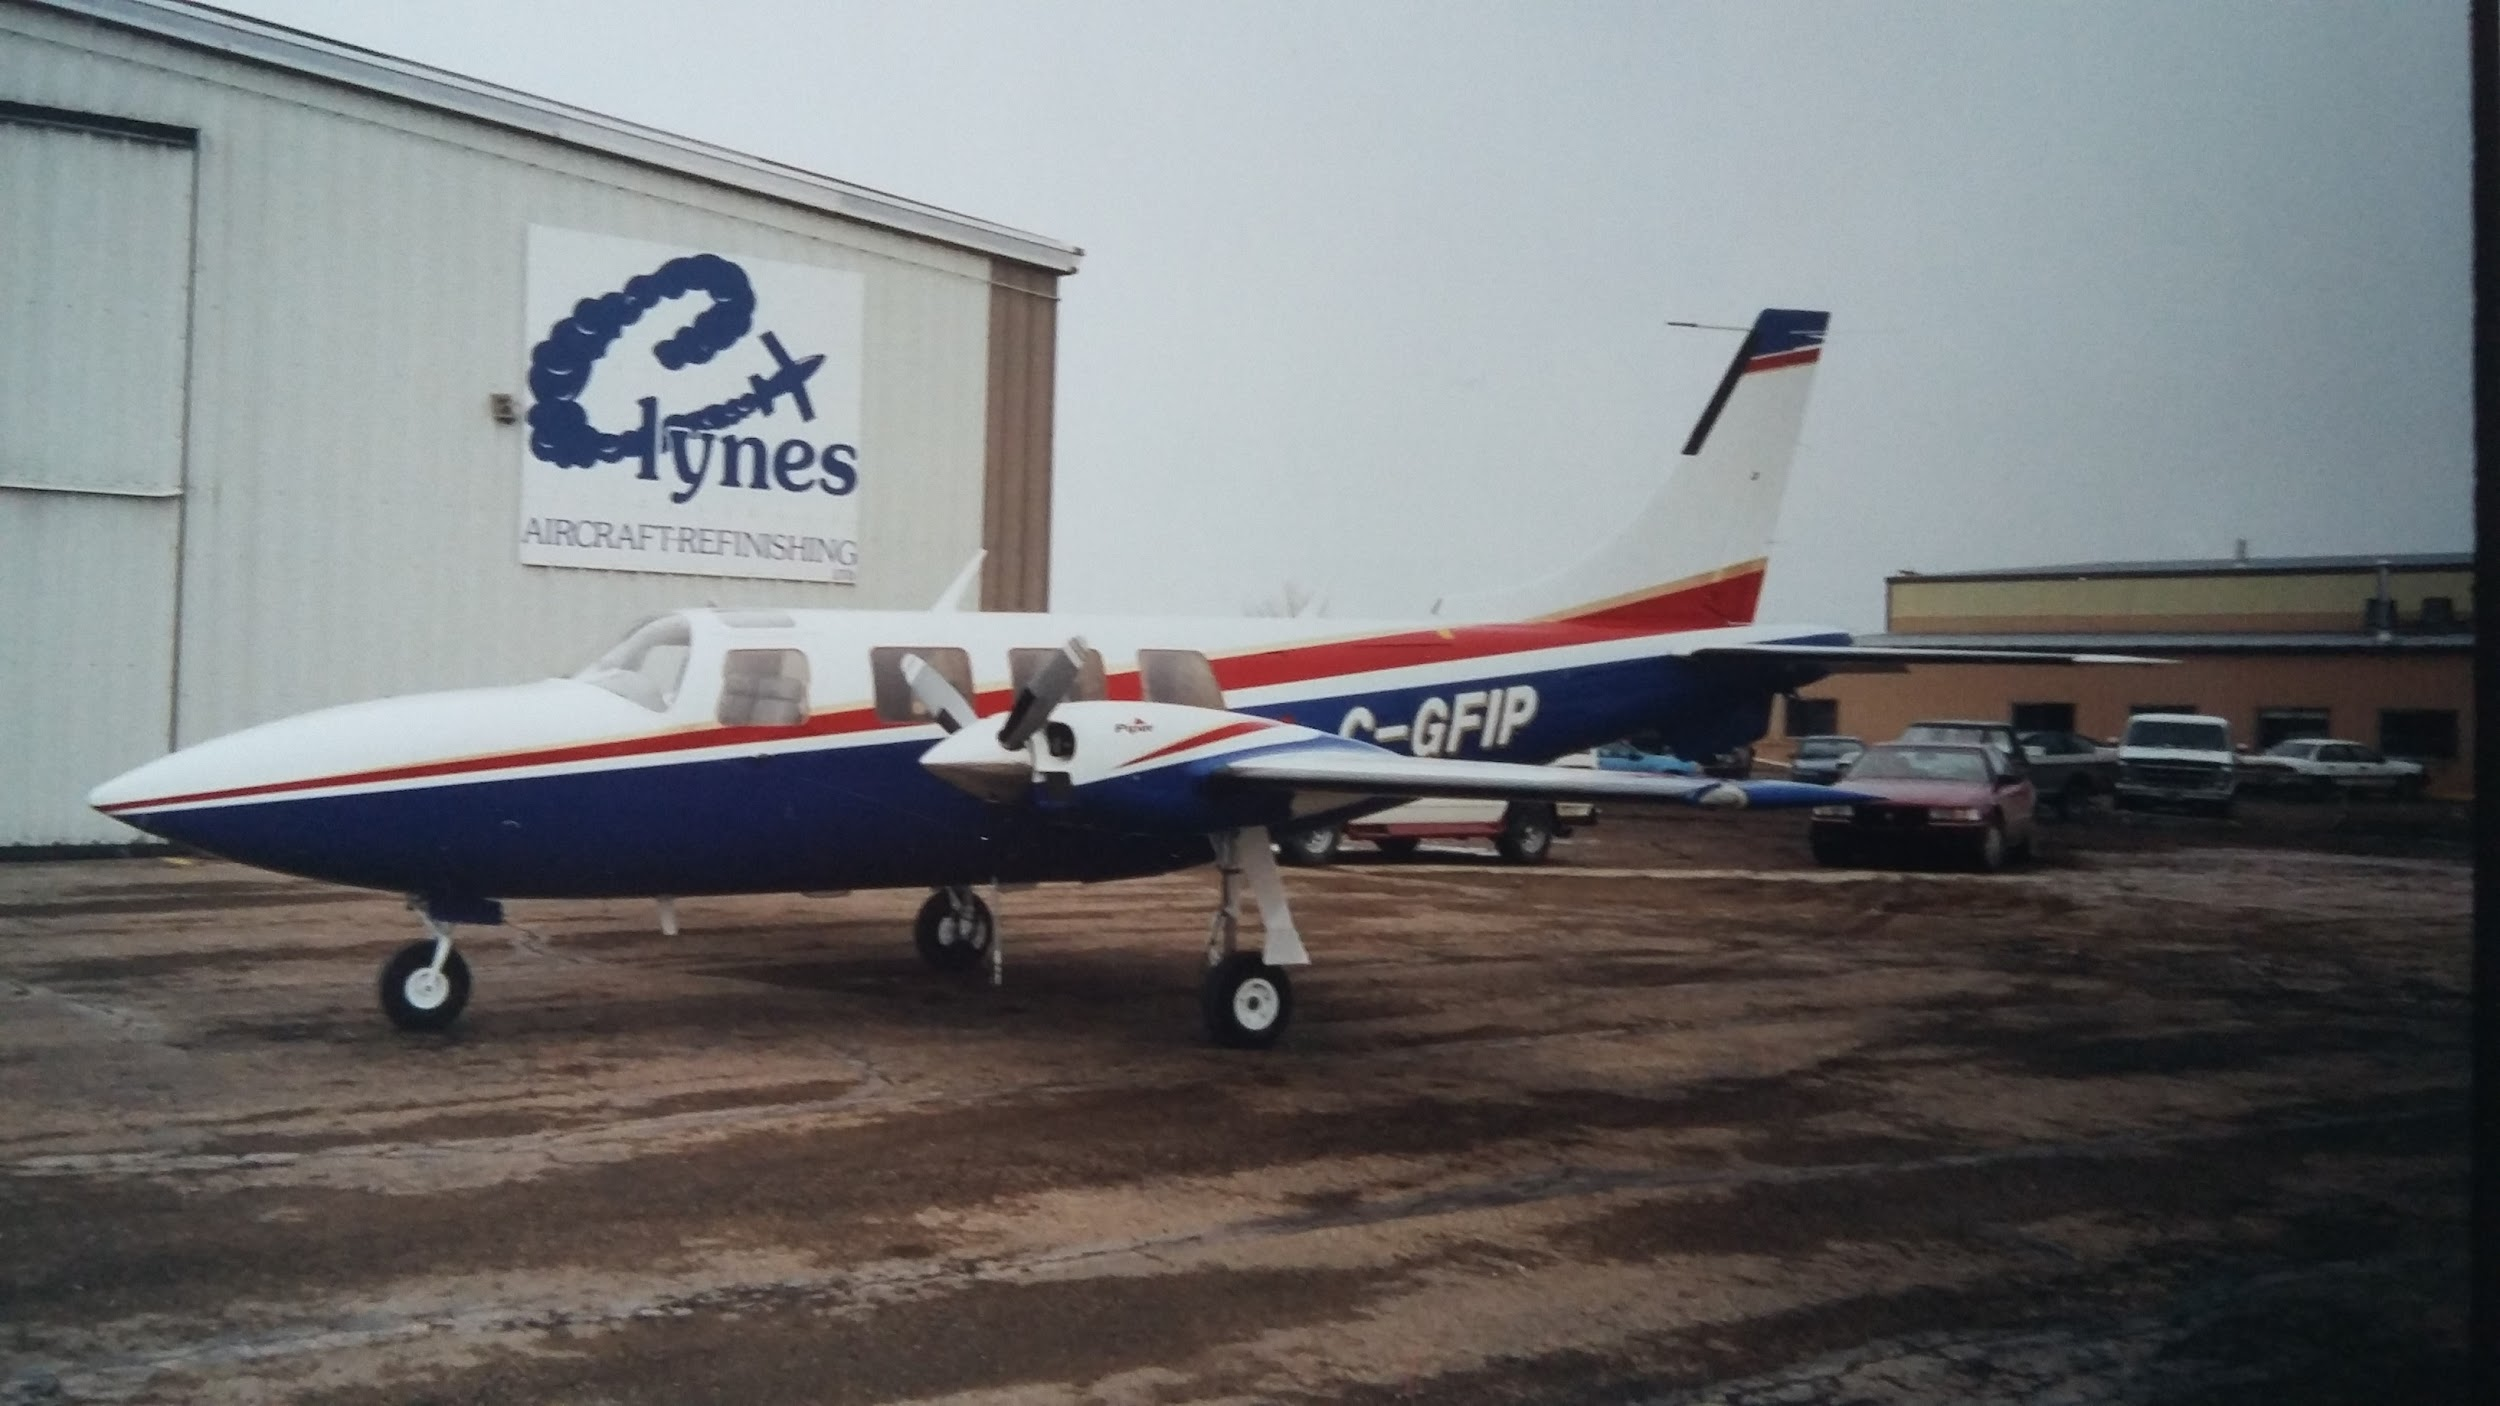
\includegraphics[scale=.2]{images/01.jpg}}
		\captionof{figure}{This is the final airplane of five that I owned. It is the Piper Aerostar pressurized twin engine aircraft that God supernaturally supplied (I gave the first one away to a missionary in Kenya and the four after that were miraculous provisions--you cannot outgive God). I made numerous mission trips into the high Arctic of Canada with it. This airplane was the one that I bought for \$99,000 and flew 200,000 miles; then I was able to sell it for \$240,000 to meet the bank’s demand.}
\end{minipage}\\
\clearpage

\chapter*{Some Testimonies from the Encounters Ministry}

\addtocontents{toc}{\protect\addvspace{10pt}}
\addtocontents{toc}{\textbf{APPENDIX}}

\end{document}